% ----------------------------------------
% Preambles
% ----------------------------------------
% ------- Set Document Class -------
\documentclass[11pt, draftcls]{ucdavisthesis}


% ------- Load Files Regarding Preambles -------
% 1. To load packages required
% ----------------------------------------
% Preamble: To load package(s) required
% ----------------------------------------
% ------- To load package(s) required -------
% 1. General
\usepackage[utf8]{inputenc}

% 2. To insert mathematical equations
\usepackage{amsmath, amssymb, amsthm, bbold, dsfont, mathabx}

% 3. To embed image files
\usepackage{graphicx}
\usepackage{caption, subcaption}
\usepackage{wrapfig}
\usepackage{afterpage}

% 4. To embed tables
\usepackage{longtable}
\usepackage{xtab, ltablex}
\usepackage{boldline, rotating, adjustbox}
\usepackage{makecell}
\usepackage{arydshln}

% 4.1. Tables from "fixest" library
\usepackage{booktabs}
\usepackage{threeparttable}
\usepackage{threeparttablex}
% % 4.2. Tables from "huxtable" library
% \usepackage{array}
% \usepackage{caption}
% \usepackage{graphicx}
% \usepackage{siunitx}
% \usepackage{ulem}
% \usepackage{colortbl}
% \usepackage{multirow}
% \usepackage{hhline}
% \usepackage{calc}
% \usepackage{tabularx}
% \usepackage{threeparttable}
% \usepackage{wrapfig}
% \usepackage{adjustbox}
% \usepackage{hyperref}

% 5. To generate figures
\usepackage{tikz}
\usetikzlibrary{intersections, through, calc, decorations.pathreplacing}

% 6. To change page mode
%\usepackage{lscape}
\usepackage{pdflscape}

% 7. To add a bibliography
\usepackage{natbib}

% 8. To add hyperlinks and set styles
\usepackage{hyperref}
\hypersetup{
    colorlinks = true,
    linkcolor = black,
    urlcolor = blue,
    citecolor = blue
}
\urlstyle{same}

% 9. To use multiple footnotes at one point
\usepackage[multiple]{footmisc}

% 10. Others
\usepackage{chngcntr}




% ----------------------------------------
% Doc. Setup & Info. for Preliminary Pages
% ----------------------------------------
% ------- Info. for Preliminary Pages -------
\title {
    Essays on Energy and Natural Resource Economics
}
% Exact title of your thesis. Indicate italics where necessary by underlining or using italics. Please capitalize the first letter of each word that would normally be capitalized in a title.

\author {
    \textsc{Jinmahn Jo}
}
% Your full name as it appears on University records. Do not use initials.

\authordegrees {
    \
}
% Indicate your previous degrees conferred.

\officialmajor {
    \textsc{Agricultural and Resource Economics}
}
% This is your official major as it appears on your University records.

\graduateprogram {
    Graduate Program Name
}
% This is your official graduate program name. Used for UMI abstract.

\degreeyear {
    2023
}
% Indicate the year in which your degree will be officially conferred.

\degreemonth {
    September
}
% Indicate the month in which your degree will be officially conferred. Used for UMI abstract.

\committee{Kevin Novan}{Katrina K. Jessoe}{Mark J. Agerton}{}{}
% These are your committee members. The command accepts up to five committee members so be sure to have five sets of braces, even if there are empties.


% ------- Copyright -------
%\copyrightyear{2020}
\nocopyright


% ------- Dedication -------
\dedication{
    \textsl{
        (To be added \ldots)
    }
}


% ------- Abstract -------
\abstract{
(To be added \ldots)
}


% ------- Acknowledgments -------
\acknowledgments{
(To be added \ldots)
}



% ----------------------------------------
% Main Document 
% ----------------------------------------
\begin{document}

\makeintropages
% Processes/produces the preliminary pages


% ------- Chapter 1 -------
\chapter{Dynamic Consumption Behavior with the Lagged Price Signals}
\label{Chapter:Chapter-1}

\section{Introduction}
\label{C1-Section:Introduction}
Increasing-Block Pricing (IBP) is one of the most common electricity rate plans.\footnote{As of the end of December 2022, about 40\% of the residential consumers of Pacific Gas and Electric Company (PG\&E), which is one of the largest utilities in California, were on the IBP.} Under the pricing scheme, the marginal price increases, in a nonlinear way, with the customer's usage. Specifically, the price consumers pay for their marginal electricity consumption is a step function of their aggregate consumption in a billing cycle. 

Economists have studied how residential consumers respond to nonlinear electricity pricing. \cite{Do-Consumers-Respond-to-Marginal-or-Average-Price?-Evidence-from-Nonlinear-Electricity-Pricing_2014_(Ito)} demonstrates that when faced with IBP, households respond to average prices rather than marginal prices. More recently, \cite{Misunderstanding-Nonlinear-Prices_2020_(Shaffer)} shows that not all households uniformly respond to the average price. To be specific, this paper exhibits that most residential consumers respond to the average price, but their response can be veiled by the response of a small number of households mistakenly applying the marginal price to all inframarginal units of consumption, not the last unit. And in both papers, it is stressed that households' misunderstanding of nonlinear electricity pricing leads to their inefficient electricity consumption, such as over- or under-consumption.

Electricity bills, usually issued every month, have been a primary, perhaps for some households the only, source of information about their electricity consumption (e.g., the total charges, the amount of consumption, and the marginal price). Inherently, the consumption-relevant information on a monthly electricity statement is not up to date---a statement principally includes information about the previous billing cycle. Household electricity consumption, however, is affected, at least partly, by the intermittent bills. As illustrated in \cite{Dynamic-Salience-with-Intermittent-Billing_Gilbert-and-Zivin_2014}, households change their consumption behavior after receiving a monthly bill. And in addition to the key finding discussed above, \cite{Do-Consumers-Respond-to-Marginal-or-Average-Price?-Evidence-from-Nonlinear-Electricity-Pricing_2014_(Ito)} presents convincing evidence that households respond more to lagged average prices, which are available in monthly electricity statements, than contemporaneous ones. 

There are two issues when residential consumers change their electricity consumption according to price signals delivered through monthly electricity bills. The first issue is that they respond to the incorrect prices. Whatever households' perceived price of nonlinear price schedules is, the price signals are false because these signals reflect not their contemporaneous consumption level but their past one. And households' exaggerated responses to the price signals are the second issue. Suppose that residential consumers adjust their electricity consumption according to the lagged prices. In that case, the behavioral change implies that all consumption in a billing cycle is subject to the previous billing cycle's prices. Importantly, such an implication is analogous with households' over-responses to the (current) marginal price discussed in \cite{Misunderstanding-Nonlinear-Prices_2020_(Shaffer)}. 

On both those fronts, this paper examines households' responses to the marginal price again. For residential consumers under IBP, I measure how much electricity consumption they reduce in a billing month following the marginal price's discontinuous increase at a base usage quantity in the previous billing month, which is not accompanied by any changes in the average price. In other words, focusing on two consecutive billing cycles, I investigate how households respond to the sharp increase in the \textit{lagged} marginal price signaled through their monthly electricity bills.

To estimate the impact of the change in the marginal price due to surpassing a base usage quantity in a billing cycle on household electricity consumption in the following billing cycle, I adopt a Regression Discontinuity (RD) approach that exploits the sharp discontinuity in the marginal price at the threshold. Under IBP, a household's (within-billing-cycle) aggregate electricity consumption at some point completely determines the price the household pays for the marginal unit of consumption at that point. Considering the known-to-consumer price determination mechanism, it appears that households can flexibly alter their electricity demand not to consume more than a base usage quantity, at which the marginal price discontinuously increases. In my empirical setting, however, it is not convincing for two reasons. First of all, the households in my sample had no practical way to know how much electricity they had consumed from the first day of a billing cycle to the point of marginal electricity consumption, especially before installing smart meters. They were able to find out whether their total consumption in a billing cycle surpassed the threshold only after receiving their monthly bills at the beginning of the subsequent billing cycle. On top of that, it is not feasible for them to adjust their electricity consumption precisely to avoid crossing the cutoff point due to their indispensable consumption (e.g., consumption for refrigerators and lighting) and too high information cost imposed when micromanaging electricity demand according to the change of outdoor conditions. Thus, the two points demonstrate that my RD design clearly satisfies the fundamental assumption required for identification: around the threshold, the treatment assignment is random.

Implementing the RD design to monthly billing records from hundreds of thousands of residential consumers in Sacramento, CA, I find households' interesting behavioral change with respect to electricity consumption: around the lower base usage quantity, the households that were subject to a higher marginal price because their aggregate electricity consumption in a billing month exceeded the cutoff point reduced their average daily electricity consumption by 0.1\% in the following billing month, compared to the households experiencing no change in the marginal price. Because only the marginal price discontinuously increased, not the average price, at the threshold, this result is convincing evidence that households, conservatively at least some of them, respond to marginal prices. In line with \cite{Misunderstanding-Nonlinear-Prices_2020_(Shaffer)}, if the identified reduction in household electricity consumption is entirely attributable to behavioral changes of a subset of residential consumers, my estimates imply that less than 5\% of households in my sample reacted to the discontinuous jump in the marginal price. More importantly, the result suggests another inefficiency stemming from households' responses to nonlinear electricity pricing: 1) households also respond to the lagged marginal price, which is irrelevant to their present consumption level; and 2) the lagged marginal price is applied to all units of electricity consumption, not the last unit, during a billing cycle. 

I also examine heterogeneity in households' responsiveness to the lagged marginal price across rate codes and seasons. Furthermore, my investigation into the impacts of the discontinuous increase in the marginal price on household electricity consumption demonstrates that reductions in household electricity consumption persist over multiple billing cycles but tend to dissipate gradually. 

The rest of this paper proceeds as follows. In Section 2, I discuss my empirical approach and data. Section 3 presents the results from my empirical analysis. Section 4 describes the policy implications of my key findings, and Section 5 concludes. 



\section{Data and Research Design}
\label{C1-Section:Data-and-Research-Design}
This section provides a detailed description of the data utilized for my empirical analysis. Furthermore, this section demonstrates a key feature of my research design.


% Institutional Background
\subsection{Background of Residential Rates of Sacramento Municipal Utility District}
\label{C1-Sub-section:Background-of-Residential-Rates-of-SMUD}
Sacramento Municipal Utility District (SMUD), which is the nation's sixth-largest community-owned electric utility, provides electricity to most of Sacramento County and small portions of adjoining Placer and Yolo Counties.\footnote{According to the company information presented on \href{https://www.smud.org/en/Corporate/About-us/Company-Information}{SMUD's website}, the size of this utility's service area is about 900 square miles.}

\afterpage{
    \begin{figure}[t!]
        \centering
        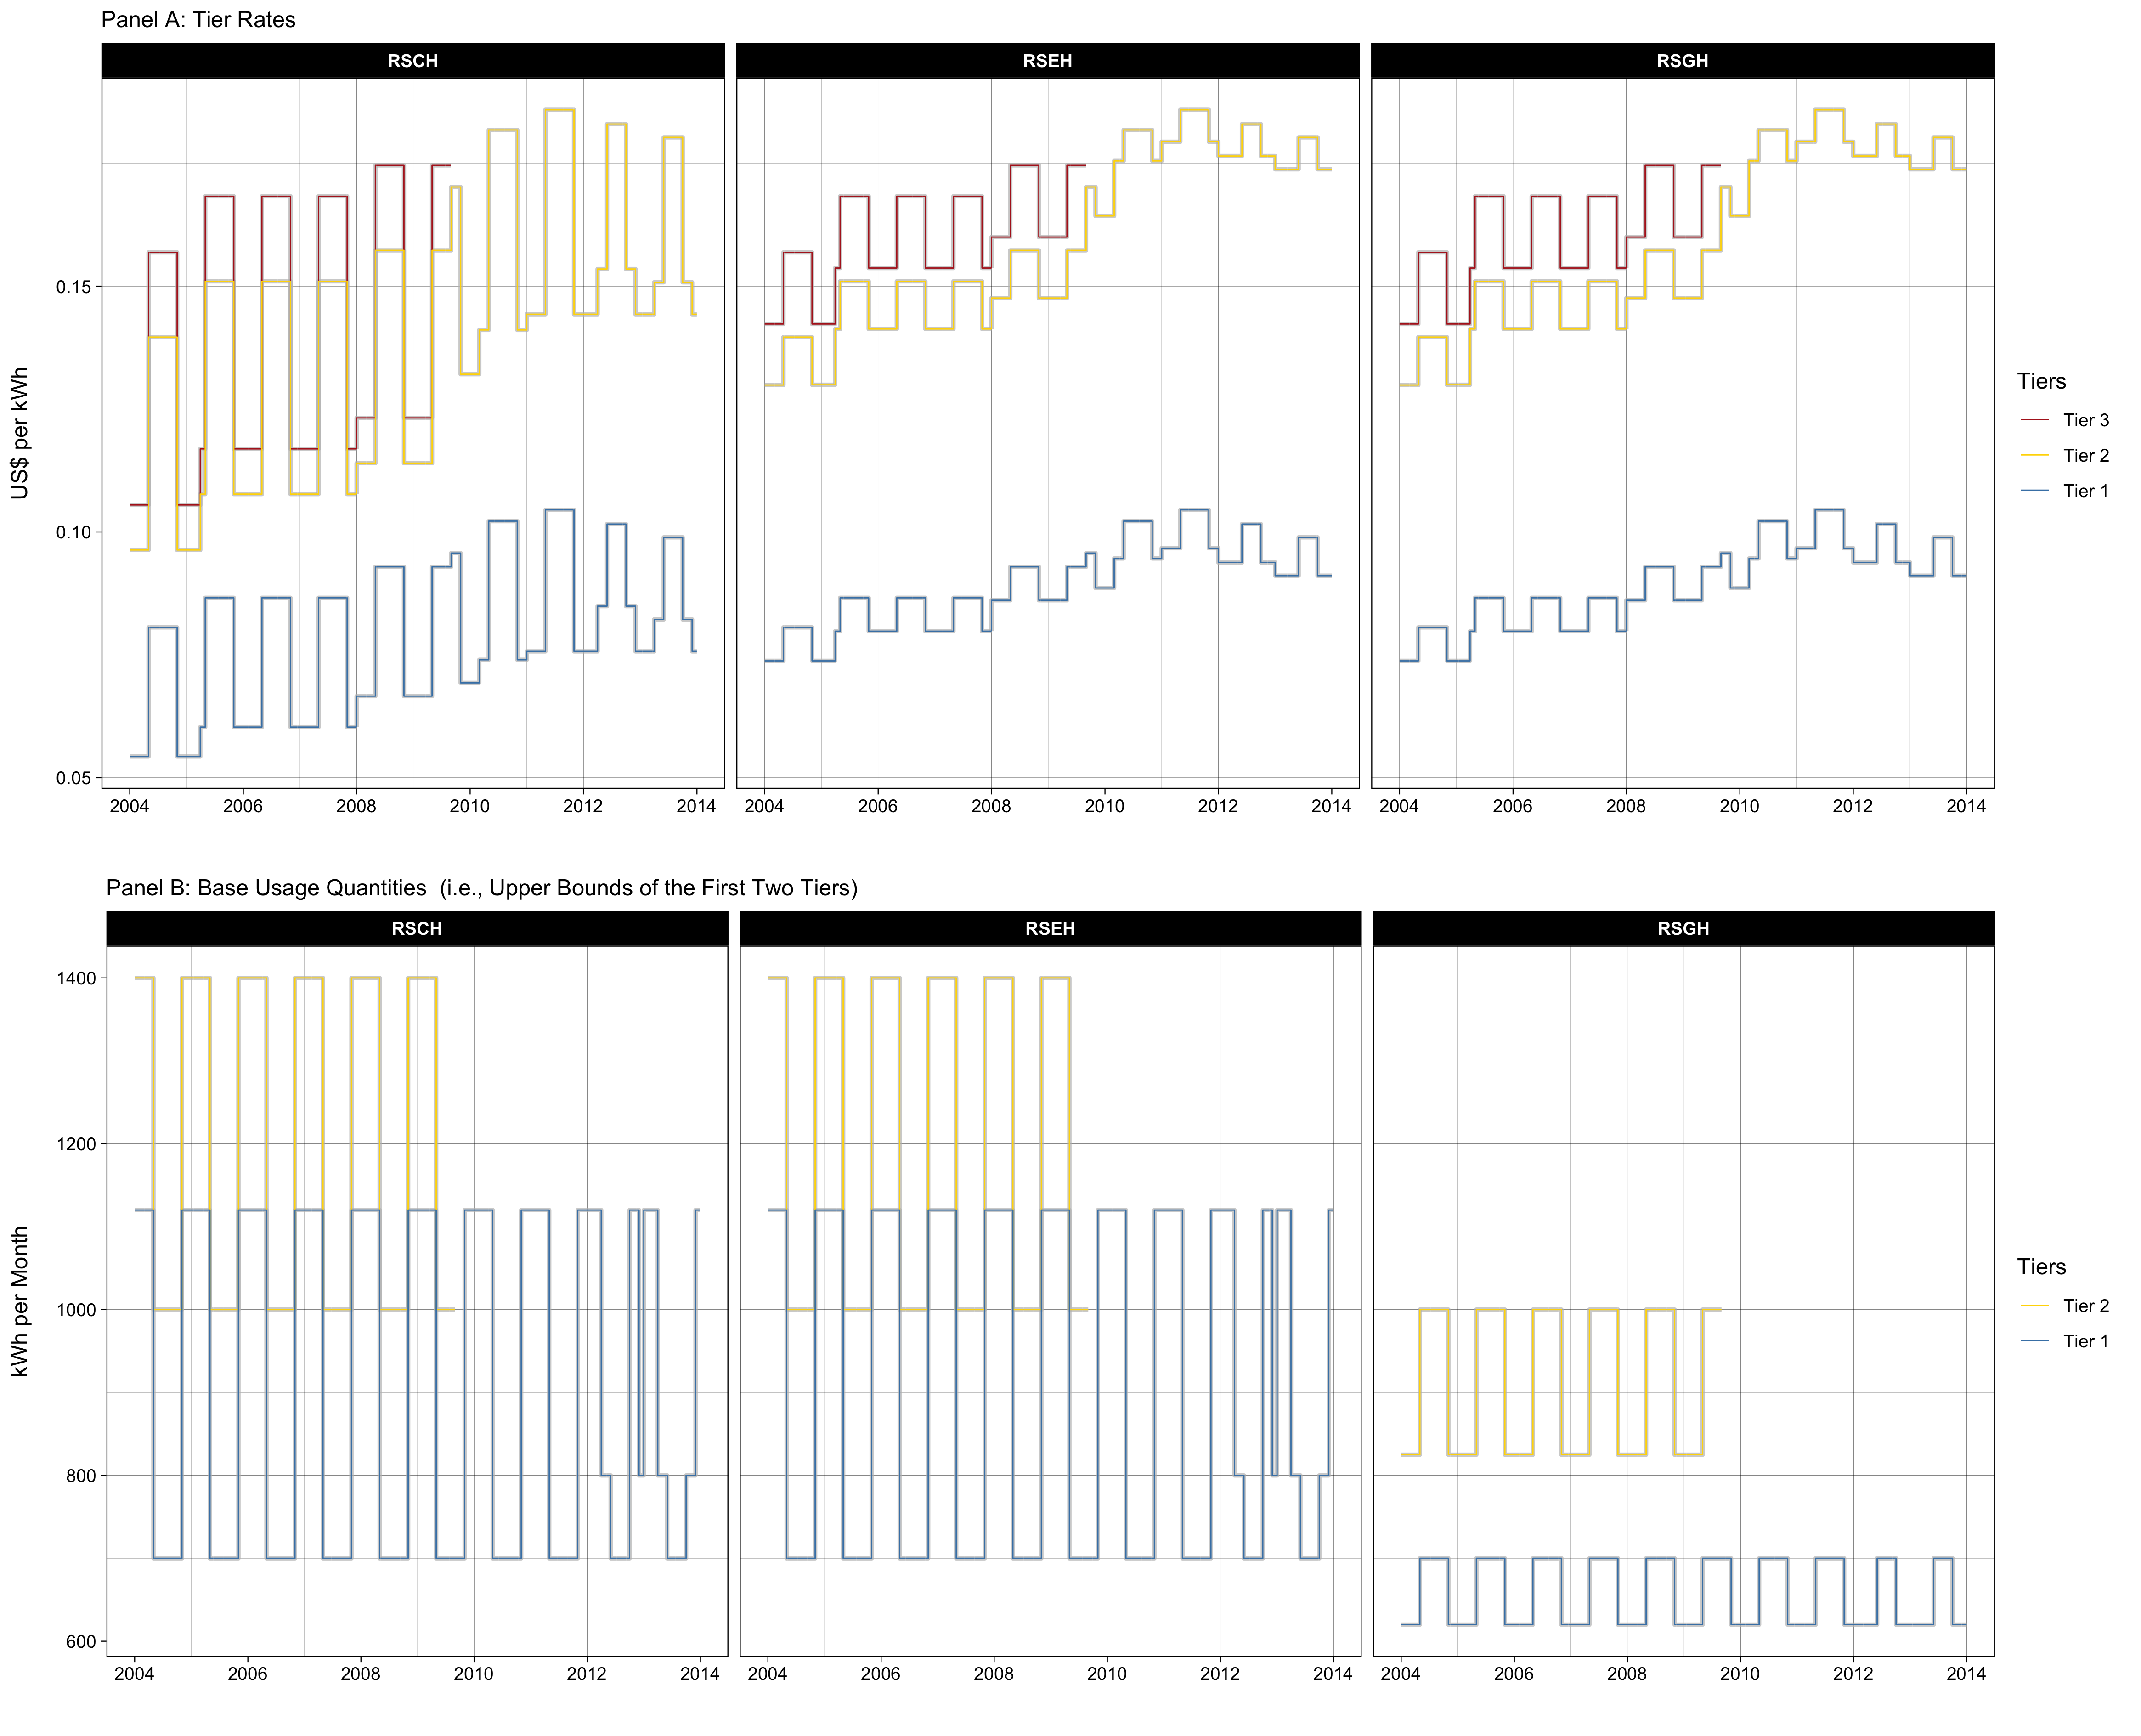
\includegraphics[scale = 0.097]{02_Chapter-1/00A_Figures/Figure_SMUD-Residential-Rates_Variable-Charges-and-Base-Usage-Quantities.png}
        \caption{Tier Rates and Base Usage Quantities of SMUD Residential Rates}
        \caption*{
            {\small
            \textit{Note}: 
            The figure illustrates how SMUD changed tier rates and base usage quantities of the three major residential rate plans (i.e., RSCH, RSEH, and RSGH) over time. Both tier rates and base usage quantities show significant seasonality. The two rate plans for electric-heating households (i.e., RSCH and RSEH) had the same base usage quantities. There have been only two tiers since September 2009.
        }}
        \label{Figure:SMUD-Residential-Rates_Variable-Charge-and-Base-Usage}
    \end{figure}
}
Before the default residential rate switched to the Time-Of-Day (TOD) rate, most SMUD residential customers chose residential rates having an increasing nonlinear block-tier structure.\footnote{In my sample, only 5\% of residential customers adopted the TOD rate, although SMUD already offered it.} The three most popular rates for SMUD residential customers were Standard General Service (RSGH), Standard Closed Electric-Heated Service (RSCH), and Standard Open Electric-Heated Service (RSEH).\footnote{Specifically, more than 75\% of SMUD residential customers in my dataset chose the RSGH rate, whereas 2\% and 20\% of households in my dataset adopted the RSCH and RSEH rates, respectively.} For those residential rates, the marginal price of the energy charge was a step function of monthly consumption relative to a base usage quantity per month, which varies seasonally. Figure \ref{Figure:SMUD-Residential-Rates_Variable-Charge-and-Base-Usage} illustrates variations in price and base usage quantity over time. Two points are noteworthy from this figure: first, both tier rates and base usage quantities of the energy charges showed substantial seasonality; second, the structure of the residential rates changed from three-tier to two-tier since September 2009.

In addition to the variable charge (i.e., the energy charge), households choosing one of the three rates should pay a per-month fixed charge, called the System Infrastructure Fixed Charge. As shown in Figure \ref{Figure:SMUD-Residential-Rates_Fixed-Charge}, the unit price of the fixed charge significantly increased between 2009 and 2014. 




% Data and Summary Statistics
\subsection{Data and Summary Statistics}
\label{C1-Sub-section:Data-and-Summary-Statistics}
From SMUD, I obtain household-level monthly billing history of residential consumers in the Sacramento area from 2004 to 2013. For each monthly record, account ID, premise ID, rate code, billing start and end dates, monthly consumption with its breakdown into each tier, monthly fixed charge, monthly variable charge only for kWh usage, total monthly bill, and an indicator related to solar adoption are included in the data. Of note, in my empirical analysis, I assume that a pair of account and premise IDs corresponds to an individual household. And because the monthly billing data contain no price and base usage quantity information, I append historical price schedules and base usage quantities presented by SMUD. Unfortunately, my monthly billing data also lack any socioeconomic and demographic information. 

First, I focus on households that consistently used one of the three major residential rates (i.e., RSGH, RSCH, and RSEH) in their billing history. Second, I only utilize billing records before 2010, from which SMUD got down to install smart meters. Third, I focus on households whose number of billing periods is greater than or equal to 24. Fourth, I focus on SMUD residential customers with reliable billing records only.\footnote{To be specific, I exclude, from the sample used for my empirical analysis, households that have billing records being applied to any of the following conditions: 1) observations whose length of the billing period is either less than 27 or greater than 34; 2) observations with negative values for either quantities or charges; 3) observations having overlapping billing periods within a pair of account and premise IDs; and 4) observations whose number of days from the previous billing period is greater than 14.} Fifth, my sample only includes households that crossed the lower threshold at least once in their billing history.\footnote{In other words, I drop always-light- and always-heavy-users from my sample. } The procedure results in 16,322,353 billing records for 365,975 households. Table \ref{Table:Summary-Statistics} provides summary statistics for my sample. Furthermore, Figure \ref{Figure:Household-Average-Daily-Electricity-Consumption-by-Month-of-Year} shows, for each rate code, households' average daily electricity consumption by month of the year. 

To take account of the impact of weather conditions, especially outdoor temperatures, on household electricity consumption, I utilize the Local Climatological Data (LCD) for the Sacramento International Airport, published by the National Oceanic and Atmospheric Administration (NOAA). Using daily heating degree days (HDDs) and daily cooling degree days (CDDs) in the LCD between 2004 and 2009, I calculate each monthly billing period's accumulated HDDs and CDDs, which are used to compute the average daily HDDs and CDDs. 




% Research Design
\subsection{Research Design}
\label{C1-Sub-Section:Research-Design}

\subsubsection{Monthly Bill as the Only Source of Electric Usage Information for Households}
\label{C1-Sub-Sub-section:Monthly-Bill-as-the-Only-Source-of-Electric-Usage-Information-for-Households}
Before 2009, there was no feasible way for SMUD residential customers to access real-time information related to their electricity use. SMUD initiated installations of smart meters, allowing its residential and business customers to view their electricity usage online when they want, in late 2009. The electric service completed it in the first quarter of 2012. Also, the three types of bill alert SMUD are offering were introduced in 2017.\footnote{SMUD provides its customers with three types of bill alerts, via text or e-mail, as a billing service: 1) Mid-Bill Alerts send an alert on the 16th day of a customer's billing period and advise what his usage has been and what the cost is as of that day, 2) High Bill Alters compare a customer's current billing cycle to the same billing cycle in the previous year and alerts the customer if their current usage is running higher than before, and 3) Bill Threshold allows a customer to know when his bill has reached a certain amount set in advance by himself.} Therefore, for households using SMUD-delivering electricity, the only practical source of information about their electricity consumption had been their monthly bill statements, which send out (either e-mail or U.S. mail) after 3 or 4 business days from the last day of each billing cycle. 

The issue of households' welfare losses due to their response to discontinuous changes in the lagged marginal price suggests the importance of providing seemly price information in an appropriate manner. Many studies about various time-varying electricity pricing show that households changed their consumption behavior in response to the information about consumption and prices \citep{Dynamic-Pricing-of-Electricity-in-the-Mid-Atlantic-Region_Econometric-Results-from-the-Baltimore-Gas-and-Electric-Company-Experiment_Faruqui-et-al_2011, Knowledge-is-Less-Power_Jessoe-and-Rapson_2014, The-Effect-of-Information-on-TOU-Electricity-Use:An-Irish-Residential-Study_Pon_2017, Information-vs-Automation-and-Implications-for-Dynamic-Pricing_Bollinger-and-Hartmann_2020}. My empirical finding demonstrates that even under IBP, such information, though lagged, still plays a role in household electricity consumption. In this respect, providing household-specific as well as current price information for residential consumers, via text messages or app notifications regularly, could encourage them to respond to \textit{true} price signals rather than lagged ones, which in turn avoid the negative impact on household welfare. Based on the dissipating effect of intermittently salient information discussed in \cite{Dynamic-Salience-with-Intermittent-Billing_Gilbert-and-Zivin_2014}, a high frequency of informing the latest tailored price information might maximize households' behavior change in electricity consumption. In addition, because sending such information-bearing notifications is available at a very low cost these days, this type of information provision would be a practical policy instrument for utilities, especially in developing countries where the transition toward dynamic electricity pricing is difficult due to substantial investments in installing smart metering systems. 


\subsubsection{Regression Discontinuity Design}
\label{C1-Sub-Sub-Section:Regression-Discontinuity-Design}
In this paper, I employ a Regression Discontinuity (RD) design to examine how households' electricity consumption responds to the marginal price informed via monthly energy statements under Increasing-Block Pricing (IBP). In previous studies, a common challenge in measuring consumption responses to price changes has been discussed repeatedly: constructing a well-defined control group is difficult due to that consumers typically experience the same price variation. However, the setting I exploit in this paper enables me to address the identification challenge.  

The RD design I implement in this paper relies on three points. First, the marginal price is a step function of consumption level in the increasing block-tier rate plans chosen by SMUD residential customers. That is, under IBP, the price a household pays for the marginal electricity consumption increases discontinuously at some pre-determined aggregate consumption in a billing cycle. Second, as discussed in Section \ref{C1-Sub-Sub-section:Monthly-Bill-as-the-Only-Source-of-Electric-Usage-Information-for-Households}, before 2009, SMUD residential customers had practically no way to know the marginal price in a billing cycle within the very cycle. They were informed of the price they paid for the marginal electricity consumption in a billing cycle only through their electricity bills delivered in the following cycle. Third, it is not generally feasible for households to consume only a pre-targeted amount of electricity within a billing cycle. In general, households have limited capability to control their electricity consumption due to the minimal essential demand (e.g., usage for refrigerators and lighting). In addition, because household electricity consumption heavily depends on outdoor temperature variation, managing one's own electricity usage not to exceed the target amount of electricity consumption could incur too high information cost, which might result in rational inattention \citep{Rational-Inattention-and-Energy-Efficiency_Sallee_(2014)}, even if households are available to adjust their consumption behavior with complete flexibility. 

\afterpage{
    \begin{figure}[t!]
        \centering
        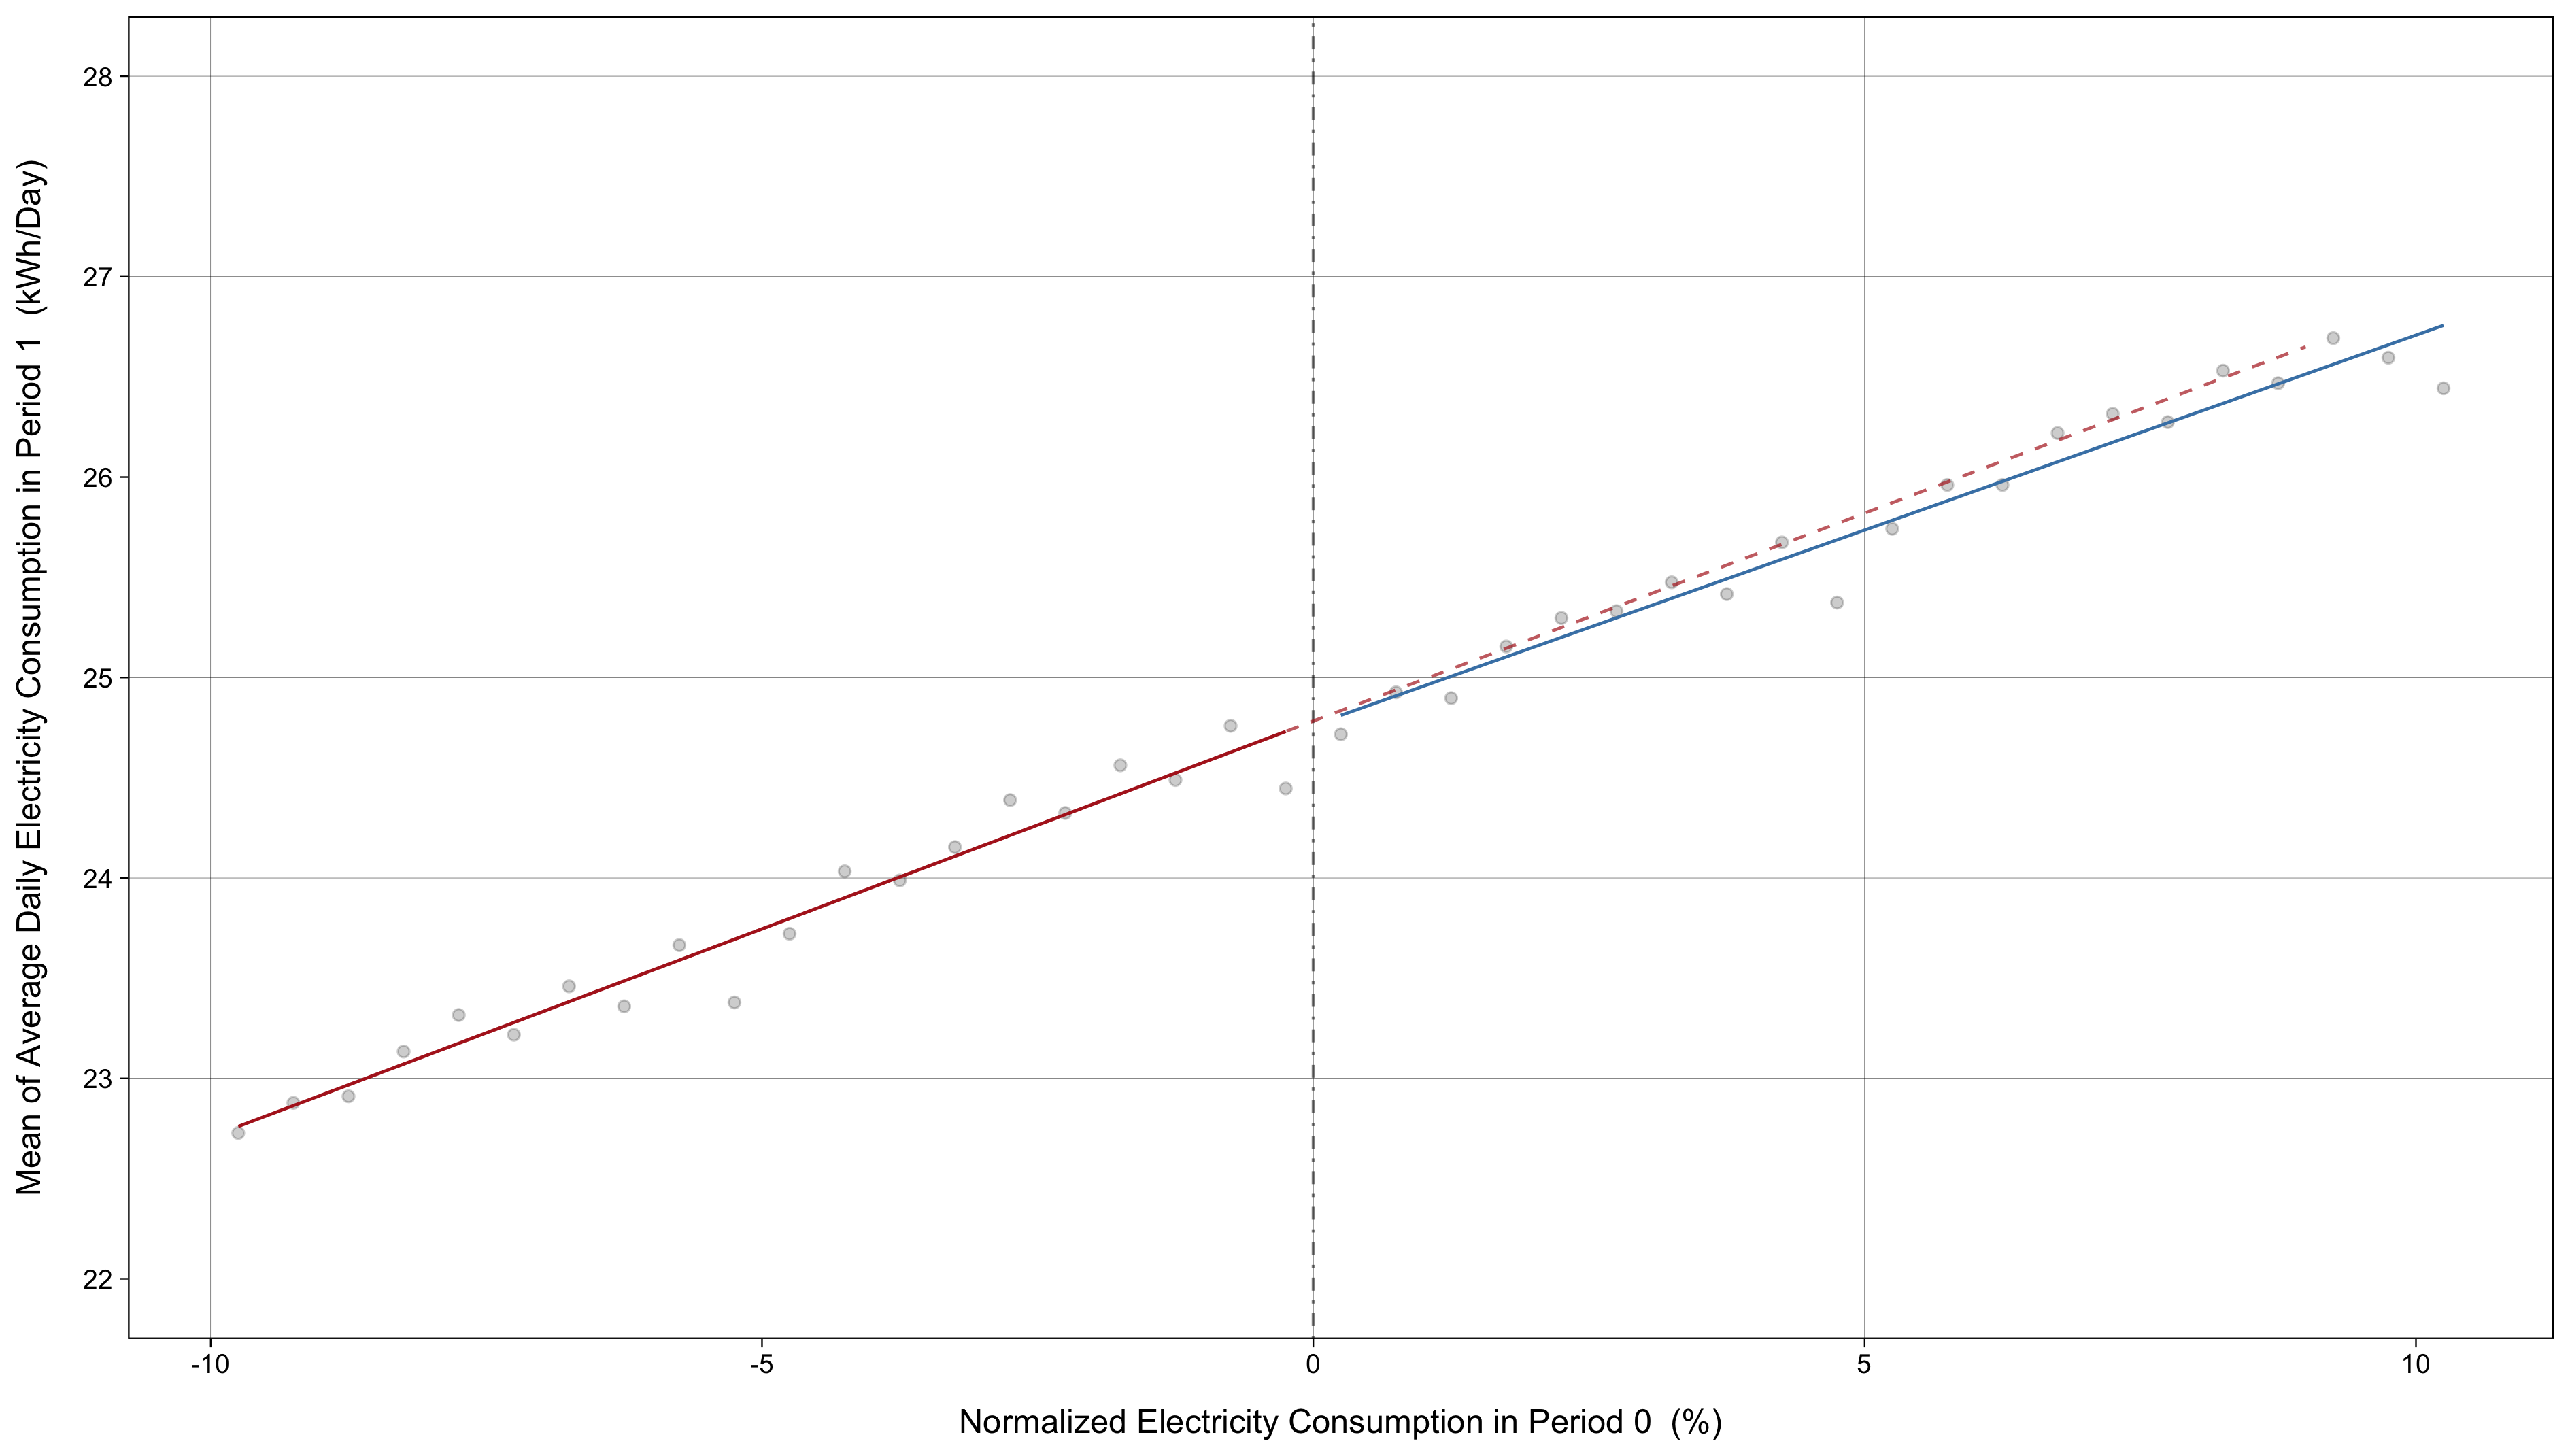
\includegraphics[scale = 0.115]{02_Chapter-1/00A_Figures/Figure_Average-Daily-Electricity-Consumption-in-Period-1-over-NC0.png}
        \caption{Mean of Average Daily Electricity Consumption in Period 1 over $\overline{NC}_{0}$}
        \caption*{
            {\small
            \textit{Note}: 
            This figure's scatter points correspond to the average daily electricity consumption in Period 1, computed by bins with a bandwidth of 1\% of $\overline{NC}_{0}$. The solid line on each side of the vertical dot-dash line is a parametric fit obtained from the regression of the average daily electricity consumption on $\overline{NC}_{0}$. The dashed red line is an extension of the solid red line. The gap between the dashed red and solid blue lines seems to indicate a non-negligible treatment effect. 
        }}
        \label{Figure:Average-Daily-Electricity-Consumption-in-Period-1-over-NC0}
    \end{figure}
}
Regarding the first point, the discontinuities under the nonlinear electricity schedules allow utilizing a RD design. In my RD design, the running variable is the level of electricity consumption in a household during a billing period (denoted as Period 0), whereas the outcome variable corresponds to the household's average daily electricity consumption during the subsequent billing period (denoted as Period 1). So, in this quasi-experimental setting, I compare SMUD residential customers just above and below the thresholds of the tier rates, called base usage quantities. Under IBP, surpassing a threshold leads to an increase in the marginal price households pay for electricity consumption mechanically. Here, the discontinuous increase in the marginal price, which accompanies \textit{no discontinuous change in the average price}, applies only to Period 0, not to Period 1.\footnote{The average price smoothly grows around the cutoff point.} Moreover, information about whether households were subject to a higher marginal price in a billing period is delivered early in the subsequent billing period through their monthly electricity bills. Therefore, any changes with respect to the electricity consumption of households just above the threshold (i.e., households in the treatment group) in Period 1, compared to households just below the threshold (i.e., households in the control group), can be understood as their short-term behavioral responses stemming from the sharp jump in the marginal price in Period 0. Figure \ref{Figure:Average-Daily-Electricity-Consumption-in-Period-1-over-NC0}, showing how the mean of households' average daily electricity consumption in Period 1 evolves around the lower base usage quantity, seems to indicate the existence of such behavioral responses. 

The last two points demonstrate that the fundamental identifying assumption of the RD design is reasonable. The fundamental identifying assumption is that SMUD residential customers just below a base usage quantity are expected to be very similar to those just above it, along with observed and unobserved characteristics. In other words, a group of households in the small neighborhood of the threshold is not different from one obtained from a randomized experiment. In my setting for empirical analysis, SMUD residential customers were unable to be aware of how far away they were from a given cutoff point in real time. Furthermore, as discussed above, it is not convincing that they can perfectly control their electricity consumption during a billing cycle to use exactly a target amount of electricity by the end of the last day of the billing cycle. Hence, it is highly unlikely that the customers precisely adjusted their consumption behavior so as to avoid surpassing the cutoff point, which in turn prevented them from leading to a higher marginal price. That is, it seems plausible that households were not able to sort themselves around the threshold strategically. Therefore, any discontinuity gap in the outcome variable can be attributed to the discontinuous increase in the marginal price at the threshold in Period 0. 


\subsubsection{The Validity of the Regression Discontinuity Design}
\label{C1-Sub-Sub-Section:The-Validity-of-the-Regression-Discontinuity-Design}
\afterpage{
    \begin{figure}[t!]
        \centering
        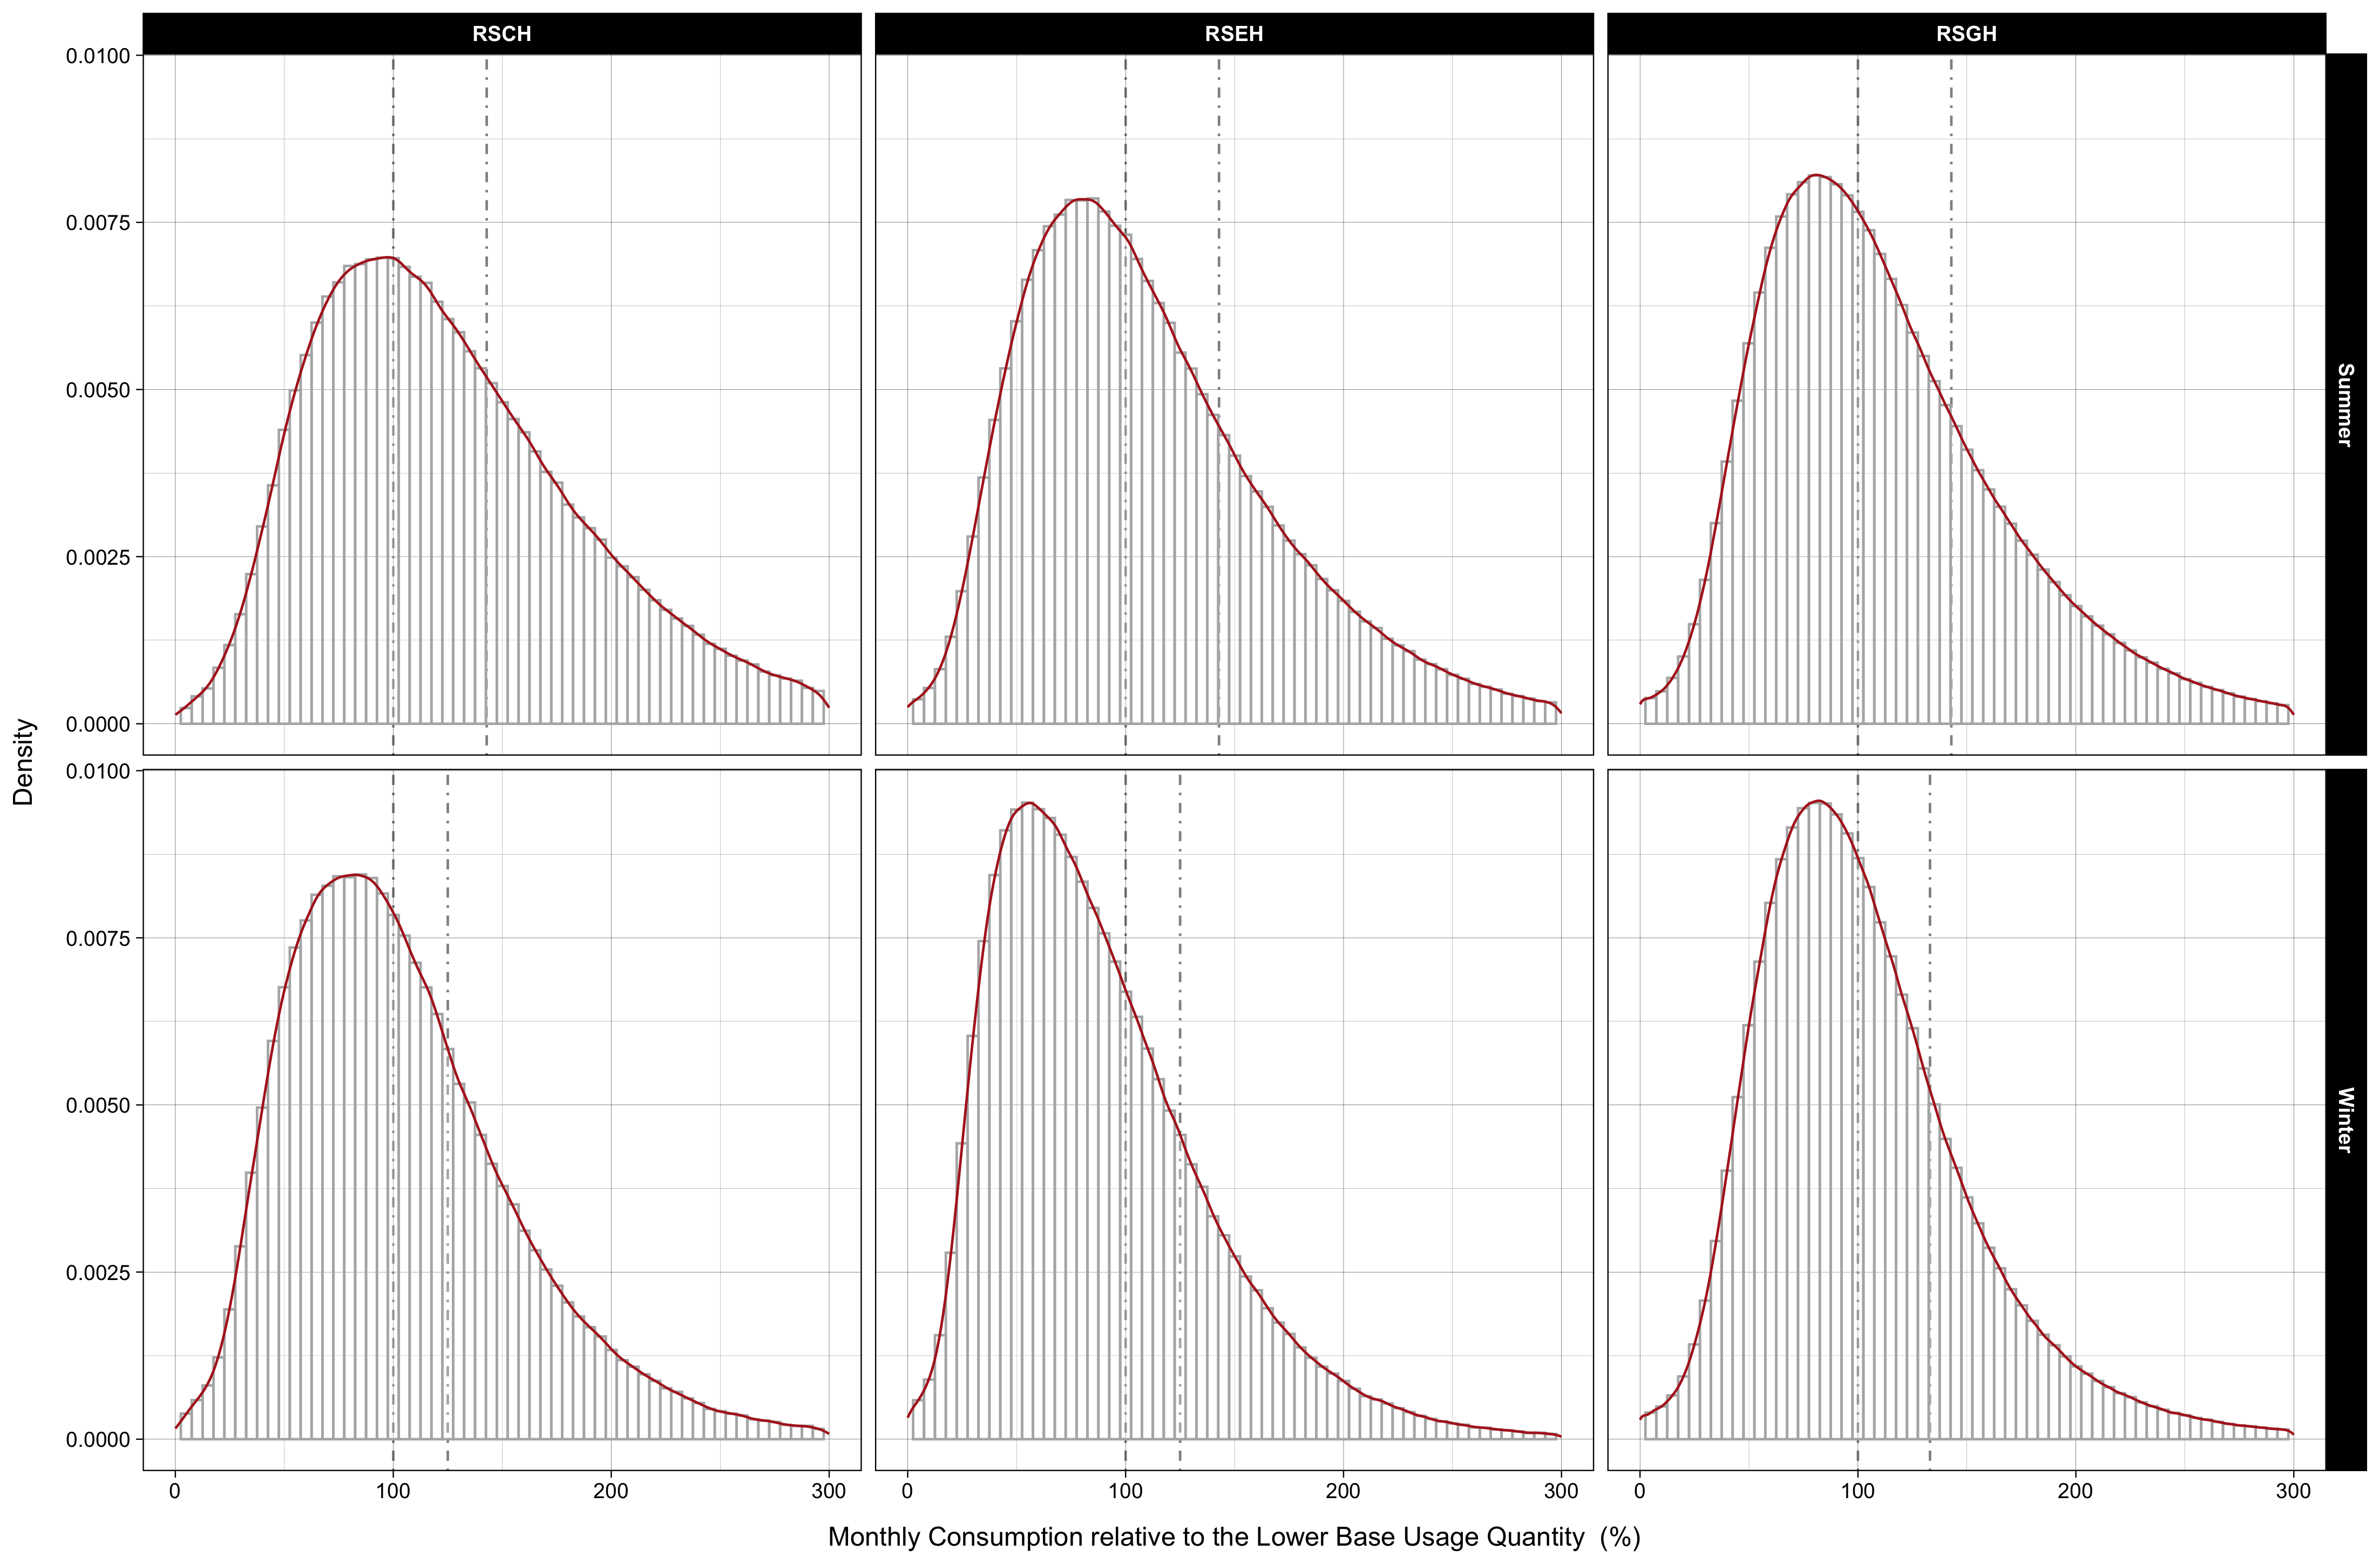
\includegraphics[scale = 0.101]{02_Chapter-1/00A_Figures/Figure_Distribution-of-Electricity-Consumption.png}
        \caption{Distribution of Electricity Consumption by SMUD Residential Customers}
        \caption*{
            {\small
            \textit{Note}: 
            This figure presents histograms, with kernel density estimates, for electricity consumption by SMUD residential customers. Each of the six panels in the figure is for a pair of three major residential rates (i.e., RSCH, RSEH, and RSGH) and two seasons (i.e., summer and winter). Dot-dashed vertical lines in each panel are base usage quantities for the corresponding rate code and season.
        }}
        \label{Figure:SMUD-Billing-Data_Histogram_By-Season-and-Rate-Code}
    \end{figure}
}
Two pieces of evidence support the assumption that base usage quantities do not correspond to jumps in household characteristics. First, as illustrated in Figure \ref{Figure:SMUD-Billing-Data_Histogram_By-Season-and-Rate-Code}, each density plot of the running variable is very smooth, without any bump (i.e., excess mass), around base usage quantities at which marginal prices jump. The set of density plots that show apparent continuity at the thresholds suggests households' inability to precisely adjust their electricity consumption in order not to be subject to a higher marginal price. 

\afterpage{
    \begin{figure}[t!]
        \centering
        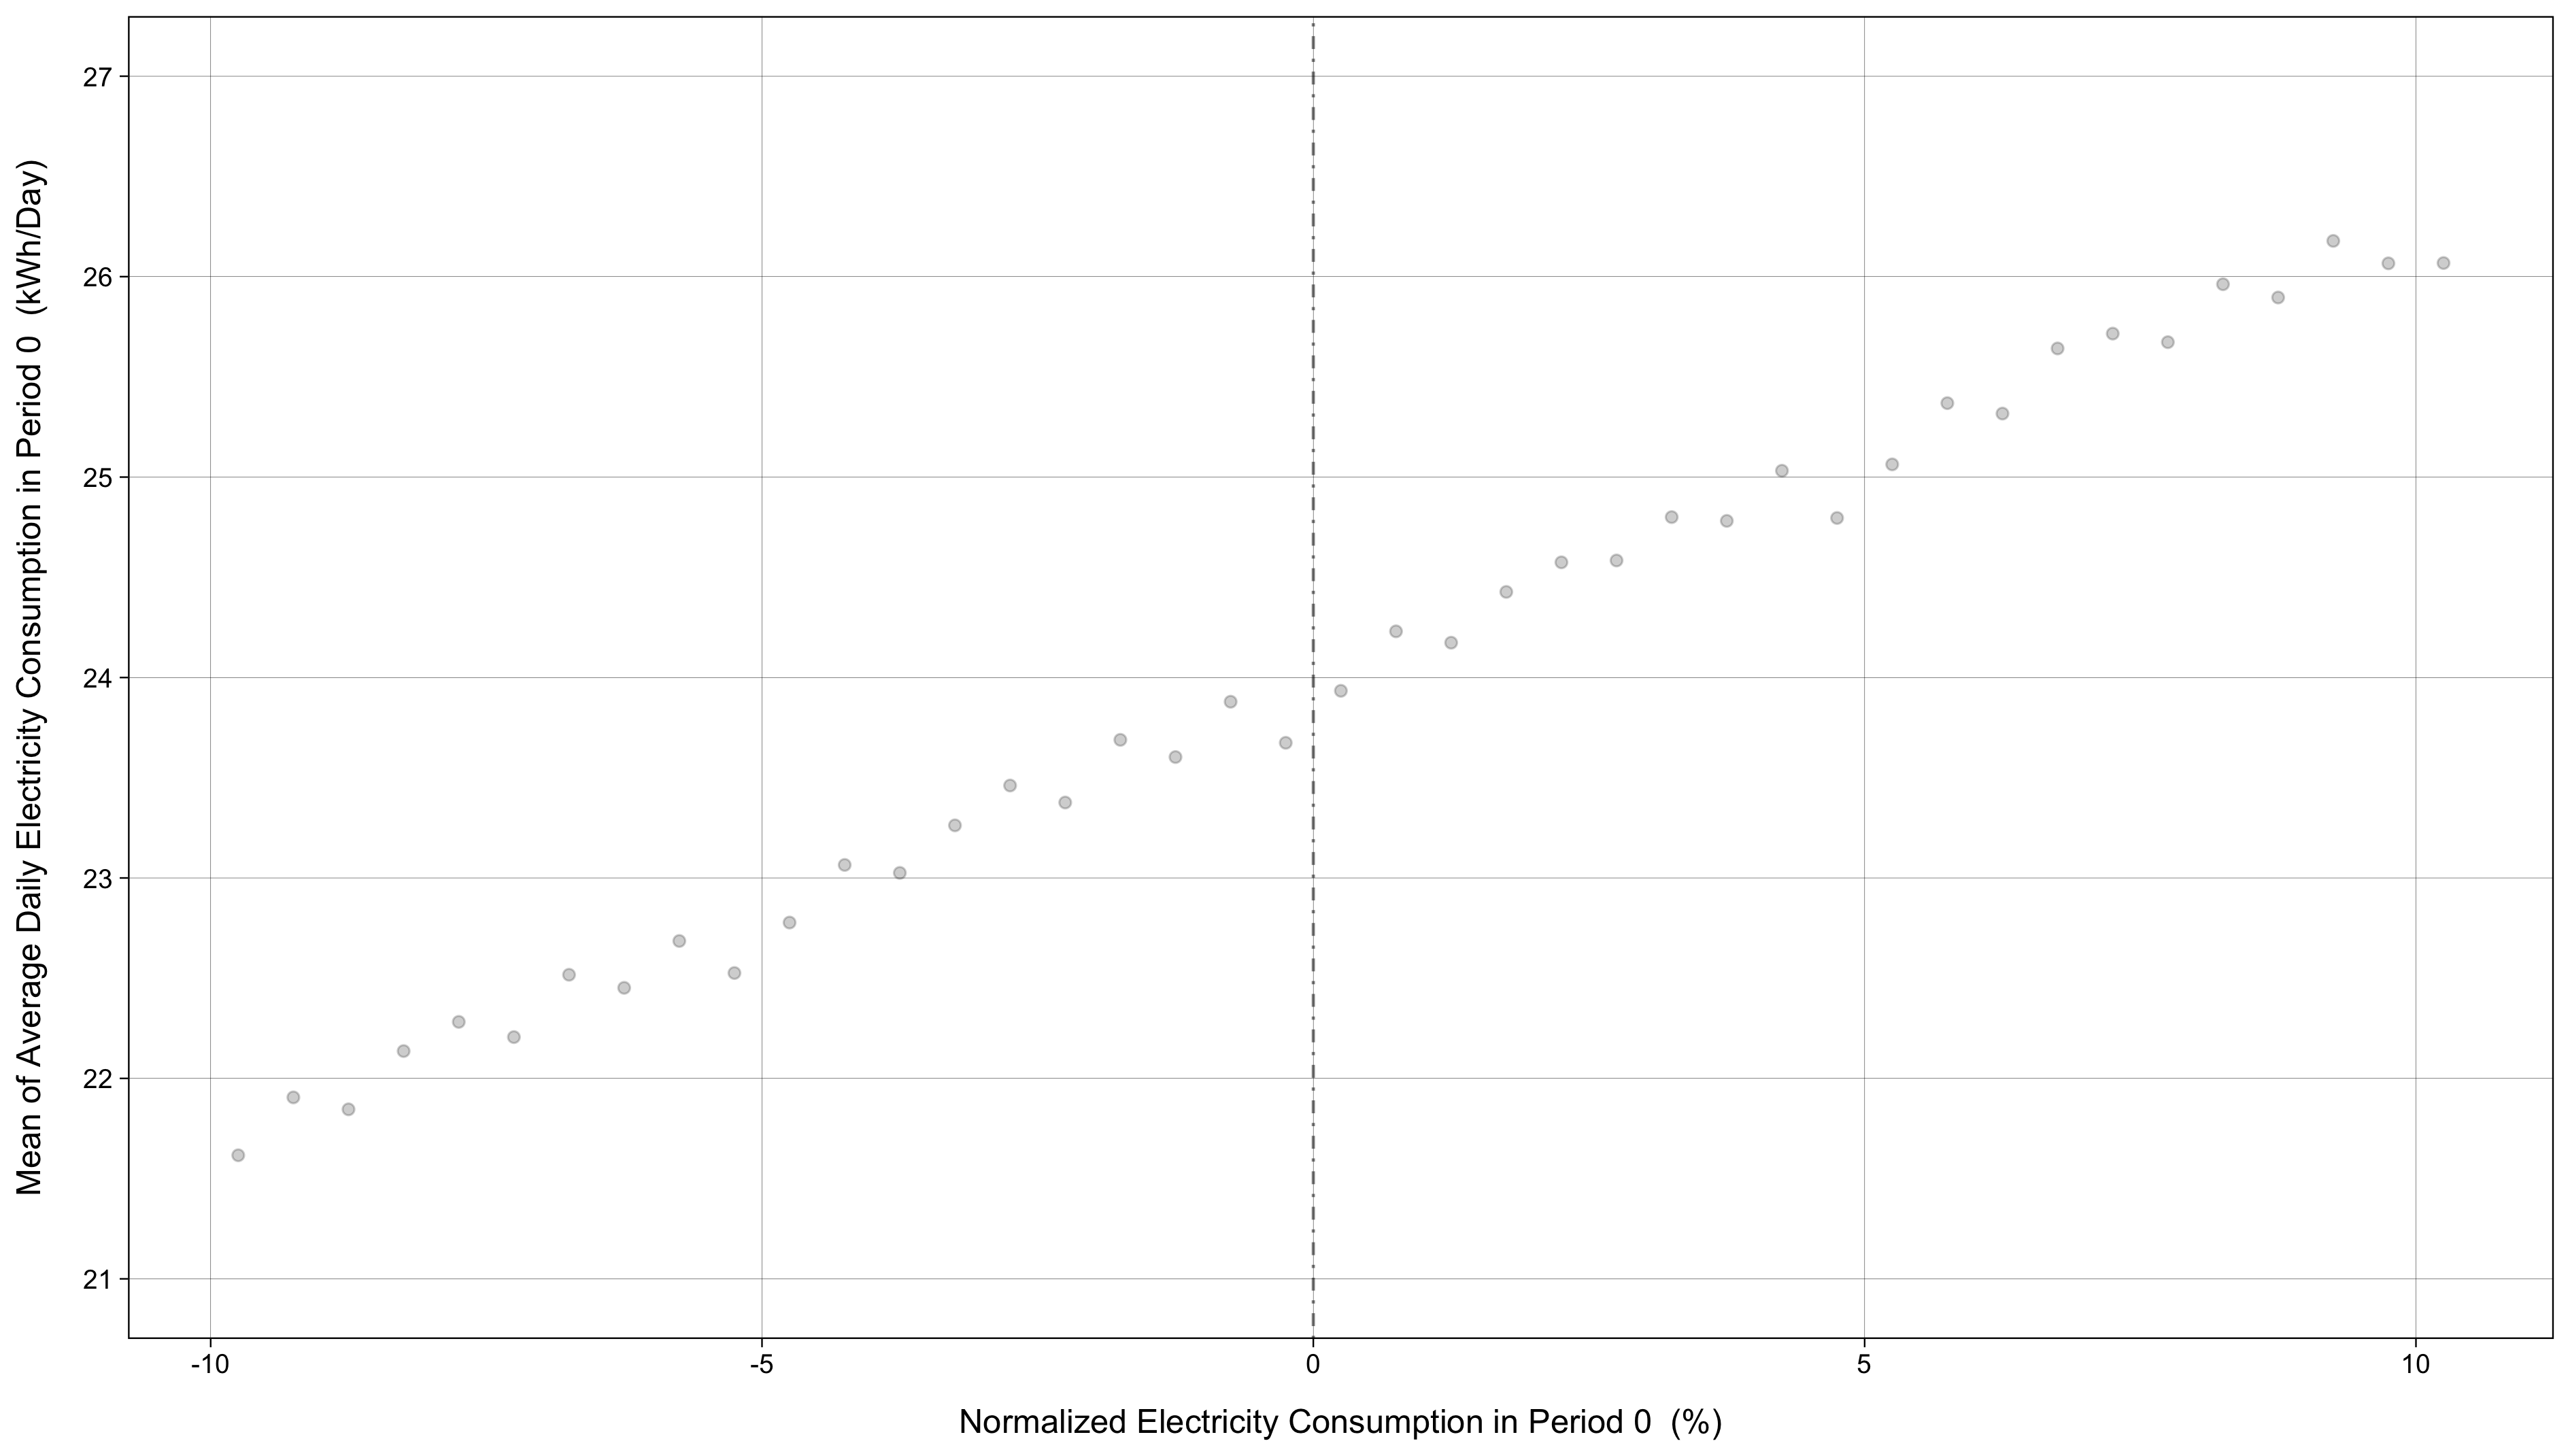
\includegraphics[scale = 0.115]{02_Chapter-1/00A_Figures/Figure_Average-Daily-Electricity-Consumption-in-Period-0-over-NC0.png}
        \caption{Mean of Average Daily Electricity Consumption in Period 0 over $\overline{NC}_{0}$}
        \caption*{
            {\small
            \textit{Note}: 
            In this figure, the scatter points correspond to the average daily electricity consumption in Period 0, calculated by binds with a bandwidth of 1\% of $\overline{NC}_{0}$. As can be seen, the average daily electricity consumption evolves smoothly around the cutoff point (i.e., $\overline{NC}_{0} = 0$). 
        }}
        \label{Figure:Average-Daily-Electricity-Consumption-in-Period-0-over-NC0}
    \end{figure}
}
Second, Figure \ref{Figure:Average-Daily-Electricity-Consumption-in-Period-0-over-NC0} demonstrates that households' average daily electricity consumption during Period 0 evolved smoothly around the lower cutoff point. This figure allows me, at a minimum, not to reject the assumption of local randomization around the base usage quantity, even though examining an observed covariate around the thresholds is not also a direct test for the validity of the assumption.




\section{Empirical Analysis and Results}
\label{C1-Section:Empirical-Analysis-and-Results}
\subsection{Household Responses to Lagged Marginal Prices in the RD Design}
\label{Sub-Section:Household-Responses-to-Lagged-Marginal-Prices-in-the-RD-Design}

\subsubsection{Econometric Model}
\label{Sub-Sub-Section:Econometric-Model}
Exploiting the sharp Regression Discontinuity (RD) design described earlier, I estimate the following econometric specification to measure how SMUD residential customers respond, in terms of their electricity consumption in a billing month (i.e., Period 1), to the discontinuous change in the marginal prices due to exceeding the lower base usage quantity in the previous billing month (i.e., Period 0):
\begin{equation}
\begin{split}
    ADC_{i, 1} \ 
    & = \ \beta_{0} \ + \ \beta_{1} \mathbb{1}[Treatment]_{i, 0} \ + \ f\left( \overline{NC}_{i, 0} \right) \ + \ \boldsymbol{X}'\boldsymbol{\alpha} \ + \ \delta_{ym} \ + \ \epsilon_{i, 1}
\end{split}
\label{Eq:RD-Econometric-Model}
\end{equation}

The dependent variable $ADC_{i, 1}$ is the average daily consumption by household $i$ in Period 1. $\widebar{NC}_{i, 0}$ corresponds to the running variable, household $i$'s normalized consumption in Period 0:
\begin{equation}
\begin{split}
    \overline{NC}_{i, 0} \ 
    & = \ kWh_{i, 0} \ - \ BUQ_{i, 0}
\end{split}
\label{Eq:Normalized-Consumption}
\end{equation}

where $kWh_{i, 0}$ and $BUQ_{i, 0}$ are, in Period 0, household $i$'s aggregate electricity consumption and the lower base usage quantity, respectively. The binary indicator variable $\mathbb{1}[Treatment]_{i, 0}$ is equal to 1 only if household $i$'s aggregate electricity consumption in Period 0 exceeded the lower base usage quantity:
\begin{equation}
\begin{split}
    \mathbb{1}[Treatment]_{i, 0} \ 
    & = \ 
    \begin{cases}
        \hspace{0.2cm} 0 \hspace{0.7cm} \text{if} \hspace{0.3cm} \overline{NC}_{i, 0} \ \leq \ 0 \\
        \hspace{0.2cm} 1 \hspace{0.7cm} \text{if} \hspace{0.3cm} \overline{NC}_{i, 0} \ > \ 0
    \end{cases}
\end{split}
\label{Eq:Treatment-Status-Determination-Rule}
\end{equation}

For $f\left( \widebar{NC}_{i, 0} \right)$, which is a continuous function of $\widebar{NC}_{i, 0}$, I utilize a variety of functional forms to show the robustness of my estimates. $\boldsymbol{X}$ are covariates, such as average daily Cooling Degree Days (CDDs) and average daily Heating Degree Days (HDDs). $\delta_{ym}$ is billing year-by-month fixed effects (FEs).\footnote{For a given billing observation, the mid-date of the observation determines the billing month-by-year.} The last term $\epsilon_{i, 0}$ is a stochastic error term. In this model, the coefficient of interest $\beta$ captures the treatment effect. I cluster the standard errors at the household ID as well as billing year-by-month levels to allow correlations across households in a given month.

In the specification, each household's average daily electricity consumption, instead of the aggregate consumption, in a billing cycle is utilized as the dependent variable. My sample contains household-level monthly billing records. But because of the fact that each billing month consists of a different number of days, I use each billing month's average daily consumption for my empirical analysis. For the same reason, average daily CDDs and HDDs are exploited in later analysis. 


\subsubsection{Regression Discontinuity Results}
\label{Sub-Sub-Section:Regression-Discontinuity-Results}
Table \ref{Table:RD-Results} summarizes the regression results of several alternate specifications for the bandwidth of 20\%. Column (1) reports estimates from the simplest RD specification without any control and FEs. Column (2) adds controls for households' cooling and heating needs, significantly driving household electricity consumption. In addition to those two controls, columns (3) and (4) use household and billing-year-by-billing-month FEs, respectively. Here, the estimated treatment effects are substantially smaller, suggesting that controlling for both household-specific and time-varying factors is important. Column (5) shows results from the specification with the controls and both FEs. The estimated treatment effect is a discontinuous reduction in households' average daily electricity consumption by 0.024 kWh (i.e., about 0.1\% of the average daily consumption). This estimate is statistically different from 0 at the 5\% level. Columns from (6) to (10) additionally include the interaction term between the binary indicator and running variables. Adding the interaction terms to the specifications has only minimal impact on the estimates.  

The identified reduction in household electricity consumption clearly demonstrates that households respond to lagged marginal prices. As discussed in Section \ref{Sub-Sub-Section:Regression-Discontinuity-Design}, the discontinuous increase in the marginal price at the lower base usage quantity was not followed by any change in the average price. Moreover, the households in my sample were able to notice the price jump only through their monthly bill statements, which were delivered a few days after the first day of the new billing month. Collectively, my estimates reveal an inefficiency stemming from households' responses to nonlinear electricity pricing because the lagged marginal price reflects their consumption history, not their contemporaneous consumption. In other words, under IBP, the untimely price signal drives households' electricity consumption. 

Importantly, the estimated treatment effect also indicates that SMUD residential customers overreacted to the lagged marginal price under nonlinear electricity pricing. The discontinuous change in the marginal price at the lower base usage quantity occurred in a billing cycle (i.e., in Period 0). And my estimates show that in the following billing cycle (i.e., in Period 1), the customers reduced their electricity consumption as a response to the price variation. Consequently, the sharp increase in the marginal price at the cutoff point in Period 0 affected all consumption, not the marginal one, in Period 1. That is, households excessively applied the lagged marginal price to every unit of electricity consumption. 

Inspired by \cite{Misunderstanding-Nonlinear-Prices_2020_(Shaffer)}, the estimates could be interpreted differently. The paper finds that a subgroup of less than 10\% of households was driving the seemingly overall response. If this is also true in my setting, then the measured decrease in household electricity consumption would be attributed to a subset of my sample. Let us suppose that there are two distinct types of SMUD residential customers: households over-responding to the lagged marginal price and those not responding to it.\footnote{Here, I do not consider the type of households that respond to the average price because the change in the marginal price at the threshold does not accompany any change in the average price.} My back-of-the-envelope calculation suggests that about 4\% of over-responders produce the estimated treatment effect.\footnote{In my rough computation, I exploit the price elasticity for the lagged marginal price provided in \cite{Do-Consumers-Respond-to-Marginal-or-Average-Price?-Evidence-from-Nonlinear-Electricity-Pricing_2014_(Ito)}.} Interestingly, this calculation parallels the finding in the paper. 



\subsubsection{Robustness Checks}
\label{Sub-Sub-Section:Robustness-Checks}
\noindent
\textit{\textbf{Regression Discontinuity Results for Different Bandwidths and Functional Forms}} --- 
Table \ref{Table:Robustness-Checks_BWs} summarizes the regression results for a set of different bandwidths. The estimated treatment effect for the households in a very narrow range from the lower base usage quantity (i.e., the households within the bandwidth of 5\%) is not statistically significant even at the 10\% level. Except for the bandwidth of 5\%, the treatment estimates range from $-$0.038 to $-$0.069 and statistically differ from zero at least at the 5\% level. The estimated treatment effect is almost identical for the bandwidths of 10\% and 15\%. For wider bandwidths falling between 20\% and 40\%, the magnitude of the estimated treatment effect increases and remains stable.\footnote{The number of observations increases with the size of the bandwidth exploited, except the two widest ones. The exceptions are because I drop observations crossing the higher base usage quantity to avoid picking up the effect of surpassing the higher cutoff point.} Interestingly, this table clearly shows that the wider the bandwidth employed, the larger the estimated treatment effect. In other words, the treatment estimates approach zero as I move even closer to the lower base usage quantity.

There are several possible explanations for this monotonic trend in the treatment effect. First, it may be more difficult or demanding for SMUD residential customers near the threshold to notice, from their monthly bill statements, that their electricity consumption in the previous billing month barely exceeded the lower base usage quantity, which in turn made them experience a discontinuous increase in the marginal price. Second, households whose electricity consumption just surpassed the cutoff point in a billing cycle could intentionally ignore the lagged price signal in the subsequent billing cycle. Some of them likely understood that their immediate electricity consumption was utterly irrelevant to the signal. And it is also possible that adjusting their electricity consumption pattern against the lagged marginal price during a whole billing month led to too much cost for some treated households very near the threshold compared to its benefit. Third, households near the lower base usage quantity may respond differently to the lagged marginal price compared to those farther from the threshold. Specifically, conditional on a given magnitude of the increase in the lagged marginal price, heavy electricity consumers could be more responsive to the price signal. 

Tables \ref{Table:Robustness-Checks_Functional-Forms_1st-and-2nd-Order-Polynomial-Models} and \ref{Table:Robustness-Checks_Functional-Forms_3rd-and-4th-Order-Polynomial-Models} present the regression results from other specifications having different functional forms. As illustrated in Figure \ref{Figure:The-Impact-of-the-Change-in-the-MP-due-to-Surpassing-the-Lower-BUQ}, a linear regression function seems highly reasonable on both sides of the threshold, even for broader bandwidth. The robustness of the results from the first four columns in Table \ref{Table:Robustness-Checks_Functional-Forms_1st-and-2nd-Order-Polynomial-Models} confirms that the linear approximation of the regression line does not induce considerable biases in my RD estimates. In addition, the RD estimates in the two tables suggest that for wider bandwidths, adding higher-order polynomials of the running variables is still reasonable for the estimates to be precise.


\par \vspace{0.5cm}
\noindent
\textit{\textbf{Falsification Test}} ---
Figure \ref{Figure:Robustness-Checks_Falsification-Tests} summarizes the results from falsification tests that examine treatment effects at two placebo cutoff points (i.e., at $-$30\% and 40\% of the normalized electricity consumption in Period 0 from the \textit{true} lower base usage quantity).\footnote{That is, the two false thresholds are at 70\% and 140\% of the normalized consumption in Period 0. Following the suggestion in \cite{Regression-Discontinuity-Designs_A-Guide-to-Practice_Imbens-and-Lemieux_2008}, I select those false cutoff points that are close to the median of the running variable on each side of the \textit{true} cutoff point.} In the falsification tests, I only use bandwidths less than the distance between a false threshold and the (actual) lower base usage quantity to avoid capturing some of the treatment effect. As clearly demonstrated, no estimate is different from zero at the 5\% level, suggesting that my RD design is valid. 




\subsubsection{Heterogeneity in Households Responses to Lagged Marginal Prices in the RD Design}
\label{Sub-Sub-Section:Heterogeneity-in-Household-Responses-to-Lagged-Marginal-Prices-in-the-RD-Design}
(...)



\subsection{Multi-Period Household Responses to Lagged Marginal Prices in the RD Design}
\label{Sub-Section:Multi-Period-Household-Responses-to-Lagged-Marginal-Prices-in-the-RD-Design}
(...)


\section{Policy Implications}
\label{C1-Section:Policy-Implications}
Utilizing the Regression Discontinuity (RD) design described in Section \ref{C1-Sub-Sub-Section:Regression-Discontinuity-Design}, I show that under Increasing-Block Pricing (IBP), residential electricity consumption responded to the lagged marginal prices, informed by their monthly bill statements. Before 2010, SMUD residential customers had no feasible way to know, in real time, how much electricity they had consumed since the beginning of a billing cycle, how much they paid for the marginal unit, and so on. In such a situation, it seems reasonable for them to use the available information---for example, the information contained in their monthly bills, which are delivered after several days after the last day of each billing cycle---as much as possible to make decisions about their electricity use. 

Nevertheless, it is undeniable that their electricity consumption responding to the lagged marginal price is suboptimal. As discussed, the marginal price to which households responded is not for the marginal unit in the current billing period but for the last unit in the previous one. In response to \textit{wrong} price signals, SMUD residential customers reduced their electricity consumption. Moreover, they applied the lagged price signals to all units of electricity consumption in a billing month, not just the last unit in a billing month. In other words, the \textit{informed} consumption decisions made by households, based on the lagged marginal prices, caused them welfare losses. 

The issue of household welfare losses due to their response to the discontinuous change in the lagged marginal prices suggests the importance of providing seemly price information in an appropriate manner. Many studies about various time-varying electricity pricing show that households changed their consumption behavior in response to the information about consumption and prices \citep{Dynamic-Pricing-of-Electricity-in-the-Mid-Atlantic-Region_Econometric-Results-from-the-Baltimore-Gas-and-Electric-Company-Experiment_Faruqui-et-al_2011, Knowledge-is-Less-Power_Jessoe-and-Rapson_2014, The-Effect-of-Information-on-TOU-Electricity-Use:An-Irish-Residential-Study_Pon_2017, Information-vs-Automation-and-Implications-for-Dynamic-Pricing_Bollinger-and-Hartmann_2020}. My empirical finding demonstrates that even under IBP, such information, though lagged, still plays a role in household electricity consumption. In this respect, providing household-specific as well as current price information to residential consumers, via text messages or app notifications, could encourage them to respond to \textit{true} price signals rather than lagged ones, which in turn avoids the negative impact on household welfare. Based on the dissipating effect of intermittently salient information discussed in \cite{Dynamic-Salience-with-Intermittent-Billing_Gilbert-and-Zivin_2014}, a high frequency of advising the latest tailored price information might maximize the behavioral change of households in electricity consumption.

My empirical results also suggest the significance of ensuring people understand the information provided correctly. Using an up-to-date machine learning technique, \cite{Peaking-Interest:How-Awareness-Drives-the-Effectiveness-of-Time-of-Use-Electricity-Pricing_Prest_2020} shows that the most critical driver of households' response to Time-Of-Use electricity pricing is their awareness of intraday price changes under the dynamic pricing. Given the empirical evidence suggested in \cite{Misunderstanding-Nonlinear-Prices_2020_(Shaffer)}, a subset of households in my sample may be driving the identified response to the lagged marginal prices.\footnote{For the households showing no response to the lagged price signals, there are two possible explanations: 1) they interpreted the signals correctly; or 2) they did not pay attention to it.} If this is the case, the household group perceived the variation in the lagged marginal prices informed by their monthly billing statements. However, their identified response to the lagged price signals clearly indicates that they misunderstood it as price information for right now. Herefore, in my empirical context, the result of my empirical analysis could suggest that it is crucial not only to get residential consumers to be aware of price changes, but also to get them to interpret the price signals correctly. 



\section{Conclusion}
\label{C1-Section:Conclusion}
In this paper, I examine how the electricity consumption of residential customers of SMUD responded to the marginal price informed through monthly bill statements under Increasing-Block Pricing (IBP). In a setting with a valid regression discontinuity design, my empirical analysis shows that households reduced their electricity consumption in response to the discontinuous price change in the marginal price in the immediately preceding billing cycle. In other words, the empirical results of my analysis reveal an inefficiency of IBP. At the same time, the interesting response demonstrates the potential to induce desired behavioral changes in household electricity consumption by providing appropriate price information regularly. On top of that, my RD results also indicate that the unit price of the highest block should be high enough to achieve the intended energy conservation by heavy electricity users. In conclusion, my research suggests implications for how IBP can be used more effectively without any welfare losses, especially in the case that transitioning toward time-varying electricity pricing, which is more efficient, is not feasible for some reason. 


% ------- Chapter 2 -------
\chapter{Prices Still Matter: How Households Adjust Their Consumption Behavior under Time-Of-Use Electricity Pricing}
\label{Chapter:Chapter-2}

\section{Introduction}
\label{C2-Section:Introduction}
These days many utilities are moving towards Time-of-Use (TOU) electricity tariff structures that raise the rate for peak-demand hours to the predetermined level, which does not vary across days. Many evaluations of experiments that assessed how residential consumers respond to TOU rates consistently document reductions in electricity consumption during peak hours. Those studies, however, do not examine how such reductions in household electricity consumption are achieved. In this research, to understand the mechanism of the demand reductions in detail, I decompose the decline in residential electricity consumption into two different sources of electricity savings: 1) electricity savings derived from the reduction in electricity consumption for temperature-control uses (e.g., cooling and heating), and 2) electricity savings from non-temperature-control uses (e.g., lighting, operating appliances, and cooking). Furthermore, instead of focusing only on the peak hours, my empirical analysis also covers intervals near the peak rate period (i.e., 2-hour-length pre- and post-peak intervals), in which the level of household electricity consumption changed a lot.

My study examines 30-minute interval residential electricity consumption data collected from a TOU pricing experiment conducted from July 2009 to December 2010 by the Commission for Energy Regulation (CER), the electricity and natural gas sector regulator in Ireland. Due to Irish households' widespread use of non-electric fuels for space and water heating, the sample utilized in the empirical analysis only includes meter readings from non-electric heating households in order to draw more universal policy implications from the empirical analysis. Using Difference-in-Differences (DID) strategy, I estimate the Average Treatment Effects (ATEs) of the TOU prices on household electricity consumption. To be specific, I measure how electricity savings from the TOU program vary with daily Heating Degree Days (HDDs). In addition, I also estimate how the savings alter with the magnitude of price changes in the peak rate period. By doing so, I find that around peak hours, the electricity savings stemming from the two distinct drivers of household electricity consumption (i.e., temperature-control and non-temperature-control uses) evolve differently depending on the point in time where electricity is consumed, daily HDDs, and the size of peak-hour price spikes.

The empirical analysis reveals that the TOU-price-causing variations in residential electricity demand are not restricted to the peak rate period. In addition to the consumption reductions during the peak rate period, my results show that participating households tend to cut their electricity consumption down before directly experiencing a price jump to the predetermined level. Moreover, such pre-adjustments are observed both from non-for- and for-heating electricity uses. 

From the detailed analysis, I also find that temperature-control-use-associated electricity savings are a nonlinear function of daily HDDs around peak hours. In other words, for a given peak-hour price jump, the impact of the TOU electricity tariffs on residential demand at an instant of time varies with daily HDDs. Specifically, the changes in household electricity consumption for heating show a U-shape profile over daily HDDs in the peak rate period, while those in the pre- and post-peak intervals do not emerge until daily HDDs are sufficiently sizable. 

The most absorbing finding from the empirical analysis is that households are highly responsive to the level of price changes in peak-demand hours. In the two-hour-length interval just before the peak-demand hours, the HDD-varying treatment effect on household electricity consumption for temperature-control uses is proportional to the size of the peak-demand-hours rate changes. On the other hand, the treatment effect on non-temperature-control-use-related electricity demand is inversely proportional to it. Interestingly, those relationships are flipped for the peak-rate-period electricity consumption. To be specific, the savings related to the for-heating use of electricity decrease as the price jumps in the peak-demand interval become more prominent, while the savings stemming from the electricity consumption for non-for-heating purposes is proportional to the jumps. Due to the opposite order of the magnitude of the demand reductions, the high sensitivity of household electricity consumption to the TOU tariffs around peak hours is masked. Indeed, this is precisely the result discussed in \cite{Peaking-Interest:How-Awareness-Drives-the-Effectiveness-of-Time-of-Use-Electricity-Pricing_Prest_2020}, which also utilizes the CER experiment datasets.\footnote{\cite{Peaking-Interest:How-Awareness-Drives-the-Effectiveness-of-Time-of-Use-Electricity-Pricing_Prest_2020} expresses the result as follows: ``Most of the overall response comes at the smallest price increase, with higher prices yielding strongly diminishing returns.''}

How households adapted their consumption behavior to the TOU tariff structures newly introduced can be deduced from those empirical findings above. Regarding the electricity consumption for non-temperature-control uses, the households assigned to the treatment group in the experiment simply reduced their demand around the peak rate period in lieu of reallocating it to off-peak hours. In other words, participating households reacted to the price jumps in peak demand hours, not through load-shifting but load-shedding. On the other hand, for-heating-associated electricity savings accompanied more complicated behavioral changes. Households adjusted their electricity consumption during the pre- and post-peak hours only when HDDs were large enough. And the reductions obtained from the pre-adjustment seem to lead to fewer savings in the following period (i.e., the peak rate period), especially on freezing days. 

Those findings disclose a veiled feature of TOU electricity pricing: day-varying effects on residential electricity savings. Let us suppose that the electricity savings obtained by adopting the TOU prices stem entirely from the reductions in non-temperature-control uses. In that case, intuitively, the magnitude of the savings does not vary across days. In other words, the amount of the savings does not depend on across-day temperature variations when residential demand for electricity peaks. However, my empirical results illustrate that on days with moderate heating needs, a sizable share of the electricity savings does stem from reductions in the use of electricity for temperature-control uses. Consequently, even though the TOU rates do not change across days, the tariff structures already induce substantial reductions in electricity consumption on typical winter days, in terms of daily HDDs, in Ireland. Therefore, on those days, the additional gains obtained by switching TOU prices to Real-Time Pricing (RTP) might be smaller than many economists have thought.\footnote{Under RTP, retail prices vary across not only hours of days but days according to contemporaneous generating costs.} 

The empirical results also provide new insights into the potential benefits of adopting even more dynamic price structures. As discussed earlier, the U-shaped evolving pattern of the temperature-control-use-associated electricity savings over daily HDDs in the peak rate period implies that TOU electricity pricing becomes less effective on days with extreme outside temperatures, on which the grid is most burdened, in turn, the most significant electricity savings are required. Nevertheless, considering that a high price change in the peak-demand hours not only prevents the temperature-control-use-driven electricity savings from disappearing but also produces more considerable non-temperature-control-use-related savings, allowing the peak-hour prices to rise by synchronizing it with daily HDDs would induce moderately more savings on high-demand days.

In addition, the identified gap, in terms of the most attainable for-heating-use-related electricity savings, between the lowest and the highest rate changes in the peak rate period suggests the potential gains from adopting automation technologies. As already discussed, the gap is likely a side effect of households' behavior change during the pre-peak interval. Hence, if it is possible to impede such changes in temperature-control-related electricity consumption from pre-peak to peak hours by exploiting an automation instrument, like an automated thermostat, more electricity savings can be achieved under TOU electricity pricing. 

To sum, the results from my empirical analysis extend the previous work by decoupling temperature-control-use-related electricity savings from the entire TOU-pricing-causing demand reductions. My results demonstrate that around peak hours, the savings from the two different sources sensitively vary according to the magnitude of the price changes in the peak rate period. That is, prices still matter under TOU tariff structures. Moreover, the day-varying electricity savings under TOU prices suggest a vital policy implication: shifting from TOU towards RTP-like pricing can improve residential electricity savings on extremely cold days. In addition, examining the electricity savings from two distinct sources, not in the peak rate period but around the peak rate period, enables unlocking the full benefits of TOU electricity pricing through the automation-technology-relevant policy implication. 



\section{Data}
\label{C2-Section:Data}
\subsection{Description of CER Experiment}
\label{SubSection:Description-of-CER-Experiment}
The Commission for Energy Regulation (CER), the regulator for Ireland's electricity and natural gas sectors, conducted the Smart Metering Electricity Consumer Behavior Trial (hereafter, the ``trial'') between July 2009 and December 2010. As part of the Smart Metering Project initiated in 2007, the trial's purpose was to assess the impact of various TOU tariff structures, along with different Demand-Side Management (DSM) stimuli, on residential electricity consumption. The CER carefully recruited households to construct a representative sample of the national population. Opt-in to the trial was voluntary. Participants received balancing credits not to incur any extra costs than if they were on the regular electric tariff (i.e., the flat rate of 14.1 cents per kWh). Also, they received a thank-you payment of 25 cents after pre- and post-trial surveys. All credits were distributed outside the treatment period to avoid unintended effects on participants' electricity consumption.\footnote{While the first balancing credit was paid at the end of the base period (i.e., in December 2009), the participants received the second one at the immediate month after the treatment period (i.e., in January 2011). And the after-survey payments were credited to their bill with the balancing credits.}

The households who voluntarily opt-in to the experiment were randomly assigned to control and treatment groups.\footnote{The optimal sample size for the trial was determined to be 4,300 participants in the design phase. In the allocation phase, 5,028 households were assigned to the control and treatment groups to consider participant attrition. The published CER experiment data include electricity consumption data only for 4,225 households.} Baseline electricity consumption data were collected during the second half of 2009 (i.e., July to December 2009), while the treatment period was from January through December 2010. All treated households received two kinds of treatments simultaneously: 1) one of four TOU tariff structures and 2) one of four DSM stimuli, described in detail later. In other words, there were 16 distinct treatment subgroups. The CER provided the treated with a fridge magnet and stickers to facilitate accustoming them to the TOU pricing schemes.\footnote{The fridge magnet and stickers outlined the timebands during which different prices were applied. Moreover, they were tailored for each tariff group.} On the contrary, the households allocated to the control group remained on the normal flat tariff.

The four TOU tariff structures had different prices during each of the three rate periods in a day. The day in the treatment period was divided into three periods: 1) peak rate period from 5:00 p.m to 7:00 p.m., 2) day rate period from 8:00 a.m. to 5:00 p.m. and from 7:00 p.m. to 11:00 p.m., and 3) night rate period from 11:00 p.m. to 8:00 a.m. As illustrated in Figure \ref{Figure:Time-Of-Use-Pricing-Structures}, the order of magnitude in rate changes during the peak rate period is the opposite of that for the rest of the rate periods. The reason for designing the tariff structures in such a way is to enable participating households to face similar energy bills on average when maintaining their electricity consumption pattern, regardless of the rate structures to which they were assigned. 

The four DSM stimuli differed in the degree or the frequency of feedback on each household's electricity usage information. The control group received their bills in the same cycle (i.e., bi-monthly). On the contrary, all households assigned to the treatment group received a detailed energy usage statement combined with their bill, including their detailed weekly usage, average weekly costs, tips on reducing electricity use, and comparisons to peer households. The first stimulus subgroup received a bill with a detailed energy statement bi-monthly, while the second subgroup received the documents every month. An electricity monitor, which displays their usage against their pre-set daily budget, was also provided for the households allocated to the third DSM stimulus subgroup. The last stimulus subgroup received an Overall Load Reduction (OLR) incentive. Under the OLR incentive, the households that reached their 10\% reduction target over the eight-month period beginning May 2010 were rewarded with 20 Euros.\footnote{A household's reduction target in electricity consumption was set based on the participant's actual usage during the first four months of the treatment period. And the households in the last DSM stimulus subgroup were updated on their progress with each bi-monthly bill.}



\subsection{Description of CER Experiment Data}
\label{SubSection:Description-of-CER-Experiment-Data}
The CER experiment dataset disseminated by the Irish Social Science Data Archive (ISSDA) consists of participating households' electricity consumption and survey data. 

Throughout the baseline and treatment periods, meter reads for residential participants were recorded in 30-minute intervals. The high granularity of the electricity consumption data generated from a well-designed experiment enables quantifying the energy savings when transferring to TOU electricity pricing for each of the three rate periods. 

The survey data contains participants' responses to more than 300 questions in pre- and post-trial surveys. The primary purpose of the two surveys was to gather trial-associated experiential and attitudinal feedback from the households. The surveys also included questions intended to collect residential participants' socio-demographic characteristics. In addition, questions about the physical attributes of their house were included in the surveys. 

My empirical analysis throughout this paper uses a longitudinal sample that consists of observations satisfying certain conditions only. First of all, the sample is constructed by including observations only for the second half of each experiment period.\footnote{I exclude the observations for the first half of the treatment period because there is no counterpart observation in the baseline period.} From this sample, I drop observations for non-holiday weekdays in the published electricity consumption data because the TOU rates were active just on those days. And then, only households that continuously exploited non-electric fuels for their space and water heating during the experiment periods (i.e., the baseline and the treatment periods) are preserved in the sample.\footnote{From the survey data, it is possible to find out what type of fuel each responding household used for each heating purpose during each period. \par
There are two reasons why only non-electric-heating households are exploited in the following empirical analysis. First, in Ireland, non-electric fuels, such as oil, gas, and solid fuels, fulfill most of the residential heating demand. Specifically, according to \cite{Heating-and-Cooling-in-Ireland-Today_SEAI_2022}, only 4\% of Irish households utilize electricity to heat their space and water. Therefore, with respect to fuels for heating in Ireland, the sample consisting of non-electric heating households only is representative. Second, as Figure \ref{Figure:Pre-and-Post-Treatment-Household-Average-Daily-Electricity-Consumption} demonstrates, even non-electric-heating households consumed more electricity as temperatures decreased. In other words, electricity is still essential for non-electric-heating households to warm their space or water. Hence, the sample, including non-electric-heating households only, is well aligned with one of the primary purposes of this research: to evaluate the impact of TOU pricing on for-heating-purpose residential electricity consumption separately.} Moreover, among the non-electric-heating households, those with unreliable meter reads are excluded from the sample.\footnote{To be specific, the residential participants who had no consumption for eight days or more are excluded from the sample. In addition, I drop the meter reads for the days when several participating households' consumption data were missed. \par
Although I utilize the sample satisfying the following criteria too for the empirical analysis, applying the criteria does not change the results: 1) Exclude the day immediately following the end of daylight-saving time due to noticeably different consumption levels in the same hours of the day; 2) Drop the observations for the last five days of the baseline and treatment periods because of extraordinarily high electricity demand on those days.} This process results in 4,096 households.

The control and treatment groups in the sample are largely balanced, as shown in Table \ref{Table:Summary-Statistics-and-Differences-in-Means-for-Treatment-and-Control-Groups}. Such indifferences between the two groups over many observables are consistent with previous studies examining the CER experiment dataset.\footnote{To check the balance between the control and treatment groups, \cite{Peaking-Interest:How-Awareness-Drives-the-Effectiveness-of-Time-of-Use-Electricity-Pricing_Prest_2020} employs a linear probability model, while a probit model is used in \cite{The-Effect-of-Information-on-TOU-Electricity-Use:An-Irish-Residential-Study_Pon_2017}. \par
Both papers point out that voluntary opt-in might cause bias in the estimated treatment effect. Refer to \textit{5.5.3 External Validity} in \cite{Peaking-Interest:How-Awareness-Drives-the-Effectiveness-of-Time-of-Use-Electricity-Pricing_Prest_2020} and \textit{5.1 Addressing Self-Selection} in \cite{The-Effect-of-Information-on-TOU-Electricity-Use:An-Irish-Residential-Study_Pon_2017}.}


\begin{table}
\caption{Treatment and Control Group Assignments}
\label{Table:Treatment-and-Control-Group-Assignments}
\end{table}

\begin{table}
\caption{Summary Statistics and Differences in Means for Treatment and Control Groups}
\label{Table:Summary-Statistics-and-Differences-in-Means-for-Treatment-and-Control-Groups}
\end{table}

\begin{figure}
\caption{Average Consumption by Hour of Day}
\label{Figure:Average-Consumption-by-Hour-of-Day}
\end{figure}



\subsection{Description of Weather Data}
\label{SubSection:Description-of-Weather-Data}
In this research, weather data are an essential element. The main interest of most TOU papers has been to measure how consumers respond to TOU prices or the heterogeneity in their responsiveness across different information stimuli. And the studies have focused on aggregate electricity consumption, consisting of consumption for a wide range of end-use types. Hence, those studies usually do not control temperature variations directly. For example, \cite{The-Effect-of-Information-on-TOU-Electricity-Use:An-Irish-Residential-Study_Pon_2017} and \cite{Peaking-Interest:How-Awareness-Drives-the-Effectiveness-of-Time-of-Use-Electricity-Pricing_Prest_2020}, which also exploited the CER experiment dataset, added weak-of-sample and month-by-year fixed effects (FEs) to their specifications, respectively, in order to control for variations in electricity usage due to seasonal changes. On the other hand, a novel approach adopted in this paper is to decompose household electricity consumption into two broad categories: non-temperature-control- and temperature-control-associated electricity consumption.\footnote{Details of the approach are discussed in Section \ref{Sub-subsection:Breakdown-of-Household-Responses-in-and-near-the-Peak-Rate-Period}.} Since the electricity consumption for temperature-control use is significantly driven by weather, particularly temperatures, it is necessary to link the 30-minute interval consumption data with reliable weather data that is of an appropriate level of resolution. 

I utilize average daily temperatures in my empirical analysis. More granular temperatures, like hourly temperatures, are not a dominant determinant of temperature-control-driven electricity consumption at a point in time. It is not easy to believe that households adjust their electricity consumption according to ever-changing outside temperatures elaborately and instantly.\footnote{Refer to \textit{3.4 Household Response to Dynamic Prices Exhibits Nontrivial Costs of Action That Impede Peak Reductions} in \cite{Household-Responses-to-Time-Varying-Electricity-Prices_Harding-and-Sexton_2017}.} Furthermore, as shown in Figure \ref{Figure:Average-Hourly-Electricity-Consumption-by-Time-of-Day}, their electricity demand is the lowest in the early morning, the coldest time of the day. Considering those two points, I measure the TOU-tariff-induced reductions in electricity consumption conditional on the average heating needs on a given day. 

I exploit hourly temperature data for the Dublin airport weather station, provided by Met \'{E}ireann, Ireland's National Meteorological Service, to compute average daily temperatures. There is no available location information in the published CER experiment dataset for privacy and security reasons. Therefore, it is impossible to match a participant's consumption data with the weather data of the closest weather monitoring station to him. But fortunately, in Ireland, temperatures do not vary much across areas for a given day. As demonstrated in Table \ref{Table:Correlations-in-Average-Daily-Temperatures-among-Weather-Stations}, the temperature correlations between the Dublin station and stations near densely populated cities are evident. Because of the close correlations, I use the mean daily temperatures obtained by averaging the Dublin airport station's hourly temperatures as the representative temperatures in the following analysis. 

Using the average daily temperatures, I calculate daily Heating Degree Days (HDDs). Instead of 65 degrees of Fahrenheit ($^{\circ}F$), a normal base temperature in the United States, 60$^{\circ}F$ is utilized to compute daily HDDs, according to \cite{The-Impacts-of-Climate-Change-on-Domestic-Natural-Gas-Consumption-in-the-Greater-Dublin-Region_Liu-and-Sweeney_2012}. Figure \ref{Figure:Distribution-of-Heating-Degree-Days-during-Experiment-Periods} shows that many days in the treatment period had lower average daily temperatures than the lowest one during the baseline period. The evolving pattern of temperature-control-driven demand for electricity on days with extreme temperatures could be significantly different under distinct rate structures---e.g., flat and TOU rates. If this is true, the lack of counterfactual consumption observations will cause bias in the measured impact of introducing TOU pricing on household electricity consumption. So, I drop observations for those days in the treatment period when constructing the sample to address the potential threat to the identification. 



\subsection{Empirical Strategy}
\label{SubSection:Empirical-Strategy}
\begin{figure}[!htbp]
\centering
\includegraphics[scale = 0.04]{03_Chapter-2/00A_Figures/Figure_For-Motivation_Daily-Consumption-with-Percentage-Changes_Base-only-the-Second-Half_Step-Size-2.png}
\caption{Pre- and Post-Treatment Household Average Daily Electricity Consumption}
\label{Figure:Pre-and-Post-Treatment-Household-Average-Daily-Electricity-Consumption}
\end{figure}

Figure \ref{Figure:Pre-and-Post-Treatment-Household-Average-Daily-Electricity-Consumption}, which shows household average daily electricity consumption over temperature and the pre and post differences in the consumption, clearly demonstrates the motivation of this research project.\footnote{An important feature also stands out from the figure: the minimum household electricity consumption occurred at around 60$^{\circ}F$. This phenomenon supports the setting of the reference temperature for calculating daily HDDs at the very level.} As illustrated in Panel A of the figure, household demand for electricity grew as the temperature decreased. In other words, in addition to temperature-insensitive electricity demand (i.e., for non-temperature-control uses), there was a sizeable demand for electricity for heating (i.e., for temperature-control use) in Irish households, which is highly responsive to temperature variations. In this research, I determine not only how much consumption changes, on average, in response to the time-varying tariffs but also how their impact varies across days with different temperatures. In other words, the dynamic-pricing-causing effects on heating and non-heating electricity uses are separately estimated to figure out the primary source of energy savings. As shown in the figure, households in the control group also consumed less electricity during the treatment period, especially on days with low temperatures, although their percentage reduction is smaller than that of the treated households.\footnote{In Panel A, non-treated households consumed more electricity during the baseline period, especially on days with higher heating needs. The fact that the total HDDs during the baseline period were generally greater than those during the treatment period for a given temperature bin could explain the phenomenon.} This suggests the necessity of employing an identification strategy that deals with the before and after differences in electricity consumption of households remained in the traditional tariff structure (i.e., a flat price of 14.1 cents for all hours). 

Because the CER experiment dataset primarily utilized in the following empirical analysis was generated from a carefully developed randomized controlled trial (RCT), in principle, the effect of the TOU tariffs on household electricity consumption can be measured simply through the difference in average usage between the two groups during the treatment period.\footnote{Because random assignment of participating households puts selection bias right, observed differences in electricity consumption between the control and treatment groups after introducing the TOU tariffs are only attributable to their differences in exposure to the time-varying electricity prices.} However, due to the non-trivial difference in electricity demand between the control and treatment groups during the baseline period, I follow the previous studies utilizing the same experiment and employ a difference-in-differences (DID) approach to estimate the electricity savings caused by the TOU pricing program.

I include the temperature as an explanatory variable directly in my econometric models. In the previous papers using the identical dataset, fixed effects (FEs) were utilized to control for time-varying factors that influenced household electricity consumption. Since those studies focused on quantifying how households responded, on average, to the TOU price regimes newly introduced, adding such FEs to their models served their research purpose. In other words, they did not need to explicitly model the relationship between temperature and household electricity consumption to estimate the average treatment effects (ATEs). However, a primary interest of this research is to understand how electricity savings vary with the temperature after shifting to TOU prices. Therefore, more direct controls rather than FEs, not sweeping out temperature variations across days, are required in my empirical analysis. For that reason, I extend the typical panel DID specification and allow the treatment effect to vary as a function of the daily average temperature.\footnote{Under three identifying assumptions, applying the DID strategy to measure energy savings obtained from adopting the TOU prices makes sense. First, the parallel trend assumption is required for the DID estimator. Considering that the 30-minute interval meter reads for participating households were collected from a trial, the assumption means that the pre-treatment-period load profile for the treated households should be very similar to that for the non-treated households. FIGURE A showing average within-day load profiles for the two groups during the baseline period supports the plausibility of the parallel trend assumption. In addition, the electricity consumption profile for the control group illustrated in FIGURE B, which smoothly evolved over the entire experiment period although heavily fluctuated day to day, suggests its high reliability as a counterfactual under the assumption. \par
The second identifying assumption necessary for the plausibility of the identification strategy employed is the assumption of common temporal shocks. This assumption implies that a treatment-status-irrelevant unexpected event occurring at the same time as or following the deployment of the dynamic prices should have the same impact on both the control and treatment groups. Although the common shocks assumption cannot be tested directly, the similar trends in electricity demand profiles for the control and treatment groups shown in FIGURE B support the assumption required for the DID approach. \par
Third, the stable unit treatment value assumption (SUTVA) must hold too. The SUTVA requires that introducing TOU prices did not affect the electricity consumption of the untreated households. That is, the SUTVA allows no spillovers. During the recruitment process, the locational distribution of the participating households was aligned with that of the total Irish population to construct a representative sample of the national population. Because only a few thousand households scattered geospatially participated in the nationwide experiment, it is unlikely that the treated households influenced the households allocated to the control group. This again supports the SUTVA required under the DID identification strategy.} That is, I estimate the ATEs of the dynamic prices on household electricity demand by exploiting the within-household electricity consumption changes across not only periods but temperatures.\footnote{The attrition rate during the RCT was about 20\%. The main reasons for participant attrition were changes in tenancy and supplier. Due to the imperfect compliance, the estimates must be interpreted as local average treatment effects (LATEs). However, according to CER (2011), attrition was unlikely to be associated with the RCT. Furthermore, the level of attrition varied only marginally across treatment status.}

\begin{figure}
\caption{Summary Statistics and Differences in Means for Treatment and Baseline Periods}
\label{Figure:Summary-Statistics-and-Differences-in-Means-for-Treatment-and-Baseline-Periods}
\end{figure}




\section{Empirical Analysis and Results}
\label{C2-Section:Empirical-Analysis-and-Results}
\subsection{Household Average Responses to Time-Of-Use Electricity Pricing}
\label{Subsection:Household-Average-Responses-to-Time-Of-Use-Electricity-Pricing}
\subsubsection{Half-hourly Average Treatment Effects}
\label{Sub-subsection:Half-hourly-Average-Treatment-Effects}
Utilizing a panel DID identification strategy, I first measure the impact of the TOU prices on 30-minute-interval household electricity consumption. To obtain the Average Treatment Effect (ATE) for each half-hour interval, I estimate the following specification:
\begin{equation}
\begin{split}
    \textit{kWh}_{itw} \ 
    & = \ \beta_{w} \mathbb{1}\big[ \text{Treatment \& Post} \big]_{it} \ + \ \alpha_{iw} \ + \ \gamma_{tw} \ + \ \delta_{m} \ + \ \epsilon_{itw}
\end{split}
\label{Eq:Model-Specification_Half-Hourly-Average-Treatment-Effects}
\end{equation}
The term $kWh_{itw}$ is the electricity consumption by household $i$ on the day $t$ during the half-hourly time window $w$. The indicator variable $\mathbb{1}\big[ \text{Treatment \& Post} \big]_{it}$ is equal to 1 only if household $i$ is in the treatment group and the day $t$ is in the treatment period. The terms $\alpha_{iw}$, $\gamma_{tw}$, and $\delta_{m}$ are household-by-half-hourly-interval, day-of-sample-by-half-hourly-time-window, and month-of-year fixed effects, respectively. In the specification, the point estimates of $\beta_{w}$, representing the ATE for each 30-minute interval $w$, are the parameters of interest. I cluster the standard errors at the household and the day of experiment levels to correct for serial correlation.

\afterpage{
    \begin{figure}
        \centering
        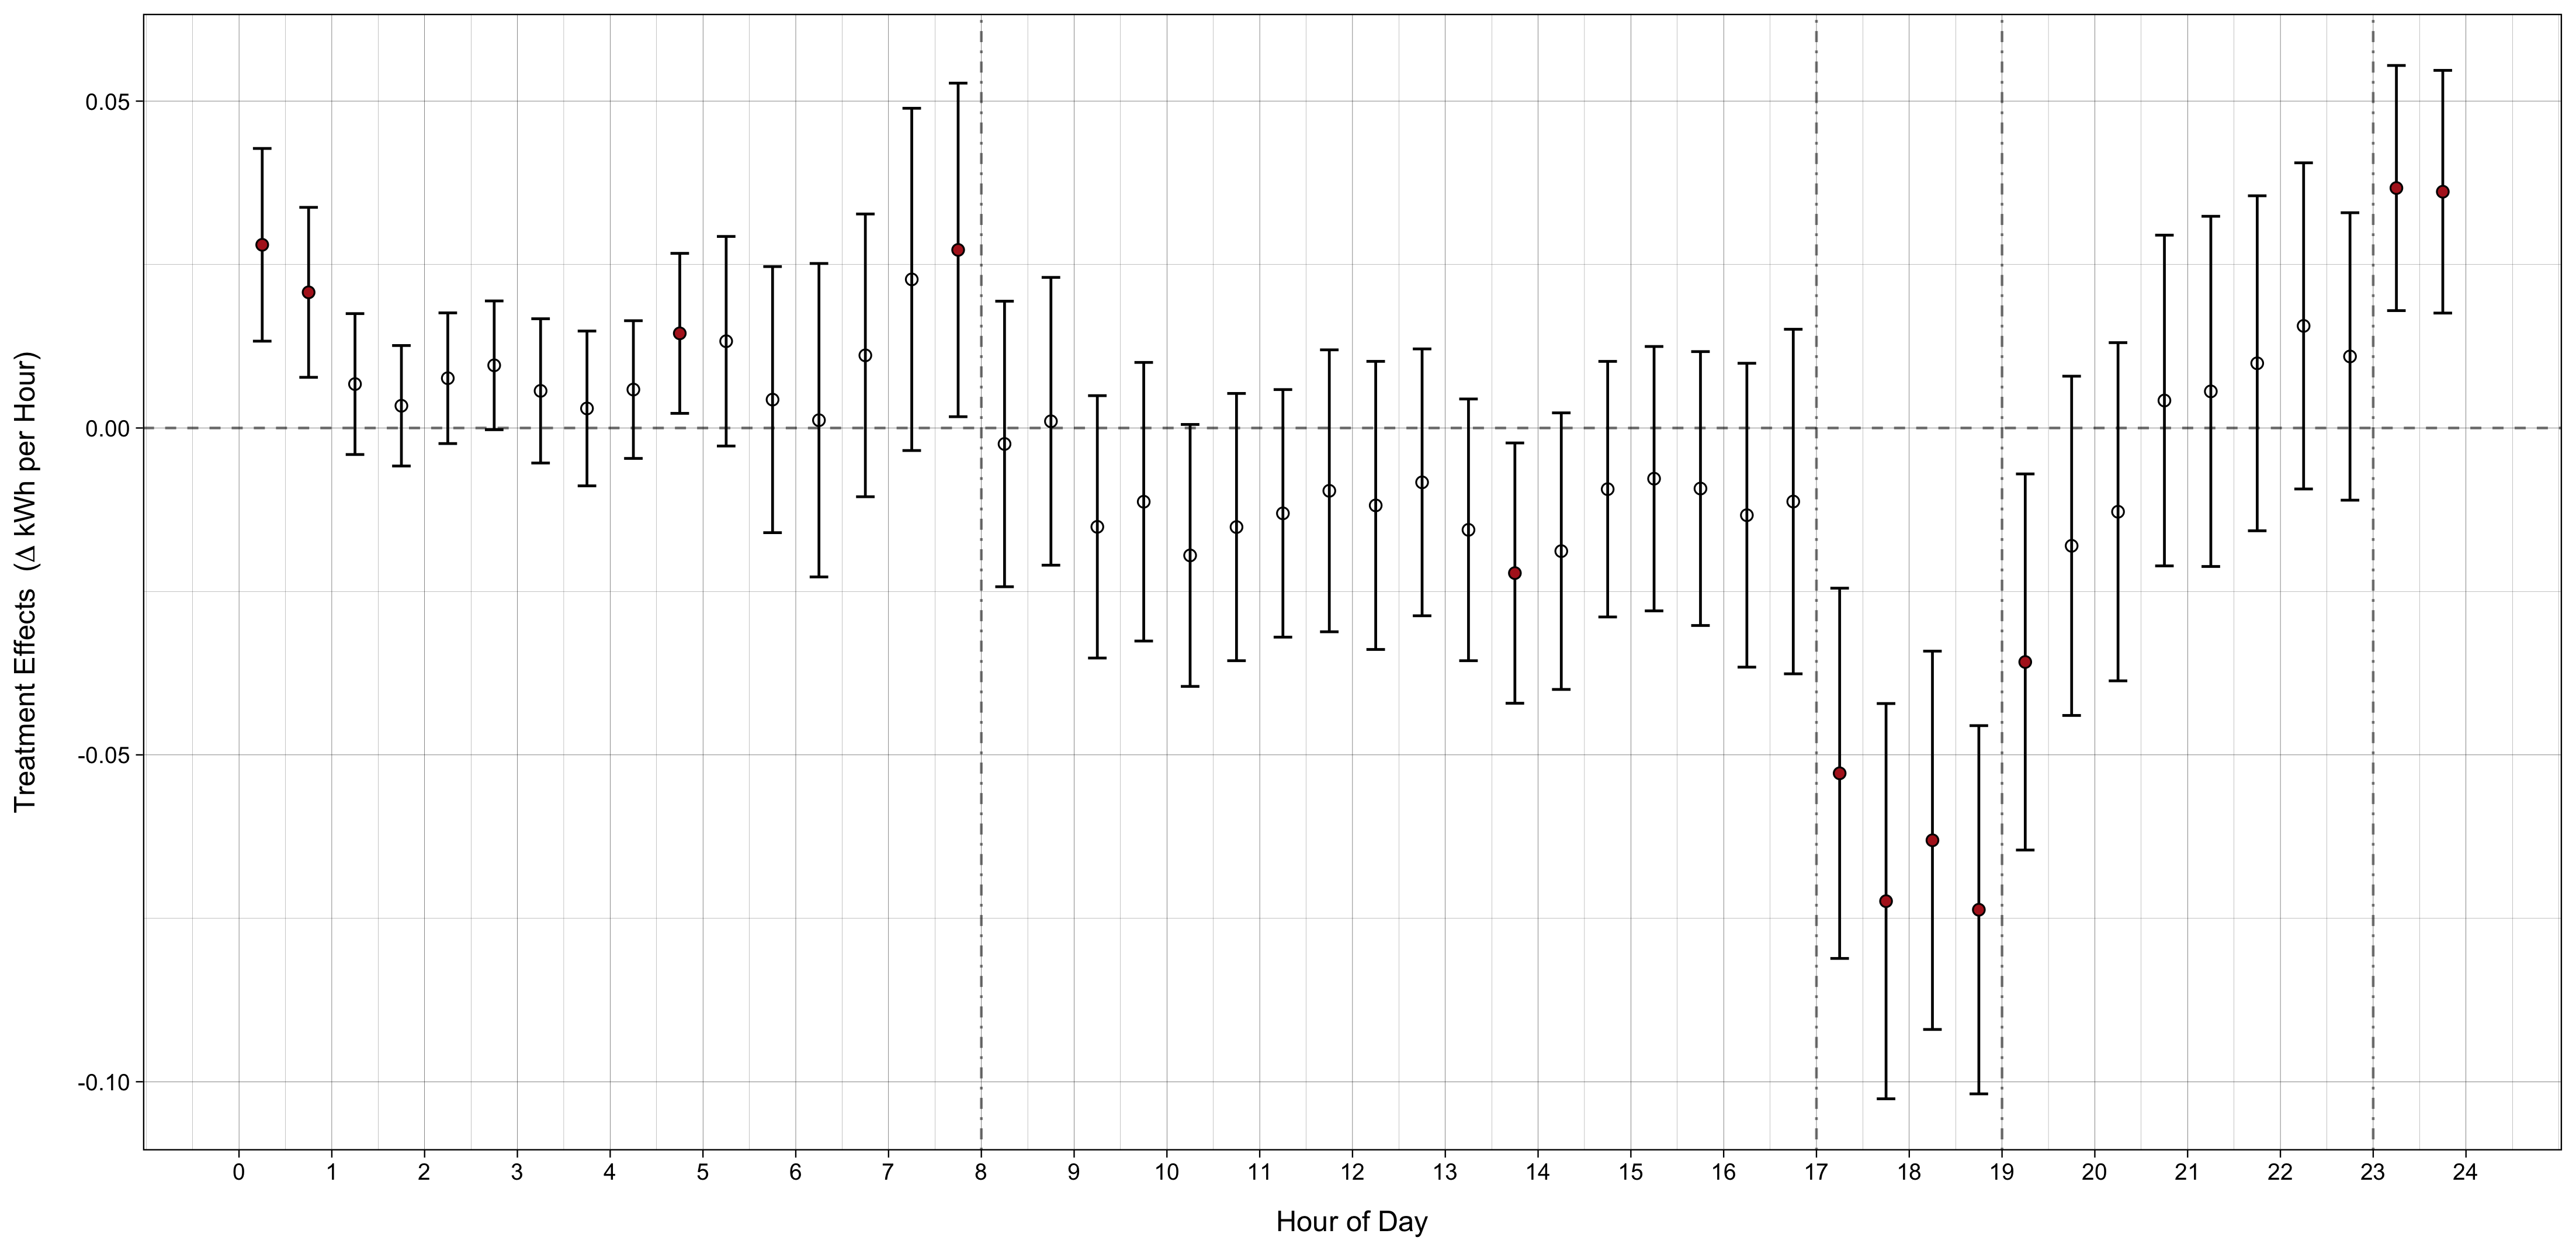
\includegraphics[scale = 0.10]{03_Chapter-2/00A_Figures/Figure_Time-Profile-of-Half-Hourly-ATEs.png}
        \caption{Half-hourly Average Treatment Effects}
        \caption*{
            {\small
            \textit{Note}: This figure depicts the time profile of half-hourly average treatment effects with 95\% confidence intervals. Standard errors are clustered at the household and date levels to adjust for serial correlation. As clearly illustrated, the treated households significantly reduced their electricity consumption during peak hours. A more interesting phenomenon is that they reduced their electricity consumption in hours leading up to and following the peak rate period, during which the applicable unit rate was lower than the flat rate in the baseline period, even though most of the estimated treatment effects are statistically insignificant in those hours. 
        }}
        \label{Figure:Half-Hourly-Average-Treatment-Effects}
    \end{figure}
}
Figure \ref{Figure:Half-Hourly-Average-Treatment-Effects} summarizes the estimated ATEs in the form of a time profile. As already demonstrated in \cite{Peaking-Interest:How-Awareness-Drives-the-Effectiveness-of-Time-of-Use-Electricity-Pricing_Prest_2020}, peak hours (i.e., from 5:00 p.m. to 7:00 p.m.) show dominant electricity savings. The figure also demonstrates reductions in household electricity consumption not only in most of the meter readings prior to the peak rate period but also in three successive meter readings right after the period, even though the reductions, with two exceptions, are not statistically significant. The insignificant reductions in household electricity consumption are interesting because TOU prices in off-peak hours (i.e., prices in the night and day rate periods) were lower than the flat rate in the baseline period. The counterintuitive changes might indicate that households preemptively adjusted their consumption behavior to avoid the incident of paying higher prices. In other words, the peak-hour price increases under the TOU program were likely to cause some spillover effects in the hours leading up to and following the peak rate period. To explore whether households responded to the TOU program outside of the peak rate period as well or not, in the following empirical analysis, I will also pay attention to the off-peak hours, particularly the hours surrounding the peak rate period.



\subsubsection{Hourly Average Treatment Effects in and near the Peak Rate Period}
\label{Sub-subsection:Hourly-Average-Treatment-Effects-in-and-near-the-Peak-Rate-Period}
Estimating by-tariff-group ATEs in and near the peak rate period allows understanding how the relationship between the degree of change in household electricity consumption and the magnitude of a peak-demand-hour price increase evolves in and near the peak rate period.\footnote{In this paper, the effects of four different information stimuli on household electricity consumption are not of interest. \cite{The-Effect-of-Information-on-TOU-Electricity-Use:An-Irish-Residential-Study_Pon_2017} studied the effects in detail using the same datasets.} To do so, I run the following regression for each of the four tariff groups:
\begin{equation}
    \textit{kWh}_{ith} \ 
     = \ \beta_{p} \mathbb{1}\big[ \text{Treatment \& Post} \big]_{it} \ + \ \alpha_{iw} \ + \ \gamma_{tw} \ + \ \delta_{m} \ + \ \epsilon_{ith}
\label{Eq:Model-Specification_Hourly-Average-Treatment-Effects}
\end{equation}

Excepting the dependent variable and the parameter of interest, the econometric model above is the same as (\ref{Eq:Model-Specification_Half-Hourly-Average-Treatment-Effects}). Specifically, the response variable $kWh_{ith}$, which means the electricity consumption by household $i$ on the day $t$ during the hour of the day $h$, is utilized due to its better accessibility in interpretation. The point estimates of $\beta_{p}$ indicate the ATE for each of the three intervals included in rate period $p$. Table \ref{Table:Hourly-Average-Treatment-Effects-in-and-near-the-Peak-Rate-Period} summarizes the regression results.

The measured ATEs for the peak rate period re-confirm the finding provided in \cite{Peaking-Interest:How-Awareness-Drives-the-Effectiveness-of-Time-of-Use-Electricity-Pricing_Prest_2020}.\footnote{See Figure 6 in \cite{Peaking-Interest:How-Awareness-Drives-the-Effectiveness-of-Time-of-Use-Electricity-Pricing_Prest_2020}.} The table clearly shows that within-household aggregate demand for electricity during the peak rate period declined, with a significance level of 0.01, due to the deployment of TOU pricing. However, based on the point estimates for the four tariff groups, it is unclear whether an incremental change in peak-rate-period price increase induces a statistically meaningful additional change in household electricity consumption or not. 

%\begin{landscape}
\input{03_Chapter-2/00B_Tables/Table_ATEs_Hourly-in-and-near-the-Peak-Rate-Period.tex}
%\end{landscape}
%\clearpage
To quantify how residential consumers responded to the TOU program in off-peak hours close to the peak rate period, I also estimate ATEs in periods of two hours before and after the peak rate period (i.e., in pre- and post-peak periods). Interestingly, the table also demonstrates that in the pre- and post-peak periods, the implementation of the TOU tariff structures resulted in reductions in household electricity consumption, which are statistically different from zero, even though TOU prices were lower than the flat rate of 14.1 cents per kWh.\footnote{Even insignificant point estimates (i.e., point estimates for Tariff Groups C and D in the pre-peak interval and Tariff Group C in the post-peak interval) have negative values.} The reductions in both periods surrounding the peak hours suggest that the impact of the price increases in the peak rate period overtook the impact of the price drops in each off-peak period. Therefore, in the following empirical analysis, I will focus on linking household electricity consumption in the pre- and post-peak periods with the price increases in the peak rate period, instead of the price decreases in those off-peak periods. 



\subsection{Breakdown of Household Responses to Time-Of-Use Electricity Pricing}
\label{Subsection:Breakdown-of-Responses-to-Time-Of-Use-Electricity-Pricing}
\subsubsection{Breakdown of Household Responses in and near the Peak Rate Period}
\label{Sub-subsection:Breakdown-of-Household-Responses-in-and-near-the-Peak-Rate-Period}
Figure \ref{Figure:Average-Daily-Electricity-Consumption} indicates the limitations of focusing on aggregate electricity consumption, as many studies have been doing. The figure clearly shows that aggregate household electricity consumption increases as the weather becomes colder in Ireland. Intuitively, the negative correlation between them can be mainly attributable to for-heating electricity consumption, which strongly depends on outdoor temperatures. It is a fact that aggregate residential electricity consumption also includes another type of electricity consumption: electricity consumption that is irrelevant to temperature variations, such as consumption for lighting. Those two broad categories of electricity consumption could react differently to TOU electricity pricing. Electricity consumption for heating can be transferred to a different time of the day (e.g., from 6 p.m. to 4 p.m. to avoid a higher unit price under the TOU tariff structures). On the other hand, electricity consumption for lighting is time sensitive. Due to the difference in the costs of relocating or changing electricity consumption, it is possible that the two channels of household electricity consumption respond to TOU electricity pricing in different ways. Therefore, using aggregate electricity consumption to examine households' responses to the time-varying price scheme enables me to access only the aggregated response. 

Considering the discussion above, I decompose household electricity consumption into two broad categories---non-temperature-control-driven and temperature-control-driven electricity consumption---and examine how each category of electricity consumption responds to the introduction of the TOU tariff structures. The temperature-control-related electricity consumption here means using electricity to satisfy home heating needs (e.g., to warm up space or water). So, the use of electricity for heating strictly depends on each day's weather conditions, especially temperatures. Naturally, the non-temperature-control-associated electricity consumption makes up the rest. 

I exploit daily Heating Degree Days (HDDs), which imply overall heating needs on a given day, to isolate the temperature-control-driven consumption from aggregate household electricity consumption. Because only aggregate metering data is available from the CER experiment dataset, there is no clue allowing me to classify household electricity consumption into two distinct categories in the dataset. To address this challenge, I presume that the portion of household electricity consumption that fluctuates according to daily HDDs is temperature-control-driven electricity consumption. Therefore, the electricity consumption for temperature-control use is additional consumption that appears only on days with non-zero daily HDDs due to household heating needs.

To break down household responses to the TOU program around the peak rate period, I exploit the following DID-style spline regression model:\footnote{The control group's less percentage changes on freezing days, which are illustrated in Figure (\ref{Figure:Pre-and-Post-Treatment-Household-Average-Daily-Electricity-Consumption}) substantiate the use of the DID-style spline regression model in \ref{Eq:Model-Specification_Breakdown-of-Hourly-Average-Treatment-Effect}.}:
\begin{equation}
\small
\begin{split}
    kWh_{ith} \
    & = \ \beta_{1} HDD_{t} \ + \ \beta_{2} HDD_{t}^{*} \\
    & \hspace{0.7cm} + \ \big( \beta_{3} \ + \ \beta_{4} HDD_{t} \ + \ \beta_{5} HDD_{t}^{*} \big) \mathds{1}[\text{Treatment}]_{i} \\
    & \hspace{0.7cm} + \ \big( \beta_{6} \ + \ \beta_{7} HDD_{t} \ + \ \beta_{8} HDD_{t}^{*} \big) \mathds{1}[\text{Post}]_{t} \\
    & \hspace{0.7cm} + \ \big( \beta_{9} \ + \ \beta_{10} HDD_{t} \ + \ \beta_{11} HDD_{t}^{*} \big) \mathds{1}[\text{Treatment \& Post}]_{it} \ + \ \kappa_{dw} \ + \ \epsilon_{ith} 
\end{split}
\label{Eq:Model-Specification_Breakdown-of-Hourly-Average-Treatment-Effect}
\end{equation}
Like (\ref{Eq:Model-Specification_Hourly-Average-Treatment-Effects}), the dependent variable $kWh_{ith}$ is the electricity consumption by household $i$ on the day $t$ during the hour of the day $h$. In this model, the full set of fixed effects in (\ref{Eq:Model-Specification_Hourly-Average-Treatment-Effects}) has been superseded by two indicator variables---the first indicator variable $\mathbb{1}[\text{Treatment}]_{i}$ has the value of 1 if household $i$ is assigned to the treatment group, and the second indicator variable $\mathbb{1}[\text{Post}]_{t}$ equals 1 when the day $t$ is in the treatment period. Although using the fixed effects as in (\ref{Eq:Model-Specification_Hourly-Average-Treatment-Effects}) does not affect the treatment effects of interests, which is expected given the randomization, replacing them with the indicator variables allows for the interpretation of the average consumption by the treatment group to be more straightforward.\footnote{Added indicator variables instead of various fixed effects also enables an easier graphical summary of the regression results.} The model also includes interaction terms between HDD-relevant terms and those indicator variables. In the econometric model, $HDD_{t}$ means the daily heating degree days on the day $t$. And $HDD_{t}^{*}$, which is required to introduce nonlinearity in HDD-associated response to TOU pricing, is mathematically defined as follows:
\begin{equation}
HDD_{t}^{*} \ = \ (HDD_{t} - Knot) \ \times \ \mathbb{1}[HDD_{t} > Knot],
\end{equation}
where $Knot$ is a reference value at which the slope of the predicted line starts to change. For $Knot$, I utilize the value of ten in the following regression analysis because the median values of daily HDDs in the baseline and treatment periods are ten. The term $\kappa_{dw}$ is day-of-week-by-half-hourly-time-window fixed effects. 

The primary coefficients of interest in (\ref{Eq:Model-Specification_Breakdown-of-Hourly-Average-Treatment-Effect}) are $\beta_{9}$, $\beta_{10}$, and $\beta_{11}$. The three coefficients show how much electricity consumption changes in the households assigned to the treatment group changed after implementing the TOU program compared to those in the control group. To be specific, $\beta_{9}$ demonstrates the change in residential electricity consumption for non-temperature-control use. Both $\beta_{10}$ and $\beta_{11}$ collectively represent the change in the amount of electricity consumed to meet household heating needs at given daily HDDs. 

Using the point estimates of the three coefficients of interest provided in Table \ref{Table:Breakdown-of-Hourly-ATEs}, I graphically summarize the predicted change in each of the two channels of electricity consumption in Figure \ref{Figure:Breakdown-of-Hourly-ATEs-in-the-Peak-Rate-Period}. Regarding the change in electricity consumption for non-temperature-control use, the table and figure clearly show that the treated households significantly reduced their consumption when they were subject to peak-hour prices (i.e., in the peak rate period). Their non-temperature-control-driven electricity consumption also decreased in the pre- and post-peak periods, albeit noisy and relatively smaller in magnitude than the peak-hour changes. 

The change in temperature-control-associated electricity consumption occurred as well in all three two-hour periods, but its evolving pattern over daily HDDs was quite different in each period. Specifically, the impact of TOU pricing on residential electricity consumption for heating was U-shaped in the peak rate period. In contrast, in the hours before and after the peak period, the TOU intervention altered the electricity use for heating only on the coldest days (i.e., only when daily HDDs were sufficiently large). In other words, from the figure, it is evident that the change originating from temperature-control-related electricity consumption was a nonlinear function of daily HDDs in all three periods.

Specification (\ref{Eq:Model-Specification_Breakdown-of-Hourly-Average-Treatment-Effect}) is also utilized to examine, for the peak rate period, the relationship between the degree of a price increase in that period and the change in electricity consumption. The by-tariff-group estimates of the coefficients of interest are also presented in Table \ref{Table:Breakdown-of-Hourly-ATEs}. As shown in the table, on the whole, the reduction stemming from electricity demand for non-temperature-control use tends to be proportional to the size of price growth in peak hours, even though the point estimate for Tariff Group C is an exception. Therefore, the marginally diminishing effects of TOU pricing, discussed in \cite{Peaking-Interest:How-Awareness-Drives-the-Effectiveness-of-Time-of-Use-Electricity-Pricing_Prest_2020}, seem not to be championed by my point estimates. To be specific, while the aggregate electricity consumption during the peak rate period does not sensibly respond to incremental changes in the peak-hour price, the amount of electricity used for non-temperature-control purposes in the peak rate period does respond meaningfully to the marginal changes in the peak price. And the two estimates associated with temperature-control-driven electricity consumption (i.e., $\hat{\beta}_{10}$ and $\hat{\beta}_{11}$) are statistically significant only for the case of the smallest price increase (i.e., only for Tariff Group A).\footnote{In case of Tariff Group D, only $\hat{\beta}_{11}$ is statistically significant.} 

Altogether, those results imply two interesting points. First, the two distinct types of electricity consumption showed widely different responses to TOU prices in all three periods of two hours. Second, the measured reductions in non-temperature-control-related electricity consumption seem highly sensitive to the magnitude of a price increase in the peak rate period. Inspired by those implications, I formulate the resulting variations in household electricity consumption as a linear function of the magnitude of a rate change in peak-demand hours in the following section.



\subsubsection{Household Responses as a Linear Function of Price Changes}
\label{Sub-subsection:Household-Responses-as-a-Linear-Function-of-Price-Changes}
To fully understand how residential consumers adjust their consumption behavior as a set of reactions to the price changes under the TOU program, it is necessary to explicitly examine, for each of the three periods (i.e., the pre-peak, peak, and post-peak periods), the relationship between the size of a price increase in the peak rate period and the changes in the two distinct categories of household electricity consumption. For that reason, I quantitatively determine the relationship by utilizing the following econometric model:
\begin{equation}
\small
\begin{split}
    kWh_{ith} \ 
%    & = \ \beta_{1} HDD_{t} \ + \ \beta_{2} HDD_{t}^{*} \\
%    & \hspace{0.7cm} + \ \beta_{3} \mathds{1}[\text{Treatment}]_{i} \ + \ \beta_{4} \mathds{1}[\text{Treatment}]_{i} \Delta RC_{i} \\
%    & \hspace{0.7cm} + \ \beta_{5} HDD_{t} \mathds{1}[\text{Treatment}]_{i} \ + \ \beta_{6} HDD_{t} \mathds{1}[\text{Treatment}]_{i} \Delta RC_{i} \\
%    & \hspace{0.7cm} + \ \beta_{7} HDD_{t}^{*} \mathds{1}[\text{Treatment}]_{i} \ + \ \beta_{8} HDD_{t}^{*} \mathds{1}[\text{Treatment}]_{i} \Delta RC_{i} \\
%    & \hspace{0.7cm} + \ \beta_{9} \mathds{1}[\text{Post}]_{t} \ + \ \beta_{10} HDD_{t} \mathds{1}[\text{Post}]_{t} \ + \ \beta_{11} HDD_{t}^{*} \mathds{1}[\text{Post}]_{t} \\
%    & \hspace{0.7cm} + \ \beta_{12} \mathds{1}[\text{Treatment \& Post}]_{it} \ + \ \beta_{13} \mathds{1}[\text{Treatment \& Post}]_{i} \Delta RC_{i} \\
%    & \hspace{0.7cm} + \ \beta_{14} HDD_{t} \mathds{1}[\text{Treatment \& Post}]_{it} \ + \ \beta_{15} HDD_{t} \mathds{1}[\text{Treatment \& Post}]_{i} \Delta RC_{i} \\
%    & \hspace{0.7cm} + \ \beta_{16} HDD_{t}^{*} \mathds{1}[\text{Treatment \& Post}]_{it} \ + \ \beta_{17} HDD_{t}^{*} \mathds{1}[\text{Treatment \& Post}]_{i} \Delta RC_{i} \ + \ \alpha_{dw} \ + \ \epsilon_{ith}
%    & = \ \beta_{1} HDD_{t} \ + \ \beta_{2} HDD_{t}^{*} \\
%    & \hspace{0.7cm} + \ \big( \beta_{3} \ + \ \beta_{4} HDD_{t} \ + \ \beta_{5} HDD_{t}^{*} \big) \mathds{1}[\text{Treatment}]_{i} \\
%    & \hspace{0.7cm} + \ \big( \beta_{6} \ + \ \beta_{7} HDD_{t} \ + \ \beta_{8} HDD_{t}^{*} \big) \mathds{1}[\text{Treatment}]_{i} \Delta RC_{i} \\
%    & \hspace{0.7cm} + \ \big( \beta_{9} \ + \ \beta_{10} HDD_{t} \ + \ \beta_{11} HDD_{t}^{*} \big) \mathds{1}[\text{Post}]_{t} \\
%    & \hspace{0.7cm} + \ \big( \beta_{12} \ + \ \beta_{13} HDD_{t} \ + \ \beta_{14} HDD_{t}^{*} \big) \mathds{1}[\text{Treatment \& Post}]_{it} \\
%    & \hspace{0.7cm} + \ \big( \beta_{15} \ + \ \beta_{16} HDD_{t} \ + \ \beta_{17} HDD_{t}^{*} \big) \mathds{1}[\text{Treatment \& Post}]_{i} \Delta RC_{i} \\
%    & \hspace{0.7cm} + \ \alpha_{dw} \ + \ \epsilon_{ith}
    & = \ \beta_{1} HDD_{t} \ + \ \beta_{2} HDD_{t}^{*} \\
    & \hspace{0.7cm} + \ \big( \beta_{3} \ + \ \beta_{4} HDD_{t} \ + \ \beta_{5} HDD_{t}^{*} \big) \mathds{1}[\text{Treatment}]_{i} \\
    & \hspace{0.7cm} + \ \big( \beta_{6} \ + \ \beta_{7} HDD_{t} \ + \ \beta_{8} HDD_{t}^{*} \big) \mathds{1}[\text{Treatment}]_{i} \Delta PC_{i} \\
    & \hspace{0.7cm} + \ \big( \beta_{9} \ + \ \beta_{10} HDD_{t} \ + \ \beta_{11} HDD_{t}^{*} \big) \mathds{1}[\text{Post}]_{t} \\
    & \hspace{0.7cm} + \ \big( \beta_{12} \ + \ \beta_{13} HDD_{t} \ + \ \beta_{14} HDD_{t}^{*} \big) \mathds{1}[\text{Treatment \& Post}]_{it} \\
    & \hspace{0.7cm} + \ \big( \beta_{15} \ + \ \beta_{16} HDD_{t} \ + \ \beta_{17} HDD_{t}^{*} \big) \mathds{1}[\text{Treatment \& Post}]_{i} \Delta PC_{i} \ + \ \kappa_{dw} \ + \ \epsilon_{ith}
\end{split}
\label{Eq:Model-Specification_Breakdown-of-Hourly-Average-Treatment-Effect-as-a-Linear-Function-of-Price-Changes}
\end{equation}
The model is the same with (\ref{Eq:Model-Specification_Breakdown-of-Hourly-Average-Treatment-Effect}) except for interaction terms between treatment-status-relevant indicator variables (i.e., $\mathds{1}[\text{Treatment}]_{i}$ and $\mathds{1}[\text{Treatment \& Post}]_{it}$) and $\Delta PC_{i}$, where $\Delta PC_{i}$ is the difference between the peak-hour prices in the treatment period and the flat rate in the baseline period. The coefficients of the second interaction term (i.e., $\beta_{15}$, $\beta_{16}$, and $\beta_{17}$) capture the impacts of deploying TOU tariffs on household electricity consumption as a linear function of the degree of a peak-demand-hour price change. 

The estimates of the six coefficients of interest (i.e., from $\beta_{12}$ to $\beta_{17}$) presented in Table \ref{Table:Hourly-ATEs-as-a-Linear-Function-of-Peak-Rate-Period-Price-Changes_Coefficients-of-Interest-only} are summarized graphically in Figure \ref{Figure:Treatment-Effects-as-a-Linear-Function-of-Price-Changes-in-the-Peak-Rate-Period}, which is extensively exploited throughout this paper. And this figure, showing the estimated treatment effects for the two consumption channels and the sum of the treatment effects in each of the three intervals, re-confirms the finding of peak-rate-period price increases' diminishing returns in \cite{Peaking-Interest:How-Awareness-Drives-the-Effectiveness-of-Time-of-Use-Electricity-Pricing_Prest_2020}. 

In the peak rate period, the reduction in non-temperature-control-associated electricity consumption increased as the magnitude of a peak-hour price increase grew (see the panel in the first row of the second column of Figure \ref{Figure:Treatment-Effects-as-a-Linear-Function-of-Price-Changes-in-the-Peak-Rate-Period}). On the contrary, at given daily HDDs, the reduction in temperature-control-related electricity consumption weakly moved towards zero as the size of a peak-demand-hour tariff escalation increased (see the panel in the second row of the second column of Figure \ref{Figure:Treatment-Effects-as-a-Linear-Function-of-Price-Changes-in-the-Peak-Rate-Period}). As well illustrated in the panel in the third row of the second column of Figure \ref{Figure:Treatment-Effects-as-a-Linear-Function-of-Price-Changes-in-the-Peak-Rate-Period}, for a given value of daily HDDs, the differences in treatment effect across the level of price growth are seemingly dampened when the estimated treatment effects from two distinct categories of electricity consumption are aggregated due to the opposite response to peak-hour price increases in the two consumption categories.\footnote{The last row of Figure \ref{Figure:Treatment-Effects-as-a-Linear-Function-of-Price-Changes-in-the-Peak-Rate-Period} shows the sum of the first and second rows.} Indeed, this empirical result is consistent with the finding discussed in the paper that a higher price results in a larger diminution in electricity demand, while additional gains diminish in the peak interval. 

In the two-hour interval before the peak rate period, the two types of residential electricity consumption continue to respond differently to the peak price for given daily HDDs, but the pattern is now switched. The pre-peak period exhibits a more significant reduction in non-temperature-control-driven electricity consumption for a more minor change in peak-hour price (see the panel in the first row of the first column of Figure \ref{Figure:Treatment-Effects-as-a-Linear-Function-of-Price-Changes-in-the-Peak-Rate-Period}). By contrast, the larger the magnitude of a peak-rate-period price change, the wider the diminution in temperature-control-related electricity consumption during the pre-peak period (see the panel in the second row of the first column of Figure \ref{Figure:Treatment-Effects-as-a-Linear-Function-of-Price-Changes-in-the-Peak-Rate-Period}). For the same reason as in the peak period, the aggregate treatment effects of the TOU tariffs described in the last row of the first column of Figure \ref{Figure:Treatment-Effects-as-a-Linear-Function-of-Price-Changes-in-the-Peak-Rate-Period} are seemingly less sensitive to peak-hour prices. Note that regarding electricity consumption for heating during the pre-peak period, TOU electricity pricing played a role only when household heating needs were sufficiently high.

Irish residential consumers adjusted their electricity consumption behavior during the post-peak period as well. As in the pre-peak period, consumption changes stemming from non-temperature-control-related electricity use increased as the size of a peak-demand-hour rate change diminished (see the panel in the first row of the third column of Figure \ref{Figure:Treatment-Effects-as-a-Linear-Function-of-Price-Changes-in-the-Peak-Rate-Period}). The TOU-price-induced change in temperature-control-driven electricity consumption evolved over daily HDDs somewhat complicatedly. Though depending on the magnitude of a peak-hour price increase, TOU tariffs reduced household electricity consumption for heating on Ireland's typical winter days in that period. Interestingly, the CER TOU program provoked additional heating-related consumption during the post-peak period on extremely cold days in Ireland. In addition, as the level of peak-demand-hour price alteration grew, the profile of measured treatment effect for temperature-control-associated consumption moved downward. Consequently, a higher price increase in the peak rate period resulted in a more significant reduction in electricity consumption for heating when heating demands were lower, while a smaller addition to electricity consumption for heating on cold winter days (see the panel in the second row of the third column of Figure \ref{Figure:Treatment-Effects-as-a-Linear-Function-of-Price-Changes-in-the-Peak-Rate-Period}). Altogether, as shown in the last row of the third column of Figure \ref{Figure:Treatment-Effects-as-a-Linear-Function-of-Price-Changes-in-the-Peak-Rate-Period}, the aggregate treatment effects of the TOU program in the post-peak period are superficially moderated because of households' opposite responses to peak-demand-hour price increases in the two distinct channels of electricity consumption.  

In summary, under TOU electricity pricing, the degree of a price change in peak-demand hours, not just its existence, still matters to residential consumers' electricity consumption. The empirical results above suggest that the opposite directional changes in the two channels of electricity consumption make Irish households appear insensitive to the time-varying price structure. In other words, their high sensitivity to TOU prices is revealed only when their electricity consumption is disaggregated. Together with the empirical findings in previous sections, the results imply that three simultaneously interacting factors govern the dynamics of residential electricity consumption under TOU pricing: the timing when electricity is consumed, daily HDDs, and the magnitude of price increase in the peak rate period.  






\section{An Alternative Electricity Pricing}
\label{C2-Section:An-Alternative-Electricity-Pricing}
\subsection{Household Consumption Behavior over Daily Heating Degree Days}
\label{Subsection:Household-Consumption-Behavior-over-Daily-Heating-Degree-Days}
My empirical results obviously illustrate that the effectiveness of TOU tariffs, as measured by the amount of an induced reduction in household electricity consumption, nonlinearly varies with daily HDDs. As discussed, the alteration in electricity consumption caused by the deployment of TOU electricity pricing consists of two elements: the change in non-temperature-control-driven electricity consumption and that in temperature-control-driven electricity consumption. By definition, the change originating from non-temperature-control-related electricity consumption is independent of ever-changing weather conditions, including daily HDDs. Hence, the nonlinearity in the effectiveness of the TOU tariff structures, as illustrated in Figure \ref{Figure:Treatment-Effects-as-a-Linear-Function-of-Price-Changes-in-the-Peak-Rate-Period}, is utterly attributable to the other type of electricity consumption, that for heating. 

The nonlinear relationship between the amount of change in temperature-control-associated electricity consumption and daily HDDs indicates an interesting characteristic of TOU pricing: the day-varying effect of TOU pricing on residential electricity consumption. Daily HDDs, one of the critical determinants of temperature-control-relevant electricity consumption, fluctuate day by day. Therefore, it is intuitive that in response to daily changing household heating needs, the TOU-price-induced change in electricity consumption for heating also alters every day. 

The day-varying effectiveness of TOU electricity pricing suggests a significant implication in connection with Real-Time Pricing (RTP), a more granular time-varying electricity tariff structure.\footnote{\cite{Household-Responses-to-Time-Varying-Electricity-Prices_Harding-and-Sexton_2017} provides a detailed description of various kinds of time-varying electricity tariff structures.} Contrary to TOU pricing, rates typically change hourly under RTP. So compared to TOU pricing, RTP has an advantage in reflecting generation costs contemporaneously. In other words, RTP imposes a higher price in the situation that electricity demand is high, followed by high generation costs, to curb household electricity consumption. Economists, therefore, often advocate RTP over TOU pricing. 

Because of the reduction in temperature-control-driven electricity consumption that covaries with daily HDDs, TOU electricity pricing can somewhat emulate the favorable feature of RTP on relatively warm winter days in Ireland---roughly speaking, on days when the value of daily HDDs is below ten. As evidently illustrated in Figure \ref{Figure:Average-Daily-Electricity-Consumption}, households' heating needs drive the demand for electricity in Irish households. So, a more significant diminution in household electricity consumption is required on cold winter days to relieve the burden on the power grid. According to Figure \ref{Figure:Treatment-Effects-as-a-Linear-Function-of-Price-Changes-in-the-Peak-Rate-Period}, for example, for the households in Tariff Group A, the reduction in heating-associated electricity consumption in the peak rate period on warm winter days (i.e., on days when the value of daily HDDs fell between zero and ten), whose amount was more than half of the aggregated reduction in household electricity consumption under the TOU program at its maximum, expanded as households' heating needs became larger. This empirical finding means that TOU electricity pricing induces a larger reduction in household electricity consumption during peak hours as generation costs rise due to higher electricity demand, even though there were only within-day price variations under the price scheme. Consequently, in that case, the additional gains obtained by switching to RTP might not be as substantial as economists have expected. The excellent feature of TOU electricity pricing, however, gradually disappeared as daily HDDs grew above the value of ten, even though a more considerable reduction in household electricity consumption is required to ease the burden on the power grid. 



\subsection{Time-Of-Use Pricing with Additional Dynamics over Daily Heating Degree Days}
\label{Subsection:Time-Of-Use-Pricing-with-Additional-Dynamics-over-Daily-Heating-Degree-Days}
The U-shaped curve of peak-demand-hour reduction in temperature-control-related electricity consumption is not a desirable feature of TOU electricity pricing. The fundamental intention of the time-varying tariff scheme is to reshape load profiles, especially in the peak rate period, in order to avoid excessive investment in power generation capacity. So a higher amount of reduction in electricity consumption for heating on freezing days (i.e., on days when the power grid is most burdened) serves the purpose of the price scheme. In light of that, the U-shaped evolving pattern over daily HDDs is unattractive because on days with high heating needs, TOU electricity pricing induces even less reduction in for-heating-relevant household electricity consumption. 

An alternative electricity pricing scheme, a TOU-like tariff structure with additional flexibility in price variations across daily HDDs, could address the disadvantage of typical TOU pricing revealed from my analysis (i.e., less effectiveness on days with very low temperatures). My empirical findings illustrate two important points with respect to the relationship between TOU-tariff-induced changes in household electricity consumption and price increases during the peak rate period. First, the reduction stemming from non-temperature-control-associated electricity consumption becomes larger as the magnitude of a price escalation in the peak period increases. Second, the gains obtained by marginally raising the peak-hour electricity price (i.e., an additional reduction in non-temperature-control-relevant electricity consumption) exceed the losses from such a marginal increase (i.e., a fewer reduction in temperature-control-driven electricity consumption). Those two points collectively imply that scaling up the size of a rate change in the peak rate period as daily HDDs rise enables achieving a more considerable TOU-price-induced aggregate reduction in residential electricity consumption. 
 
Figure \ref{Figure:Additional-Savings-from-an-Alternative-Electricity-Pricing-Scheme} depicts an alternative price scheme and additional gains from it. Under the price scheme proposed in the figure, the peak-demand-hour price jumps as household heating needs become serious. To be specific, prior to the value of daily HDDs that typical TOU pricing becomes ineffective, the magnitude of peak-rate-period price change is evenly six cents per $kWh$. After that point, every time daily HDDs rise by five, the degree of peak-demand-hour price change increases by six cents per $kWh$. As illustrated in the figure, compared to the case in which the size of peak-hour price growth is fixed at six cents for all values of daily HDDs, the alternative price scheme can induce a more significant reduction in household electricity consumption according to increasing household heating needs by synchronizing price increases in the peak rate period with daily HDDs. In other words, the weakness of typical TOU pricing is alleviated under the new price structure. 

The alternative price scheme is well in line with the key finding in \cite{Electricity-Retail-Rate-Design-in-a-Decarbonized-Economy_Schittekatte-et-al_2022}. According to this recent paper, TOU rates complemented with Critical Peak Pricing (CPP) work well for reflecting spot-price-providing within-day load-shifting incentives. Considering that CPP introduces dramatic but short-lived price escalations when generating costs exceed a certain threshold infrequently, a very high peak price linked with exceptionally large daily HDDs in Ireland under the proposed alternative price scheme is consonant with CPP events with which TOU prices are complemented as suggested in the paper. 

In addition, this proposed price structure is better than the typical TOU tariff structure with a higher fixed peak-demand-hour price. For example, Tariff Group D reduces household electricity consumption as much as the alternative price scheme on extremely cold days. However, compared to Tariff Group D, households under the proposed price structure can consume more electricity on warm days on which the power grid still has enough spare capacity to meet higher electricity demand. 




\section{Conclusion}
\label{C2-Section:Conclusion}
The primary aim of various types of time-varying electricity pricing is to reshape load curves, especially around the peak-demand hours. Under the dynamic pricing of electricity, prices---more precisely, price variations---, which reflect instantaneous generation costs, are utilized to incentivize consumers to change their consumption behavior. Therefore, their responsiveness to the price changes in the tariff structures determines whether the time-varying electricity prices, including TOU pricing, will work as intended. In this paper, I quantify how sensitively households adjust their electricity consumption in response to TOU prices in and near the peak rate period. The results from my empirical analysis reveal two interesting points: household electricity consumption, consisting of two categories of electricity use---non-temperature-control-driven and temperature-control-driven consumption---, 1) sensitively responded to the magnitude of the price change in the peak rate period, and 2) also depended on daily heating degree days as well as the point electricity was consumed in time for a given rate change. In other words, my empirical analysis discloses the multidimensional dynamics of households' responses to the TOU tariffs. 

Those findings provide important policy implications for TOU electricity pricing. First, along with residential consumers' high price sensitivity, the nonlinearity in their responses to daily heating needs proposes an alternative pricing scheme: TOU pricing with additional flexibility induced by synchronizing the magnitude of the peak-demand-hour price jump with daily heating degree days. Second, taking a close look at the relationship between the size of the peak-hour price increase and the changes in electricity consumption for temperature-control uses in chronological order emphasizes the importance of adopting home automation technologies, like Programmable Communicating Thermostats (PCTs), to improve the performance of TOU pricing. 

My empirical findings and the policy implications derived from them ultimately indicate that an integrated understanding of the multidimensional dynamics of households' responses to TOU electricity pricing is required to make the price structure function with its full potential as a demand management tool. Furthermore, even for stakeholders in the electricity market, such as power generators, investors, regulators, and policymakers, comprehending how electricity consumption reacts to the time-varying pricing is critical because consumers' behavioral changes are an important piece of information in their decision makings.



% ------- Chapter 3 -------


% ------- Appendix -------
\appendix
\chapter{Appendixes for Chapters}
\label{Chapter:Appendixes-for-Chapters}
%\counterwithin{figure}{chapter}
\section{For Chapter 1}
\subsection{Additional Figure(s) and Table(s)}
% 1. Figure(s)
% \afterpage{
    \begin{figure}[ht!]
        \centering
        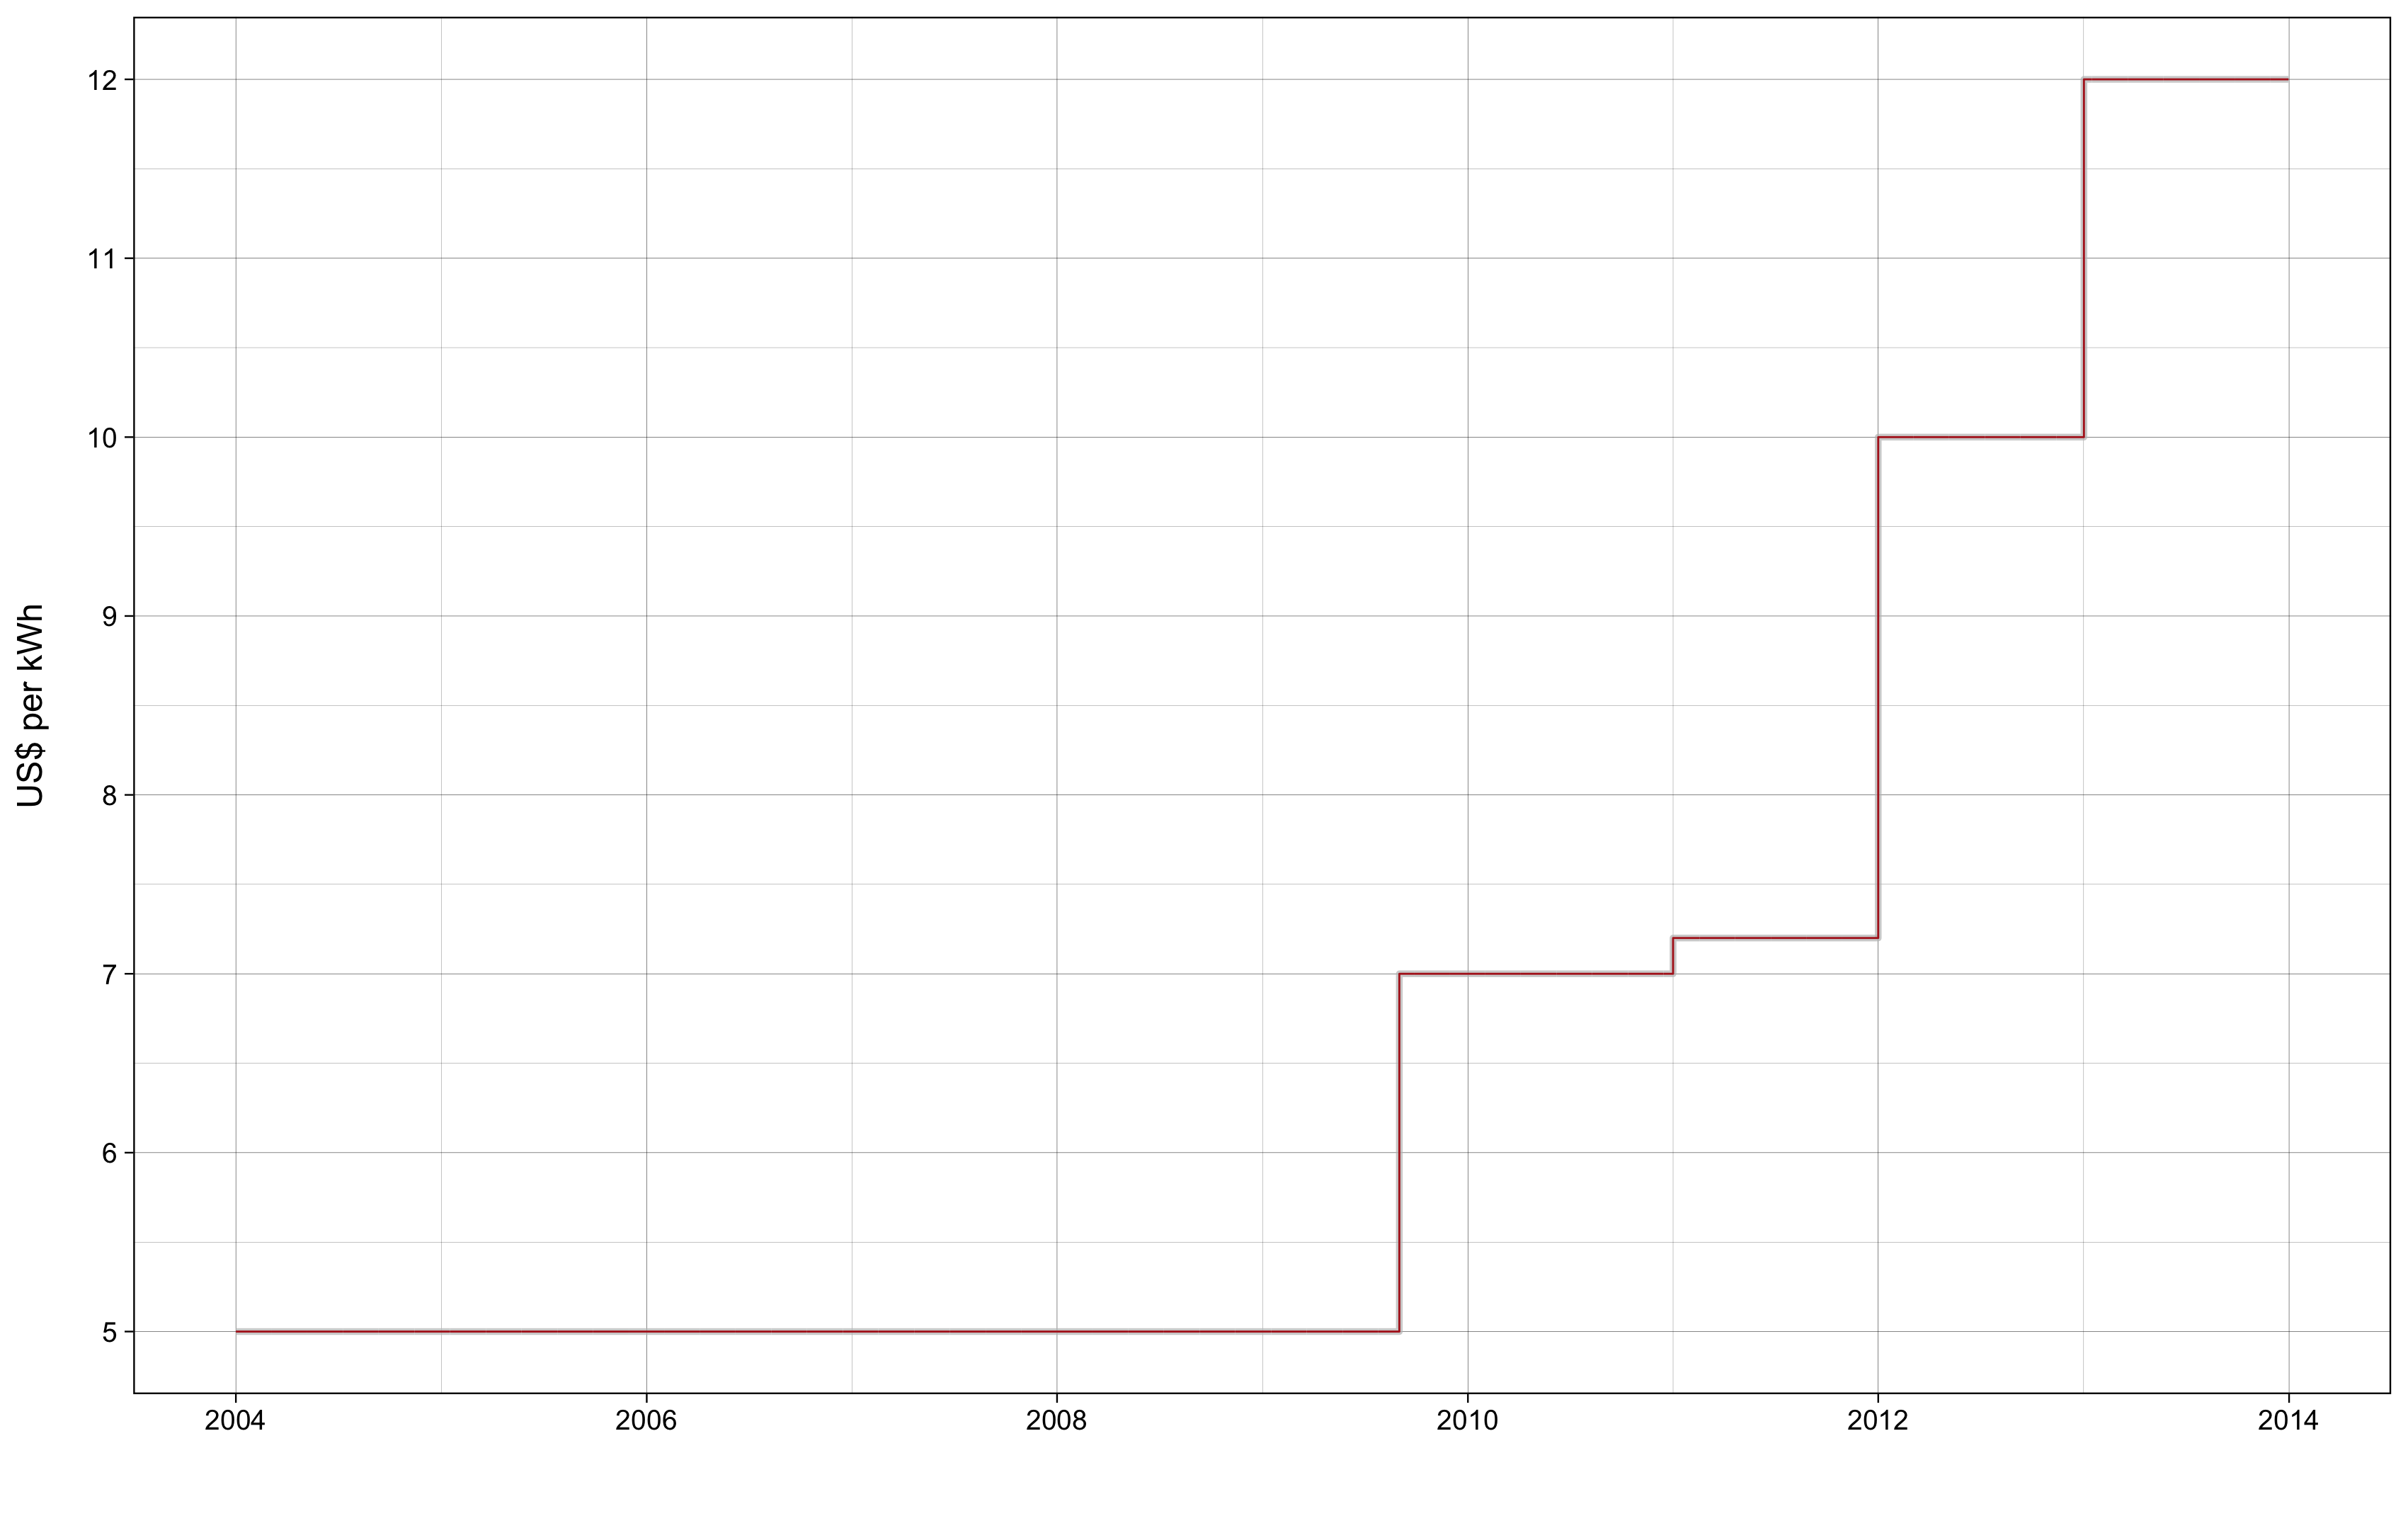
\includegraphics[scale = 0.133]{02_Chapter-1/00A_Figures/Figure_SMUD-Residential-Rates_Fixed-Charge.png}
        \caption{Fixed Charge of SMUD Residential Rates}
        \caption*{
            {\small
            \textit{Note}: 
            The figure shows how SMUD changed the monthly fixed charge over time. The same fixed charge applies to households that choose one of the three major residential rate plans (i.e., RSCH, RSEH, and RSGH).
        }}
        \label{Figure:SMUD-Residential-Rates_Fixed-Charge}
    \end{figure}
% }

\afterpage{
    \begin{figure}[t!]
        \centering
        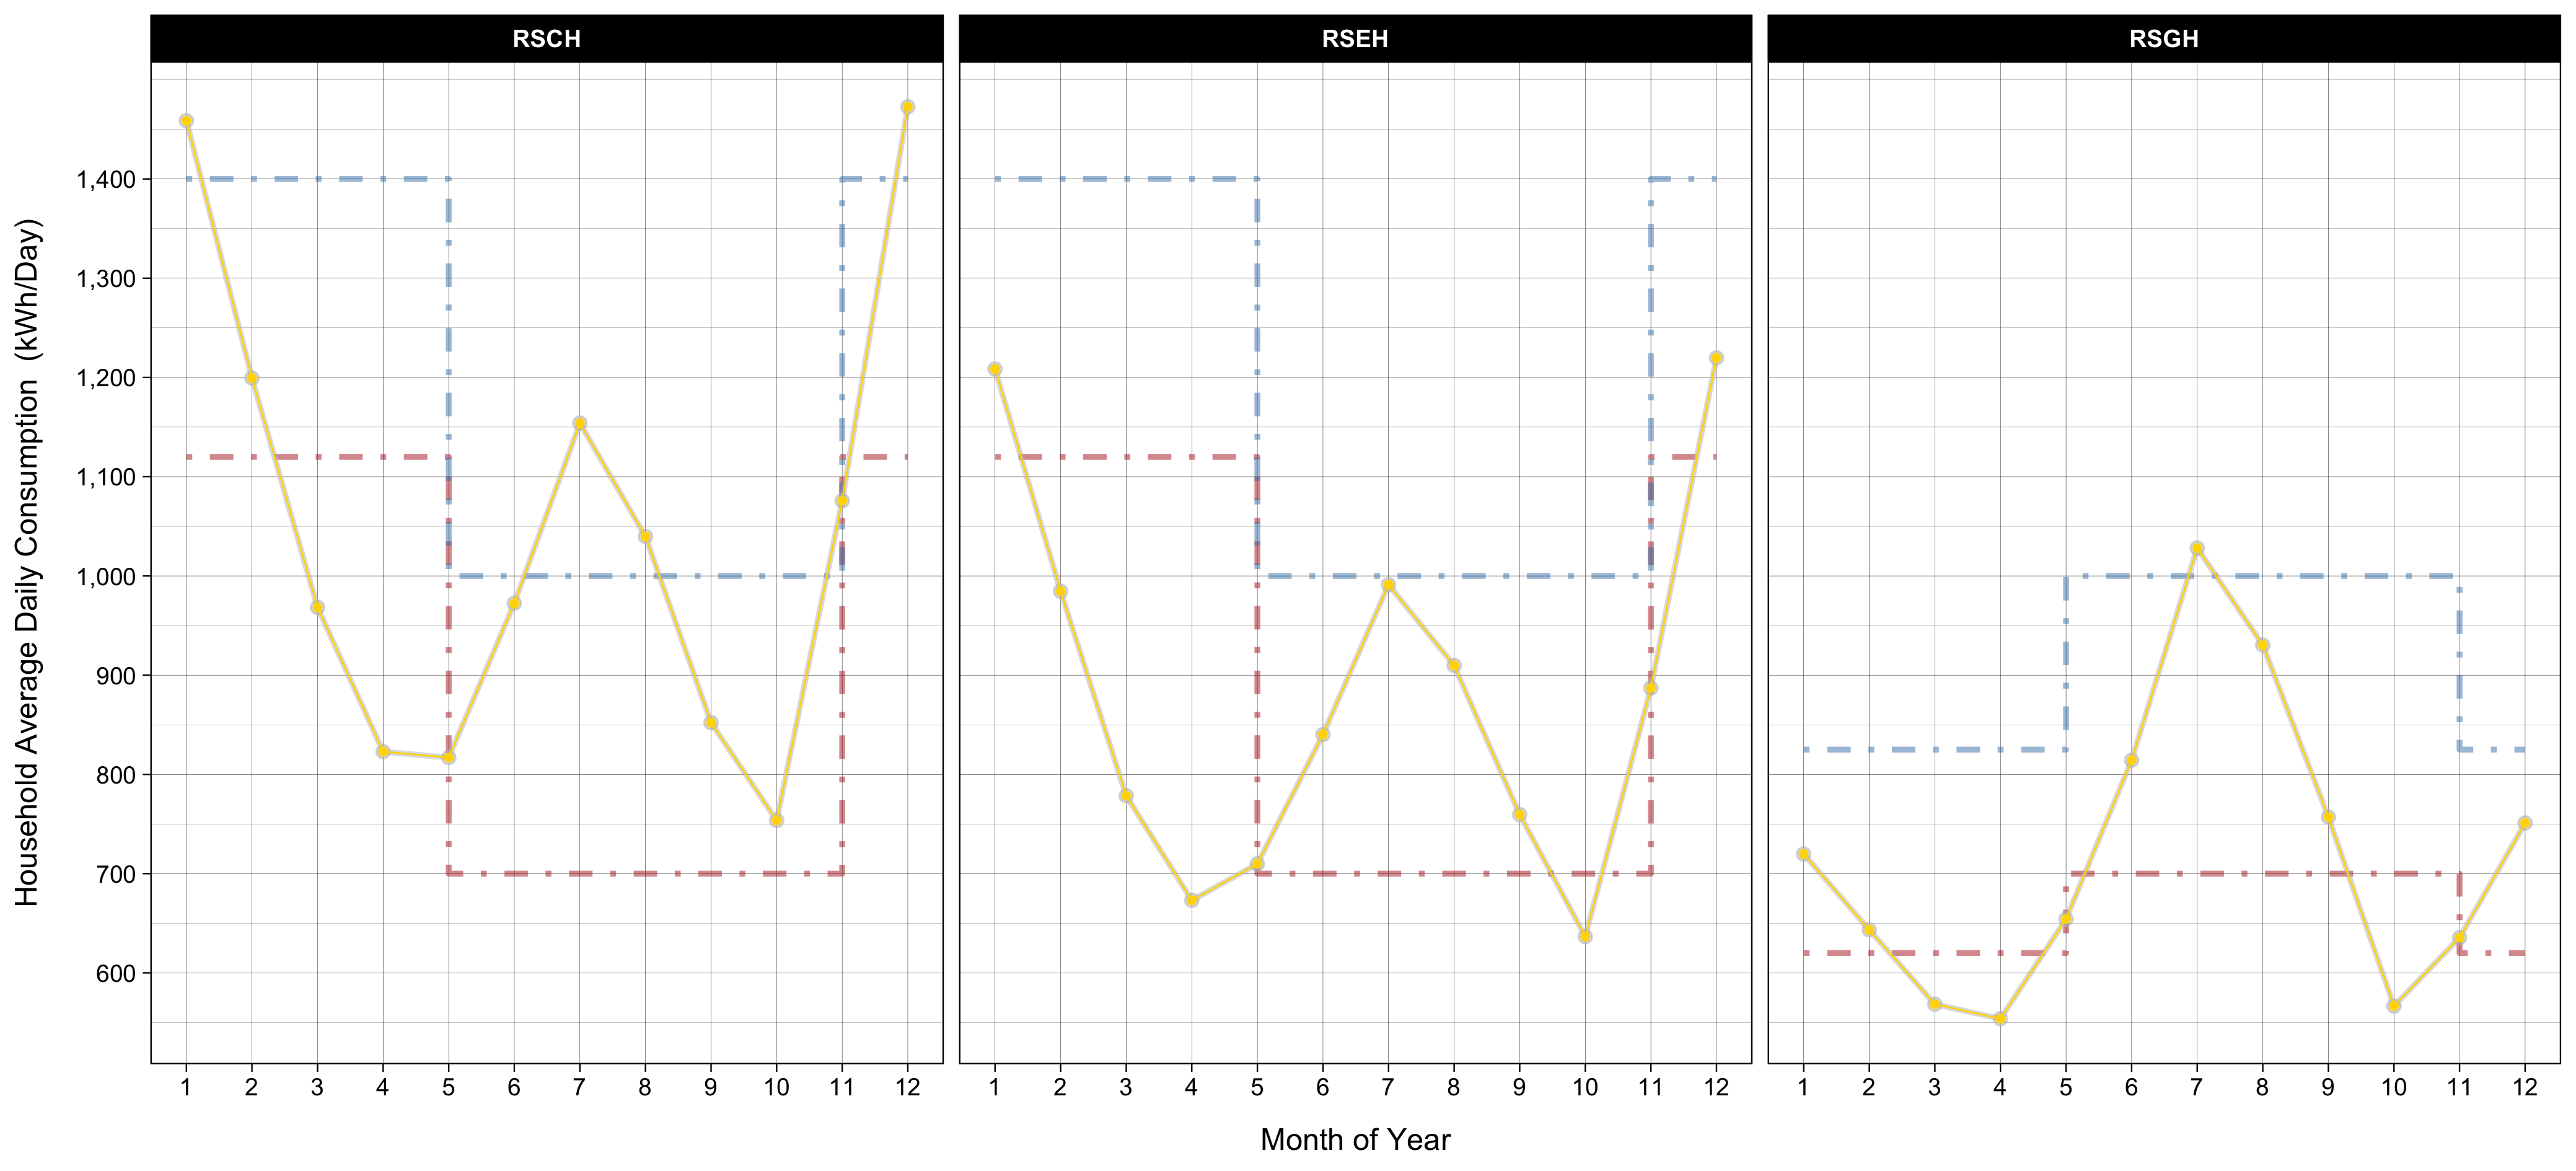
\includegraphics[scale = 0.105]{02_Chapter-1/00A_Figures/Figure_Household-Average-Daily-Consumption-by-Month.png}
        \caption{Household Average Daily Electricity Consumption by Month of Year}
        \caption*{
            {\small
            \textit{Note}: 
            This figure depicts, for each of SMUD residential rate plans, how households' average daily electricity consumption varied across months of the year. The red and blue dot-dash lines represent the lower and higher base usage quantities in each month of the year, respectively. The three rate plans show similar consumption and seasonal patterns. 
        }}
        \label{Figure:Household-Average-Daily-Electricity-Consumption-by-Month-of-Year}
    \end{figure}
}
\clearpage

% \afterpage{
    \begin{figure}[ht!]
        \centering
        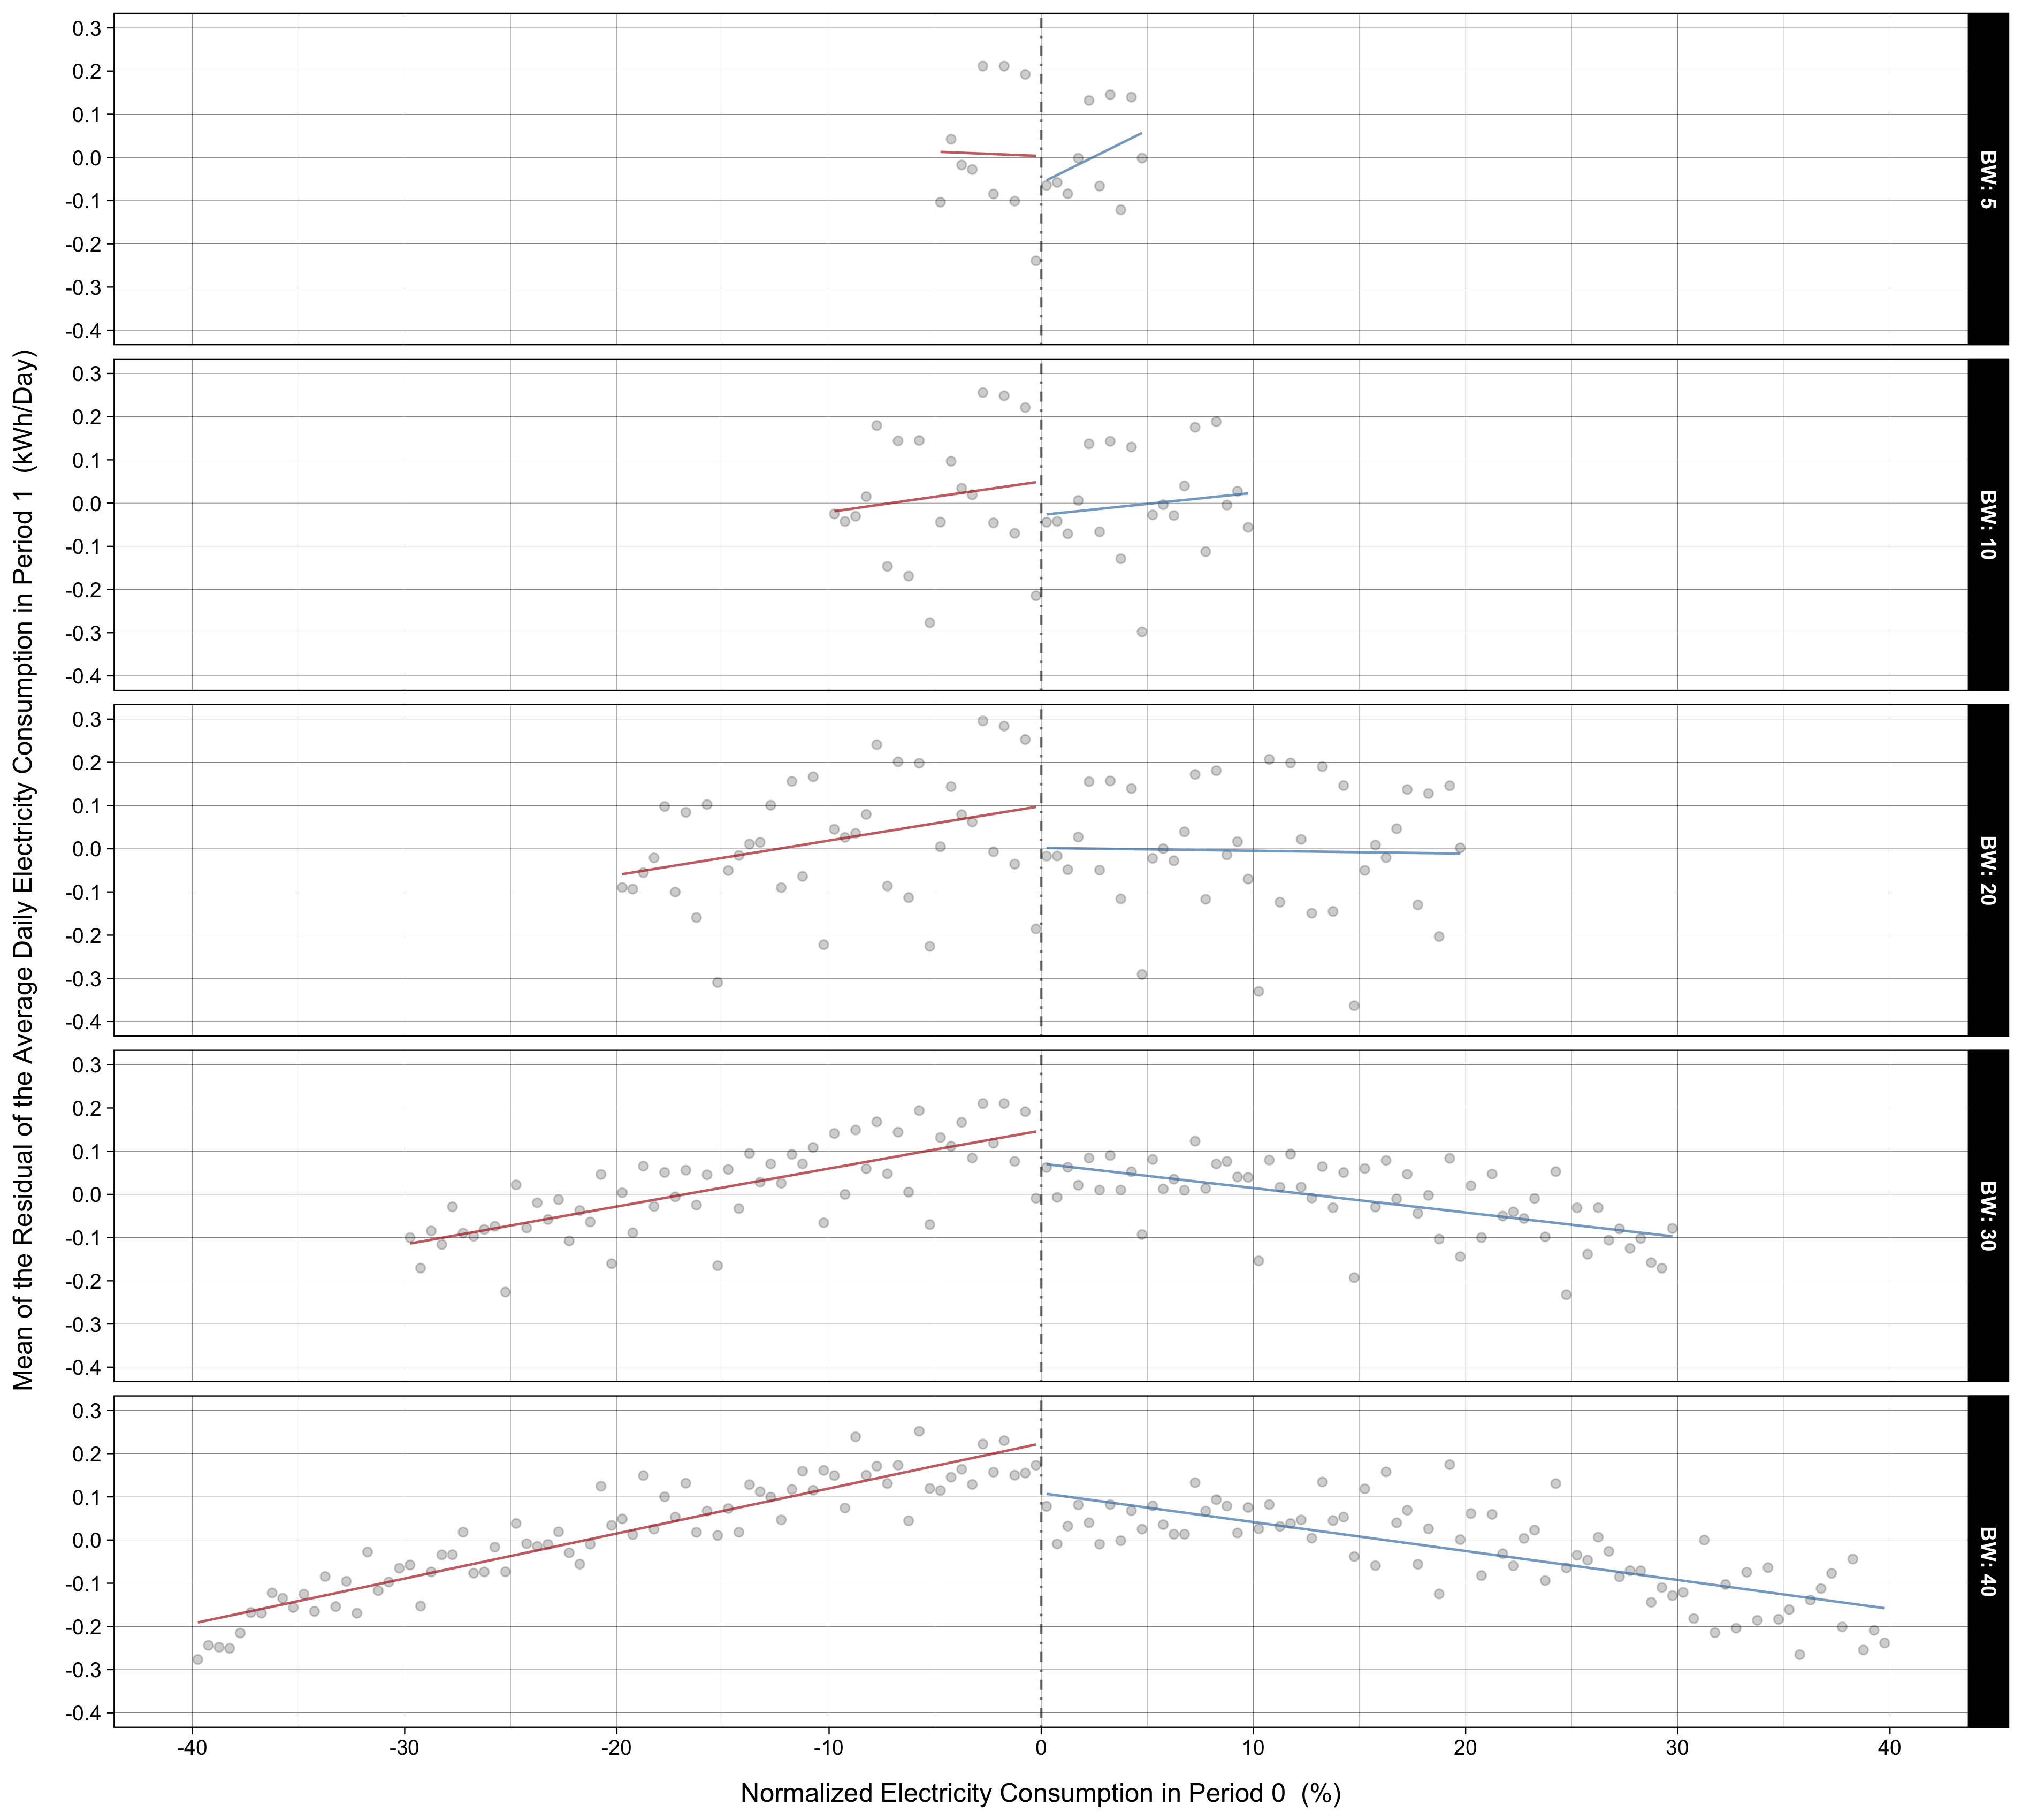
\includegraphics[scale = 0.120]{02_Chapter-1/00A_Figures/Figure_Residuals-of-the-Average-Daily-Electricity-Consumption-in-Period-0-over-NC0_From-BW5-to-BW40.png}
        \caption{The Impact of the Change in the Marginal Price due to Surpassing the Lower Base Usage Quantity}
        \caption*{
            {\small
            \textit{Note}: 
            In this figure, scatter dots correspond to the mean of residuals, computed by bins with a bandwidth of 0.5\%, from a regression of households' average daily electricity consumption in Period 1 on $\widebar{NC}_{0}$, HDDs and CDDs. As described, a linear model fits those scatter points well, even for a wide bandwidth. 
        }}
        \label{Figure:The-Impact-of-the-Change-in-the-MP-due-to-Surpassing-the-Lower-BUQ}
    \end{figure}
% }
\clearpage



% 2. Table(s)
\afterpage{
    \begin{table}[t!]
        \centering
        \caption{Robustness Checks: For Different Functional Forms, 3rd- and 4th-Order Polynomial Models}
        \label{Table:Robustness-Checks_Functional-Forms_3rd-and-4th-Order-Polynomial-Models}
        \vspace{0.3cm}
        \footnotesize
        \begin{adjustbox}{scale = 0.9}
            \begin{threeparttable}
                \begin{tabular}{@{\extracolsep{3pt}}lcccccccc}
                    \\[-5.5ex]
                    \hline \hline
                    \\[-3.0ex]
                     & \multicolumn{8}{c}{Dependent Variable} \\
                    \\[-3.0ex]
                    \cline{2-9}
                    \\[-3.0ex]
                     & \multicolumn{8}{c}{Average Daily Electricity Consumption  (kWh/Day)} \\
                    \\[-3.0ex]
                     & (1) & (2) & (3) & (4) & (5) & (6) & (7) & (8) \\
                    \\[-3.0ex]
                    \hline
                    \\[-2.0ex]
                    $\mathbb{1}$[Treatment] & 0.049 & $-$0.022 & $-$0.056$^{***}$ & $-$0.101$^{***}$ & 0.129$^{**}$ & 0.019 & $-$0.049$^{**}$ & $-$0.068$^{**}$ \\ 
                    & (0.042) & (0.025) & (0.017) & (0.028) & (0.051) & (0.037) & (0.021) & (0.027) \\ 
                    & & & & & & & & \\ 
                    NC0 & 0.143$^{***}$ & 0.211$^{***}$ & 0.215$^{***}$ & 0.225$^{***}$ & 0.111$^{**}$ & 0.207$^{***}$ & 0.213$^{***}$ & 0.217$^{***}$ \\ 
                    & (0.022) & (0.010) & (0.006) & (0.010) & (0.043) & (0.016) & (0.008) & (0.011) \\ 
                    & & & & & & & & \\ 
                    $\mathbb{1}$[Treatment] $\times$ NC0 & 0.056 & 0.005 & $-$0.007 & 0.0003 & $-$0.035 & $-$0.027 & $-$0.008 & $-$0.001 \\ 
                    & (0.035) & (0.013) & (0.005) & (0.005) & (0.079) & (0.021) & (0.008) & (0.010) \\ 
                    & & & & & & & & \\ 
                    NC0$^{2}$ & $-$0.020$^{***}$ & $-$0.002 & $-$0.0003 & $-$0.0001 & $-$0.035$^{**}$ & $-$0.003 & $-$0.001 & $-$0.001$^{*}$ \\ 
                    & (0.005) & (0.001) & (0.0002) & (0.0002) & (0.017) & (0.003) & (0.001) & (0.001) \\ 
                    & & & & & & & & \\ 
                    $\mathbb{1}$[Treatment] $\times$ NC0$^{2}$ & 0.022$^{***}$ & 0.001 & 0.0004 & $-$0.0004 & 0.092$^{***}$ & 0.010$^{**}$ & 0.001 & 0.001$^{**}$ \\ 
                    & (0.008) & (0.001) & (0.0003) & (0.0003) & (0.024) & (0.005) & (0.001) & (0.001) \\ 
                    & & & & & & & & \\ 
                    NC0$^{3}$ & $-$0.001$^{***}$ & $-$0.00005 & $-$0.00000 & 0.00000 & $-$0.004 & $-$0.0001 & $-$0.00002 & $-$0.00003$^{*}$ \\ 
                    & (0.0003) & (0.00003) & (0.00001) & (0.00000) & (0.002) & (0.0002) & (0.00004) & (0.00002) \\ 
                    & & & & & & & & \\ 
                    $\mathbb{1}$[Treatment] $\times$ NC0$^{3}$ & 0.001$^{**}$ & 0.0001 & $-$0.00000 & 0.00000 & $-$0.005 & $-$0.0005$^{*}$ & $-$0.00001 & $-$0.00000 \\ 
                    & (0.001) & (0.00005) & (0.00001) & (0.00001) & (0.005) & (0.0003) & (0.0001) & (0.00004) \\ 
                    & & & & & & & & \\ 
                    NC0$^{4}$ &  &  &  &  & $-$0.0001 & $-$0.00000 & $-$0.00000 & $-$0.00000$^{*}$ \\ 
                    &  &  &  &  & (0.0001) & (0.00000) & (0.00000) & (0.00000) \\ 
                    & & & & & & & & \\ 
                    $\mathbb{1}$[Treatment] $\times$ NC0$^{4}$ &  &  &  &  & 0.001$^{***}$ & 0.00002$^{*}$ & 0.00000 & 0.00000$^{**}$ \\ 
                    &  &  &  &  & (0.0002) & (0.00001) & (0.00000) & (0.00000) \\ 
                    & & & & & & & & \\ 
                    Average Daily CDDs & 1.146$^{***}$ & 1.146$^{***}$ & 1.135$^{***}$ & 1.133$^{***}$ & 1.146$^{***}$ & 1.146$^{***}$ & 1.135$^{***}$ & 1.133$^{***}$ \\ 
                    & (0.106) & (0.105) & (0.109) & (0.129) & (0.106) & (0.105) & (0.109) & (0.129) \\ 
                    & & & & & & & & \\ 
                    Average Daily HDDs & 0.428$^{***}$ & 0.431$^{***}$ & 0.375$^{***}$ & 0.742$^{***}$ & 0.428$^{***}$ & 0.431$^{***}$ & 0.375$^{***}$ & 0.742$^{***}$ \\ 
                    & (0.106) & (0.104) & (0.128) & (0.202) & (0.106) & (0.104) & (0.128) & (0.202) \\ 
                    & & & & & & & & \\
                    \hline
                    \\[-2.0ex]
                    Bandwidth & 10\% & 20\% & 30\% & 40\% & 10\% & 20\% & 30\% & 40\% \\ 
                    FEs: Billing Year-by-Month & Yes & Yes & Yes & Yes & Yes & Yes & Yes & Yes \\ 
                    Observations & 2,378,864 & 4,702,081 & 6,276,579 & 3,904,120 & 2,378,864 & 4,702,081 & 6,276,579 & 3,904,120 \\ 
                    Adjusted R$^{2}$ & 0.293 & 0.334 & 0.536 & 0.592 & 0.293 & 0.334 & 0.536 & 0.592 \\
                    \\[-2.0ex]
                    \hline \hline
                    \\[-4.5ex]
                \end{tabular}
                \begin{tablenotes}[flushleft]
                    \footnotesize
                    \item \textit{Note}: * $p < 0.1$, ** $p < 0.05$, and *** $p < 0.01$.
                \end{tablenotes}
            \end{threeparttable}
        \end{adjustbox}
        
    \end{table}
}

\clearpage

\afterpage{
    \begin{table}[t!]
        \centering
        \caption{Robustness Checks: For Different Bandwidths, Without FEs}
        \label{Table:Robustness-Checks_BWs_Without-FEs}
        \vspace{0.3cm}
        \footnotesize
        \begin{adjustbox}{scale = 0.76}
            \begin{threeparttable}
                \begin{tabular}{@{\extracolsep{5pt}}lcccccccc}
                    \\[-5.5ex]
                    \hline \hline
                    \\[-3.0ex]
                     & \multicolumn{8}{c}{Dependent Variable} \\
                    \\[-3.0ex]
                    \cline{2-9}
                    \\[-3.0ex]
                     & \multicolumn{8}{c}{Average Daily Electricity Consumption  (kWh/Day)} \\
                    \\[-3.0ex]
                     & (1) & (2) & (3) & (4) & (5) & (6) & (7) & (8) \\
                    \\[-3.0ex]
                    \hline
                    \\[-2.0ex]
                    $\mathbb{1}$[Treatment] & $-$0.014 & $-$0.054$^{*}$ & $-$0.053$^{*}$ & $-$0.084$^{***}$ & $-$0.076$^{***}$ & $-$0.072$^{**}$ & $-$0.097$^{*}$ & $-$0.118$^{*}$ \\ 
                    & (0.032) & (0.030) & (0.028) & (0.028) & (0.029) & (0.031) & (0.056) & (0.064) \\ 
                    & & & & & & & & \\ 
                    NC0 & 0.169$^{***}$ & 0.197$^{***}$ & 0.202$^{***}$ & 0.204$^{***}$ & 0.204$^{***}$ & 0.199$^{***}$ & 0.214$^{***}$ & 0.211$^{***}$ \\ 
                    & (0.010) & (0.007) & (0.006) & (0.006) & (0.006) & (0.006) & (0.009) & (0.009) \\ 
                    & & & & & & & & \\ 
                    $\mathbb{1}$[Treatment] $\times$ NC0 & 0.038$^{***}$ & 0.001 & $-$0.010$^{***}$ & $-$0.008$^{***}$ & $-$0.009$^{***}$ & $-$0.014$^{***}$ & $-$0.018$^{***}$ & $-$0.017$^{***}$ \\ 
                    & (0.012) & (0.004) & (0.003) & (0.003) & (0.003) & (0.003) & (0.004) & (0.005) \\ 
                    & & & & & & & & \\ 
                    Average Daily CDDs & 0.749$^{***}$ & 0.753$^{***}$ & 0.755$^{***}$ & 0.757$^{***}$ & 0.758$^{***}$ & 0.767$^{***}$ & 0.932$^{***}$ & 1.143$^{***}$ \\ 
                    & (0.122) & (0.121) & (0.120) & (0.119) & (0.118) & (0.114) & (0.124) & (0.124) \\ 
                    & & & & & & & & \\ 
                    Average Daily HDDs & 0.280$^{***}$ & 0.281$^{***}$ & 0.282$^{***}$ & 0.284$^{***}$ & 0.286$^{***}$ & 0.152$^{**}$ & 0.637$^{***}$ & 1.033$^{***}$ \\ 
                    & (0.079) & (0.078) & (0.078) & (0.077) & (0.077) & (0.066) & (0.101) & (0.131) \\ 
                    & & & & & & & & \\ 
                    (Constant) & 19.947$^{***}$ & 19.973$^{***}$ & 19.972$^{***}$ & 19.965$^{***}$ & 19.937$^{***}$ & 19.720$^{***}$ & 17.769$^{***}$ & 15.117$^{***}$ \\ 
                    & (0.948) & (0.941) & (0.937) & (0.932) & (0.926) & (0.829) & (1.082) & (1.159) \\ 
                    & & & & & & & & \\
                    \hline
                    \\[-2.0ex]
                    Bandwidth & 5\% & 10\% & 15\% & 20\% & 25\% & 30\% & 35\% & 40\% \\ 
                    FEs: Billing Year-by-Month & No & No & No & No & No & No & No & No \\ 
                    Observations & 1,186,630 & 2,378,864 & 3,566,318 & 4,702,081 & 5,816,854 & 6,276,579 & 4,093,259 & 3,904,120 \\ 
                    Adjusted R$^{2}$ & 0.105 & 0.120 & 0.144 & 0.175 & 0.210 & 0.349 & 0.394 & 0.468 \\
                    \\[-2.0ex]
                    \hline \hline
                    \\[-4.5ex]
                \end{tabular}
                \begin{tablenotes}[flushleft]
                    \footnotesize
                    \item \textit{Note}: Contrary to Table \ref{Table:Robustness-Checks_BWs}, this table reports the results of robustness checks for a range of bandwidths using the regression in the specification (5) in Table \ref{Table:RD-Results}. Standard errors in parentheses are clustered at the household and billing year-by-month levels to allow correlations across households in a given month; * $p < 0.1$, ** $p < 0.05$, and *** $p < 0.01$.
                \end{tablenotes}
            \end{threeparttable}
        \end{adjustbox}
    \end{table}
}

\clearpage

\afterpage{
    \begin{table}[t!]
        \centering
        \caption{Robustness Checks: For Different Bandwidths, Only RSGH Rate Code}
        \label{Table:Robustness-Checks_BWs_RSGH}
        \vspace{0.3cm}
        \small
        \begin{adjustbox}{scale = 0.72}
            \begin{threeparttable}
                \begin{tabular}{@{\extracolsep{5pt}}lcccccccc}
                    \\[-5.5ex]
                    \hline \hline
                    \\[-3.0ex]
                    & \multicolumn{8}{c}{Dependent Variable} \\
                    \\[-3.0ex]
                    \cline{2-9}
                    \\[-3.0ex]
                    & \multicolumn{8}{c}{Average Daily Electricity Consumption  (kWh/Day)} \\
                    \\[-3.0ex]
                    & (1) & (2) & (3) & (4) & (5) & (6) & (7) & (8) \\
                    \\[-3.0ex]
                    \hline
                    \\[-2.0ex]
                    $\mathbb{1}$[Treatment] & $-$0.055$^{***}$ & $-$0.060$^{***}$ & $-$0.055$^{***}$ & $-$0.065$^{***}$ & $-$0.064$^{***}$ & $-$0.058$^{***}$ & $-$0.068$^{***}$ & $-$0.080$^{***}$ \\ 
                    & (0.020) & (0.016) & (0.015) & (0.014) & (0.013) & (0.013) & (0.021) & (0.024) \\ 
                    & & & & & & & & \\ 
                    NC0 & 0.211$^{***}$ & 0.215$^{***}$ & 0.215$^{***}$ & 0.216$^{***}$ & 0.216$^{***}$ & 0.217$^{***}$ & 0.234$^{***}$ & 0.229$^{***}$ \\ 
                    & (0.008) & (0.006) & (0.005) & (0.005) & (0.005) & (0.006) & (0.008) & (0.010) \\ 
                    & & & & & & & & \\ 
                    $\mathbb{1}$[Treatment] $\times$ NC0 & $-$0.005 & $-$0.010$^{***}$ & $-$0.013$^{***}$ & $-$0.012$^{***}$ & $-$0.014$^{***}$ & $-$0.016$^{***}$ & $-$0.021$^{***}$ & $-$0.020$^{***}$ \\ 
                    & (0.006) & (0.003) & (0.002) & (0.001) & (0.002) & (0.002) & (0.003) & (0.004) \\ 
                    & & & & & & & & \\ 
                    Average Daily CDDs & 1.170$^{***}$ & 1.172$^{***}$ & 1.174$^{***}$ & 1.174$^{***}$ & 1.172$^{***}$ & 1.171$^{***}$ & 1.162$^{***}$ & 1.190$^{***}$ \\ 
                    & (0.106) & (0.108) & (0.108) & (0.107) & (0.107) & (0.106) & (0.114) & (0.126) \\ 
                    & & & & & & & & \\ 
                    Average Daily HDDs & 0.224$^{**}$ & 0.227$^{**}$ & 0.227$^{**}$ & 0.228$^{**}$ & 0.228$^{**}$ & 0.229$^{**}$ & 0.547$^{***}$ & 0.708$^{***}$ \\ 
                    & (0.090) & (0.090) & (0.090) & (0.089) & (0.088) & (0.087) & (0.133) & (0.186) \\ 
                    & & & & & & & & \\
                    \hline
                    \\[-2.0ex]
                    Rate Code & RSGH & RSGH & RSGH & RSGH & RSGH & RSGH & RSGH & RSGH \\ 
                    Bandwidth & 5\% & 10\% & 15\% & 20\% & 25\% & 30\% & 35\% & 40\% \\ 
                    FEs: Billing Year-by-Month & Yes & Yes & Yes & Yes & Yes & Yes & Yes & Yes \\ 
                    Observations & 967,546 & 1,941,332 & 2,909,164 & 3,832,683 & 4,738,070 & 5,604,830 & 3,396,312 & 3,191,411 \\ 
                    Adjusted R$^{2}$ & 0.475 & 0.486 & 0.503 & 0.524 & 0.547 & 0.571 & 0.576 & 0.613 \\
                    \\[-2.0ex]
                    \hline \hline
                    \\[-4.5ex]
                \end{tabular}
                \begin{tablenotes}[flushleft]
                    \footnotesize
                    \item \textit{Note}: This table shows the results of regressions with observations only for households selecting the RSGH rate plan. Standard errors in parentheses are clustered at the household and billing year-by-month levels to allow correlations across households in a given month; * $p < 0.1$, ** $p < 0.05$, and *** $p < 0.01$.
                \end{tablenotes}
            \end{threeparttable}
        \end{adjustbox}
    \end{table}
}

\clearpage



\clearpage
\section{For Chapter 2}
\subsection{Additional Figure(s) and Table(s)}
% 1. Figure(s)
%\afterpage{
    \begin{figure}[!ht]
        \centering
        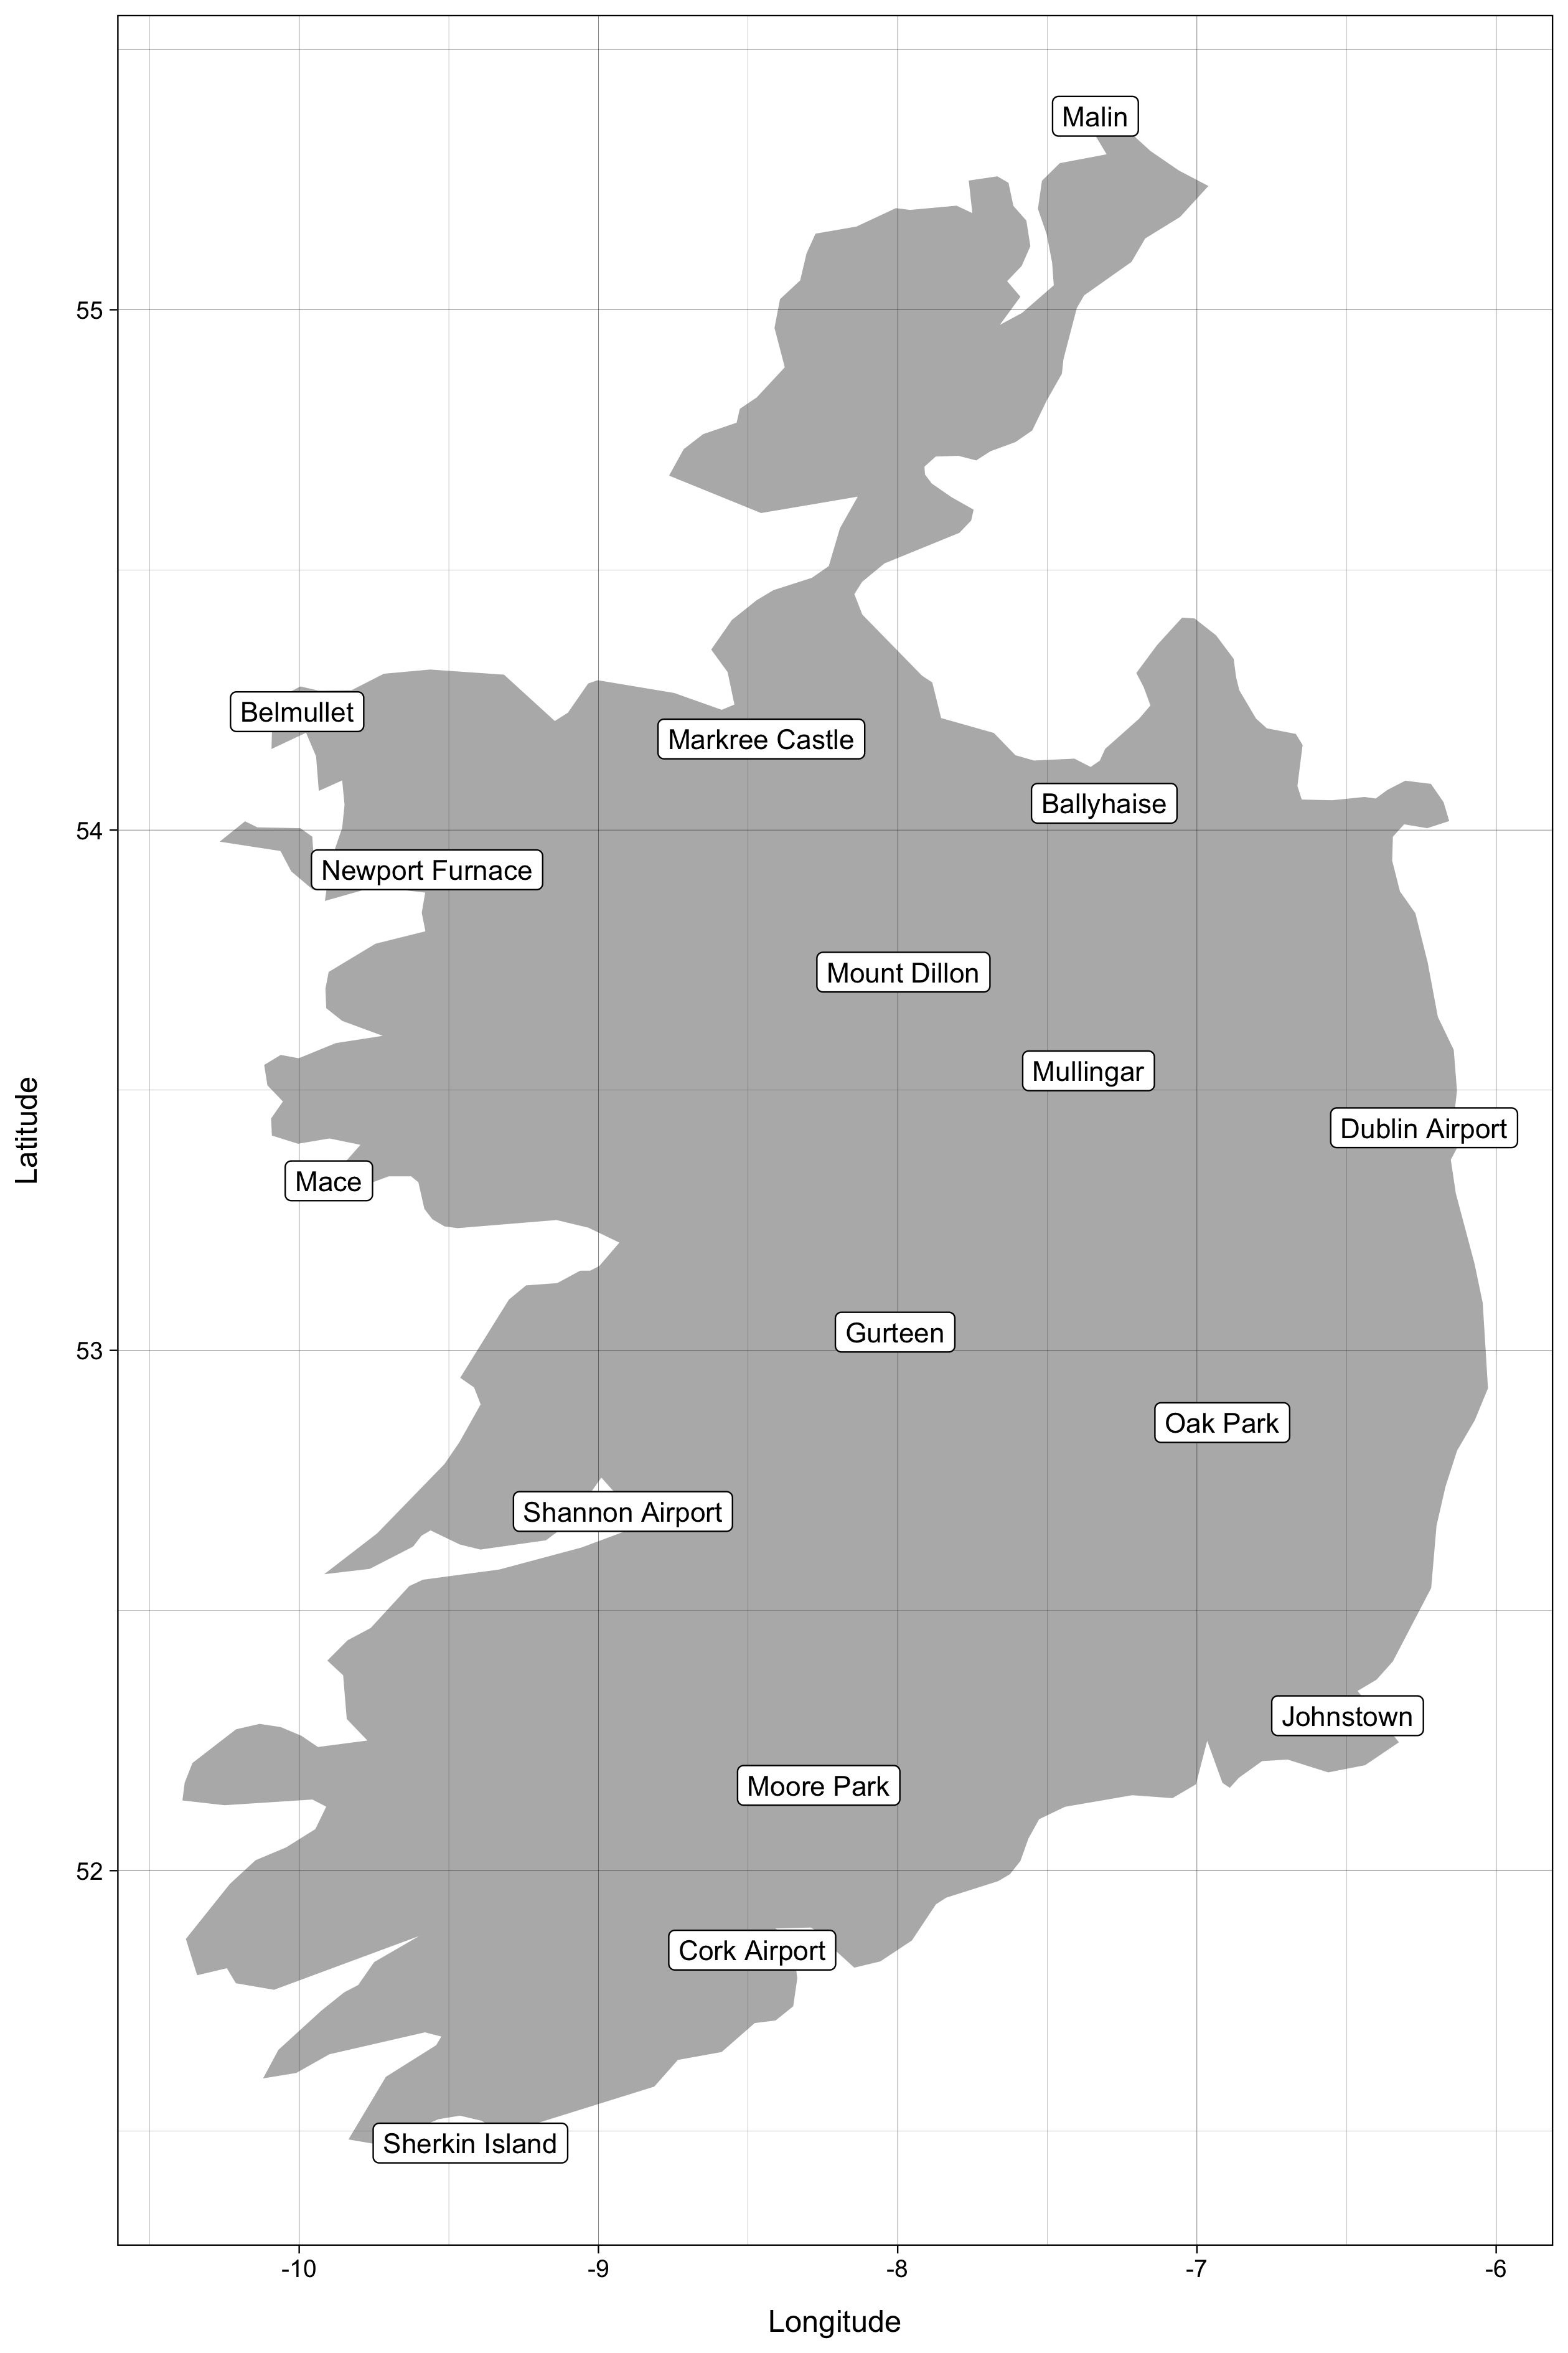
\includegraphics[scale = 0.13]{03_Chapter-2/00A_Figures/Figure_Location-of-Weather-Stations.png}
        \caption{Weather Stations from which Historical Weather Data have been collected}
        \caption*{
            {\small
            \textit{Note}: This figure demonstrates the location of each weather station listed in Table \ref{Table:Correlations-in-Average-Daily-Temperatures-among-Weather-Stations}. As is evident from the map, the weather stations are distributed throughout Ireland.
        }}
        \label{Figure:Weather-Stations}
    \end{figure}
%}
\clearpage



% 2. Table(s)
\afterpage{
    \begin{table}[t!]
        \centering
        \caption{Correlations in Average Daily Temperatures between Weather Stations}
        \label{Table:Correlations-in-Average-Daily-Temperatures-among-Weather-Stations}
        \vspace{0.2cm}
        \begin{adjustbox}{scale = 1.0}
            \begin{tabular}{
                >{\raggedright}m{4.8cm} |
                >{\centering}m{5.5cm} 
                >{\centering\arraybackslash}m{5.5cm}
            }
                \hline \hline
                \multicolumn{1}{c|}{Stations} & \multicolumn{2}{c}{Correlation Coefficients} \\
                \cline{2-3}
                \multicolumn{1}{c|}{}  & \multicolumn{1}{c}{For Sample Period} & \multicolumn{1}{c}{For Experiment Period} \\
                \hline
                Ballyhaise & 0.98291 & 0.98244 \\
                Belmullet & 0.96089 & 0.96361 \\
                Cork Airport & 0.97121 & 0.97130 \\
                Gurteen & 0.98389 & 0.98307 \\
                Johnstown & 0.98189 & 0.97958 \\
                Mace & 0.95870 & 0.95921 \\
                Malin & 0.95632 & 0.95705 \\
                Markree Castle & 0.97194 & 0.97179 \\
                Moore Park & 0.98057 & 0.97798 \\
                Mount Dillon & 0.97945 & 0.97782 \\
                Mullingar & 0.98876 & 0.98654 \\
                Newport Furnace & 0.97015 & 0.97211 \\
                Oak Park & 0.99074 & 0.98925 \\
                Shannon Airport & 0.97696 & 0.97582 \\
                Sherkin Island & 0.95342 & 0.95411 \\
                \hline \hline
            \end{tabular}
        \end{adjustbox}
        \begin{tablenotes}[flushleft]
            \small
            \textit{Note}: For each weather station, historical weather data from the weather station at Dublin airport is utilized to compute the two correlation coefficients. I do not provide the $p$-value of each correlation coefficient because it is arbitrarly small in magnitude. And the experiment period is the period between July 2009 to December 2010, while the sample period is the second half of 2009 and 2010. 
        \end{tablenotes}
    \end{table}
}


\afterpage{
    \begin{landscape} 
    \begin{table}[t!]
        \centering
        \caption{Hourly Average Treatment Effects in and near the Peak Rate Period}
        \label{Table:Hourly-Average-Treatment-Effects-in-and-near-the-Peak-Rate-Period_For-Appendix}
        \vspace{0.3cm}
        \small
        \begin{adjustbox}{scale = 0.7}
            \begin{threeparttable}
                \begin{tabular}{@{\extracolsep{1pt}}lcccccccccccc}
                    \\[-4.0ex]
                    \hline \hline
                    \\[-3.0ex]
%                    & \multicolumn{15}{c}{Dependent Variable} \\
%                    \\[-3.0ex]
%                    \cline{2-16}
%                    \\[-3.0ex]
                    & \multicolumn{12}{c}{Hourly Electricity Consumption  (kWh/Hour)} \\
                    \\[-3.0ex]
                    & (1) & (2) & (3) & (4) & (5) & (6) & (7) & (8) & (9) & (10) & (11) & (12) \\
                    \\[-3.0ex]
                    \hline
                    \\[-2.0ex]
                    $\mathbb{1}$[Treatment \& Post] & $-$0.048$^{***}$ & $-$0.053$^{*}$ & $-$0.002 & $-$0.049 & $-$0.125$^{***}$ & $-$0.161$^{***}$ & $-$0.119$^{***}$ & $-$0.249$^{***}$ & $-$0.082$^{***}$ & $-$0.055$^{*}$ & $-$0.015 & $-$0.113$^{**}$ \\
                    & (0.016) & (0.027) & (0.017) & (0.031) & (0.020) & (0.036) & (0.022) & (0.044) & (0.020) & (0.030) & (0.021) & (0.048) \\
                    & & & & & & & & & & & & \\
                    \hline
                    \\[-2.0ex]
                    Description of Period & Pre-Peak & Pre-Peak & Pre-Peak & Pre-Peak & Peak & Peak & Peak & Peak & Post-Peak & Post-Peak & Post-Peak & Post-Peak \\
                    Period of Hours & 15 to 16 & 15 to 16 & 15 to 16 & 15 to 16 & 17 to 18 & 17 to 18 & 17 to 18 & 17 to 18 & 19 to 20 & 19 to 20 & 19 to 20 & 19 to 20 \\
                    Tariff Group & A & B & C & D & A & B & C & D & A & B & C & D \\
                    Price Change in the Peak Rate Period & +6 & +12 & +18 & +24 & +6 & +12 & +18 & +24 & +6 & +12 & +18 & +24 \\
                    FEs: Household by Half-Hourly Time Window & Yes & Yes & Yes & Yes & Yes & Yes & Yes & Yes & Yes & Yes & Yes & Yes \\
                    FEs: Day of Week by Half-Hourly Time Window & Yes & Yes & Yes & Yes & Yes & Yes & Yes & Yes & Yes & Yes & Yes & Yes \\
                    FEs: Month of Year & Yes & Yes & Yes & Yes & Yes & Yes & Yes & Yes & Yes & Yes & Yes & Yes \\
                    Observations & 506,540 & 326,800 & 511,700 & 331,960 & 506,540 & 326,800 & 511,700 & 331,960 & 506,540 & 326,800 & 511,700 & 331,960 \\
                    Adjusted R$^{2}$ & 0.312 & 0.330 & 0.320 & 0.327 & 0.384 & 0.397 & 0.383 & 0.367 & 0.371 & 0.389 & 0.376 & 0.361 \\
                    \\[-2.0ex]
                    \hline \hline
                    \\[-4.5ex]
                \end{tabular}
                \begin{tablenotes}[flushleft]
                    \footnotesize
                    \item \textit{Note}: * $p < 0.1$, ** $p < 0.05$, and *** $p < 0.01$.
                \end{tablenotes}
            \end{threeparttable}
        \end{adjustbox}
    \end{table} 
    \end{landscape}
}

\clearpage

%\afterpage{
    \begin{ThreePartTable}
        \centering
        \scriptsize
        \vspace{0.5cm}
        \renewcommand\TPTminimum{\textwidth}
        
        \begin{TableNotes}[flushleft]
            \scriptsize
%            \item
            \item \textit{Note}: * $p < 0.1$, ** $p < 0.05$, and *** $p < 0.01$.
        \end{TableNotes}
        
        \begin{landscape}
        \begin{longtable}{@{\extracolsep{1.5pt}}lcccccccc}
            \caption{Breakdown of Hourly Average Treatment Effects}
            \label{Table:Breakdown-of-Hourly-ATEs_For-Appendix} \\

            \\[-4.0ex]
            \hline \hline
            \\[-3.0ex]
            & \multicolumn{8}{c}{Hourly Electricity Consumption  (kWh/Hour)} \\
            \\[-3.0ex]
            & (1) & (2) & (3) & (4) & (5) & (6) & (7) & (8) \\
            \\[-3.0ex]
            \hline
            \\[-2.0ex]
            \endfirsthead

            \multicolumn{9}{c}{{\bfseries \tablename \ \thetable{} -- continued from previous page}} \\

            \hline \hline
            \\[-3.0ex]
            & \multicolumn{8}{c}{Hourly Electricity Consumption  (kWh/Hour)} \\
            \\[-3.0ex]
            & (1) & (2) & (3) & (4) & (5) & (6) & (7) & (8) \\
            \\[-3.0ex]
            \hline
            \\[-2.0ex]
            \endhead

            \multicolumn{9}{r}{{\footnotesize{\textit{(Continued on next page...)}}}} \\
            \endfoot
            \insertTableNotes
            \endlastfoot

            HDDs & 0.016$^{***}$ & 0.016$^{***}$ & 0.016$^{***}$ & 0.015$^{***}$ & 0.047$^{***}$ & 0.047$^{***}$ & 0.047$^{***}$ & 0.047$^{***}$ \\
            & (0.004) & (0.004) & (0.004) & (0.004) & (0.004) & (0.004) & (0.004) & (0.004) \\
            & & & & & & & & \\
            HDDs$^{*}$ & 0.010 & 0.009 & 0.009 & 0.010 & $-$0.018$^{***}$ & $-$0.018$^{***}$ & $-$0.018$^{***}$ & $-$0.018$^{***}$ \\
            & (0.007) & (0.007) & (0.007) & (0.007) & (0.007) & (0.007) & (0.007) & (0.007) \\
            & & & & & & & & \\
            $\mathbb{1}$[Treatment] & 0.009 & 0.106 & $-$0.014 & 0.174$^{**}$ & 0.057 & 0.189$^{**}$ & $-$0.017 & 0.150$^{**}$ \\
            & (0.050) & (0.071) & (0.049) & (0.072) & (0.055) & (0.083) & (0.052) & (0.072) \\
            & & & & & & & & \\
            $\mathbb{1}$[Treatment] $\times$ HDDs & 0.001 & 0.004 & 0.001 & 0.0003 & 0.009$^{**}$ & 0.008 & 0.008$^{**}$ & 0.011 \\
            & (0.003) & (0.005) & (0.003) & (0.004) & (0.004) & (0.007) & (0.004) & (0.007) \\
            & & & & & & & & \\
            $\mathbb{1}$[Treatment] $\times$ HDDs$^{*}$ & $-$0.0001 & $-$0.012$^{*}$ & 0.0004 & 0.002 & $-$0.012$^{***}$ & $-$0.016$^{**}$ & $-$0.013$^{***}$ & $-$0.008 \\
            & (0.004) & (0.006) & (0.003) & (0.005) & (0.004) & (0.008) & (0.004) & (0.007) \\
            & & & & & & & & \\
            $\mathbb{1}$[Post] & 0.014 & 0.015 & 0.014 & 0.011 & 0.048 & 0.049 & 0.047 & 0.047 \\
            & (0.022) & (0.022) & (0.022) & (0.023) & (0.040) & (0.040) & (0.040) & (0.040) \\
            & & & & & & & & \\
            $\mathbb{1}$[Post] $\times$ HDDs & $-$0.007 & $-$0.007 & $-$0.007 & $-$0.006 & $-$0.015$^{**}$ & $-$0.015$^{**}$ & $-$0.015$^{**}$ & $-$0.015$^{**}$ \\
            & (0.005) & (0.005) & (0.005) & (0.005) & (0.006) & (0.006) & (0.006) & (0.006) \\
            & & & & & & & & \\
            $\mathbb{1}$[Post] $\times$ HDDs$^{*}$ & 0.002 & 0.002 & 0.002 & 0.001 & 0.006 & 0.007 & 0.006 & 0.006 \\
            & (0.008) & (0.008) & (0.008) & (0.008) & (0.009) & (0.009) & (0.009) & (0.009) \\
            & & & & & & & & \\
            & & & & & & & & \\
            & & & & & & & & \\
            $\mathbb{1}$[Treatment \& Post] & $-$0.038 & $-$0.039 & 0.020 & $-$0.039 & $-$0.040 & $-$0.050 & 0.006 & $-$0.025 \\
            & (0.023) & (0.030) & (0.026) & (0.038) & (0.029) & (0.037) & (0.027) & (0.040) \\
            & & & & & & & & \\
            $\mathbb{1}$[Treatment \& Post] $\times$ HDDs & 0.001 & $-$0.003 & $-$0.0002 & 0.001 & $-$0.003 & 0.0005 & 0.0003 & $-$0.009 \\
            & (0.003) & (0.004) & (0.003) & (0.004) & (0.003) & (0.005) & (0.003) & (0.006) \\
            & & & & & & & & \\
            $\mathbb{1}$[Treatment \& Post] $\times$ HDDs$^{*}$ & $-$0.002 & 0.008 & $-$0.004 & $-$0.005 & 0.005 & 0.010 & 0.004 & 0.008 \\
            & (0.004) & (0.006) & (0.004) & (0.006) & (0.004) & (0.007) & (0.003) & (0.006) \\
            & & & \\
            \hline
            \\[-2.0ex]
            Description of Period & Pre-Peak & Pre-Peak & Pre-Peak & Pre-Peak & Post-Peak & Post-Peak & Post-Peak & Post-Peak \\
            Period of Hours & 15 to 16 & 15 to 16 & 15 to 16 & 15 to 16 & 19 to 20 & 19 to 20 & 19 to 20 & 19 to 20 \\
            Tariff Group & A & B & C & D & A & B & C & D \\
            Price Change in the Peak Rate Period & +6 & +12 & +18 & +24 & +6 & +12 & +18 & +24 \\
            Knot & 10 & 10 & 10 & 10 & 10 & 10 & 10 & 10 \\
            FEs: Day of Week by Half-Hourly Time Window & Yes & Yes & Yes & Yes & Yes & Yes & Yes & Yes \\
            Observations & 506,540 & 326,800 & 511,700 & 331,960 & 506,540 & 326,800 & 511,700 & 331,960 \\
            Adjusted R$^{2}$ & 0.024 & 0.024 & 0.023 & 0.025 & 0.041 & 0.040 & 0.039 & 0.043 \\
            \\[-2.0ex]
            \hline \hline
            \\[-4.5ex]

        \end{longtable}
        \end{landscape}
        
    \end{ThreePartTable}
%}

\clearpage

% \afterpage{
    \begin{ThreePartTable}
        \centering
        \scriptsize
        \vspace{0.3cm}
        \renewcommand\TPTminimum{\textwidth}

        \begin{TableNotes}[flushleft]
            \footnotesize
%            \item
            \item \textit{Note}: * $p < 0.1$, ** $p < 0.05$, and *** $p < 0.01$.
        \end{TableNotes}

        \begin{longtable}{@{\extracolsep{0pt}}lcccccc}
            \caption{Hourly Treatment Effects as a Linear Function of Peak-Rate-Period Price Changes}
            \label{Table:Hourly-ATEs-as-a-Linear-Function-of-Peak-Rate-Period-Price-Changes_For-Appendix} \\

            \\[-4.0ex]
            \hline \hline
            \\[-3.0ex]
            & \multicolumn{6}{c}{Hourly Electricity Consumption  (kWh/Hour)} \\
            \\[-3.0ex] 
            & (1) & (2) & (3) & (4) & (5) & (6) \\ 
            \\[-3.0ex]
            \hline
            \\[-2.0ex]
            \endfirsthead

            \multicolumn{7}{c}{{\bfseries \tablename \ \thetable{} -- continued from previous page}} \\

            \hline \hline
            \\[-3.0ex]
            & \multicolumn{6}{c}{Hourly Electricity Consumption  (kWh/Hour)} \\
            \\[-3.0ex]
            & (1) & (2) & (3) & (4) & (5) & (6) \\ 
            \\[-3.0ex]
            \hline
            \\[-2.0ex]
            \endhead

            \multicolumn{7}{r}{{\footnotesize{\textit{(Continued on next page...)}}}} \\
            \endfoot
            \insertTableNotes
            \endlastfoot

            HDDs & 0.016$^{***}$ & 0.042$^{***}$ & 0.047$^{***}$ & 0.016$^{***}$ & 0.042$^{***}$ & 0.047$^{***}$ \\ 
            & (0.004) & (0.006) & (0.004) & (0.004) & (0.006) & (0.005) \\ 
            & & & & & & \\ 
            HDDs$^{*}$ & 0.010 & 0.001 & $-$0.018$^{***}$ & 0.010 & 0.001 & $-$0.018$^{**}$ \\ 
            & (0.007) & (0.010) & (0.007) & (0.007) & (0.010) & (0.007) \\ 
            & & & & & & \\ 
            $\mathbb{1}$[Treatment] & $-$0.020 & $-$0.018 & 0.064 &  &  &  \\ 
            & (0.059) & (0.073) & (0.065) &  &  &  \\ 
            & & & & & & \\ 
            $\mathbb{1}$[Treatment] $\times$ $\Delta$PC & 0.004 & 0.005 & $-$0.0003 &  &  &  \\ 
            & (0.003) & (0.004) & (0.003) &  &  &  \\ 
            & & & & & & \\ 
            $\mathbb{1}$[Treatment] $\times$ HDDs & 0.001 & 0.013$^{**}$ & 0.009 & 0.001 & 0.013$^{**}$ & 0.009 \\ 
            & (0.004) & (0.005) & (0.005) & (0.005) & (0.006) & (0.006) \\ 
            & & & & & & \\ 
            $\mathbb{1}$[Treatment] $\times$ HDDs$^{*}$ & $-$0.003 & $-$0.011$^{*}$ & $-$0.014$^{***}$ & $-$0.003 & $-$0.011 & $-$0.014$^{**}$ \\ 
            & (0.005) & (0.006) & (0.005) & (0.006) & (0.007) & (0.007) \\ 
            & & & & & & \\ 
            $\mathbb{1}$[Treatment] $\times$ HDDs $\times$ $\Delta$PC & $-$0.00001 & $-$0.0004 & 0.00003 & $-$0.00001 & $-$0.0004 & 0.00003 \\ 
            & (0.0002) & (0.0003) & (0.0003) & (0.0002) & (0.0003) & (0.0003) \\ 
            & & & & & & \\ 
            $\mathbb{1}$[Treatment] $\times$ HDDs$^{*}$ $\times$ $\Delta$PC & 0.0001 & 0.0003 & 0.0001 & 0.0001 & 0.0003 & 0.0001 \\ 
            & (0.0003) & (0.0003) & (0.0003) & (0.0003) & (0.0004) & (0.0003) \\ 
            & & & & & & \\ 
            $\mathbb{1}$[Post] & 0.013 & 0.045 & 0.047 & 0.013 & 0.045 & 0.047 \\ 
            & (0.022) & (0.036) & (0.040) & (0.024) & (0.038) & (0.042) \\ 
            & & & & & & \\ 
            $\mathbb{1}$[Post] $\times$ HDDs & $-$0.007 & $-$0.015$^{*}$ & $-$0.015$^{**}$ & $-$0.007 & $-$0.015$^{*}$ & $-$0.015$^{**}$ \\ 
            & (0.005) & (0.008) & (0.006) & (0.005) & (0.008) & (0.006) \\ 
            & & & & & & \\ 
            $\mathbb{1}$[Post] $\times$ HDDs$^{*}$ & 0.002 & 0.007 & 0.006 & 0.002 & 0.007 & 0.006 \\ 
            & (0.008) & (0.013) & (0.009) & (0.008) & (0.014) & (0.010) \\ 
            & & & & & & \\ 
            $\mathbb{1}$[Treatment \& Post] & $-$0.045 & $-$0.028 & $-$0.053 & $-$0.045 & $-$0.028 & $-$0.053 \\ 
            & (0.029) & (0.035) & (0.035) & (0.032) & (0.039) & (0.038) \\ 
            & & & & & & \\ 
            & & & & & & \\ 
            & & & & & & \\ 
            $\mathbb{1}$[Treatment \& Post] $\times$ $\Delta$PC & 0.002 & $-$0.005$^{**}$ & 0.002 & 0.002 & $-$0.005$^{**}$ & 0.002 \\ 
            & (0.002) & (0.002) & (0.002) & (0.002) & (0.002) & (0.002) \\ 
            & & & & & & \\ 
            $\mathbb{1}$[Treatment \& Post] $\times$ HDDs & $-$0.0001 & $-$0.010$^{**}$ & $-$0.001 & $-$0.0001 & $-$0.010$^{*}$ & $-$0.001 \\ 
            & (0.004) & (0.004) & (0.004) & (0.005) & (0.006) & (0.005) \\ 
            & & & & & & \\ 
            $\mathbb{1}$[Treatment \& Post] $\times$ HDDs$^{*}$ & 0.001 & 0.012$^{**}$ & 0.005 & 0.001 & 0.012 & 0.005 \\ 
            & (0.005) & (0.006) & (0.005) & (0.007) & (0.008) & (0.007) \\ 
            & & & & & & \\ 
            $\mathbb{1}$[Treatment \& Post] $\times$ HDDs $\times$ $\Delta$PC & 0.00001 & 0.0002 & $-$0.0001 & 0.00001 & 0.0002 & $-$0.0001 \\ 
            & (0.0002) & (0.0002) & (0.0003) & (0.0002) & (0.0003) & (0.0003) \\ 
            & & & & & & \\ 
            $\mathbb{1}$[Treatment \& Post] $\times$ HDDs$^{*}$ $\times$ $\Delta$PC & $-$0.0002 & $-$0.0003 & 0.00004 & $-$0.0002 & $-$0.0003 & 0.00004 \\ 
            & (0.0003) & (0.0003) & (0.0003) & (0.0004) & (0.0004) & (0.0004) \\ 
            & & & & & & \\
            \hline
            \\[-2.0ex]
            Description of Period & Pre-Peak & Peak & Post-Peak & Pre-Peak & Peak & Post-Peak \\ 
            Period of Hours & 15 to 16 & 17 to 18 & 19 to 20 & 15 to 16 & 17 to 18 & 19 to 20 \\ 
            Knot & 10 & 10 & 10 & 10 & 10 & 10 \\ 
            FEs: Household & No & No & No & Yes & Yes & Yes \\ 
            FEs: Day of Week by Half-Hourly Time Window & Yes & Yes & Yes & Yes & Yes & Yes \\ 
            Observations & 1,006,200 & 1,006,200 & 1,006,200 & 1,006,200 & 1,006,200 & 1,006,200 \\ 
            Adjusted R$^{2}$ & 0.024 & 0.047 & 0.040 & 0.288 & 0.343 & 0.356 \\
            \\[-2.0ex]
            \hline \hline
            \\[-4.5ex]

        \end{longtable}
    \end{ThreePartTable}
% }

\clearpage



\section{For Chapter 3}
\subsection{Details in Derivations}
\label{C3-Appendix_Derivations}

\subsubsection{The Necessary Conditions of the Current-Value Hamiltonian-Lagrangian for the Social Planner's Problem}
\label{C3-Appendix_Derivations_Social-Planners-Problem_Necessary-Conditions}

\subsubsection{Linearization near the Steady State of the Social Planner's Problem}
\label{C3-Appendix_Derivations_Linearization-near-the-Steady-State-of-the-Social-Planners-Problem}
Using a Taylor series expansion, $\dot{R}_{t}$ can be approximated near the steady state ($R_{ss}$, $\pi_{ss}$):
\begin{equation*}
\begin{split}
    \dot{R}_{t} \ 
    & \approx \ (-R_{ss} Pr_{ss} \ + \ E) \ + \ \frac{\partial}{\partial R_{t}} (-R_{t} Pr_{t} \ + \ E) (R_{t} \ - \ R_{ss}) \ + \ \frac{\partial}{\partial \pi_{t}} (-R_{t} Pr_{t} \ + \ E) (\pi_{t} \ - \ \pi_{ss}) \\
    & = \ 0 \ + \ (-Pr_{t}) (R_{t} \ - \ R_{ss}) \ + \ (0) (\pi_{t} \ - \ \pi_{ss}) \\
    & = \ (-Pr_{t}) (R_{t} \ - \ R_{ss}).
\end{split}
\end{equation*}
In the same way, the linear approximation of $\dot{\pi}_{t}$ near the steady state ($R_{ss}$, $\pi_{ss}$) is given by
\begin{equation*}
\begin{split}
    \dot{\pi}_{t} \ 
    & \approx \ \left(r \pi_{ss} \ - \ \sigma \big( \gamma \ - \ \ln(1 - Pr_{ss}) \big) \right) \\
    & \hspace{1.0cm} + \ \frac{\partial}{\partial R_{t}} \left(r \pi_{t} \ - \ \sigma \big( \gamma \ - \ \ln(1 - Pr_{ss}) \big) \right) (R_{t} \ - \ R_{ss}) \\
    & \hspace{1.0cm} + \ \frac{\partial}{\partial \pi_{t}} \left(r \pi_{t} \ - \ \sigma \big( \gamma \ - \ \ln(1 - Pr_{ss}) \big) \right) (\pi_{t} \ - \ \pi_{ss}) \\
    & = \ 0 \ + \ (0) (R_{t} \ - \ R_{ss}) \ + \ (r) (\pi_{t} \ - \ \pi_{ss}) \\
    & = \ (r) (\pi_{t} \ - \ \pi_{ss}).
\end{split}
\end{equation*}
From those two approximations, the linearized system near the steady state ($R_{ss}$, $\pi_{ss}$) is
\begin{equation*}
\begin{split}
    \begin{pmatrix}
        \dot{R}_{t} \\
        \dot{\pi}_{t}
    \end{pmatrix} \ 
    & = \ 
    \begin{pmatrix}
        -Pr_{t} & 0 \\
        0 & r
    \end{pmatrix}
    \begin{pmatrix}
        R_{t} \ - \ R_{ss} \\
        \pi_{t} \ - \ \pi_{ss}
    \end{pmatrix}.
\end{split}
\end{equation*}

\subsubsection{The Value Function for a Well Site $i$ in state $k$ in Continuous Time}
\label{C3-Appendix_Derivations_Value-Function-in-Continuous-Time}
In our framework, the instantaneous Bellman equation can be approximated as follows:
\begin{equation*}
\begin{split}
    (1 + \tau \rho) V_{ik} (t) \
    & \approxeq \ \tau f_{ik} \\
    & \hspace{0.7cm} + \ \tau \lambda_{a} E\Big[ \underset{a \in \mathcal{A}}{\max} \left\{ V_{i,\ell(i, a, k)} (t + \tau) \ + \ \psi_{iak} \ + \ \epsilon_{iak} \right\} \Big] \\
    & \hspace{0.7cm} + \ \sum_{\ell \neq k} \tau \lambda_{k\ell} V_{i\ell}(t + \tau) \\
    & \hspace{0.7cm} + \ \left\{ 1 \ - \ \tau \left( \lambda_{a} \ + \ \sum_{\ell \neq k} \lambda_{k\ell} \right) \right\} V_{ik} (t + \tau),
\end{split}
\end{equation*}
where $1 + \tau \rho$ is the discount factor for the time increment $\tau$, $\tau \lambda_{a}$ is the probability that the firm in state $k$ choose an action $a$ in an incremental time period $\tau$, and $\sum_{\ell \neq k} \tau \lambda_{k\ell}$ is the probability of moving from state $k$ to state $\ell$. The curly bracket of the fourth line in the expression, therefore, means the probability that the firm remains at state $k$. 

Rearranging terms, dividing by $\tau$, and letting $\tau \rightarrow 0$ yield a simpler expression:
\begin{equation*}
\begin{split}
    & -\big\{ V_{ik} (t + \tau) \ + \ V_{ik} (t) \big\} \ + \ \tau \rho V_{ik} (t) \ + \ \tau \left( \lambda_{a} \ + \ \sum_{\ell \neq k} \lambda_{k\ell} \right) V_{ik}(t + \tau) \\
    & \hspace{1.0cm} \approxeq \ \tau f_{ik} \ + \ \tau \lambda_{a} E\Big[ \underset{a \in \mathcal{A}}{\max} \left\{ V_{i,\ell(i, a, k)} (t + \tau) \ + \ \psi_{iak} \ + \ \epsilon_{iak} \right\} \Big] \ + \ \sum_{\ell \neq k} \tau \lambda_{k\ell} V_{i\ell}(t + \tau) \\
    & -\frac{1}{\tau} \big\{ V_{ik} (t + \tau) \ + \ V_{ik} (t) \big\} \ + \ \rho V_{ik}(t) \ + \ \left( \lambda_{a} \ + \ \sum_{\ell \neq k} \lambda_{k\ell} \right) V_{ik}(t + \tau) \\
    & \hspace{1.0cm} \approxeq \ f_{ik} \ + \ \lambda_{a} E\Big[ \underset{a \in \mathcal{A}}{\max} \left\{ V_{i,\ell(i, a, k)} (t + \tau) \ + \ \psi_{iak} \ + \ \epsilon_{iak} \right\} \Big] \ + \ \sum_{\ell \neq k} \lambda_{k\ell} V_{i\ell}(t + \tau) \\
    & -\dot{V}_{ik} (t) \ + \ \left( \rho \ + \ \lambda_{a} \ + \ \sum_{\ell \neq k} \lambda_{k\ell} \right) V_{ik}(t) \\
    & \hspace{1.0cm} = \ f_{ik} \ + \ \lambda_{a} E\Big[ \underset{a \in \mathcal{A}}{\max} \left\{ V_{i,\ell(i, a, k)} (t) \ + \ \psi_{iak} \ + \ \epsilon_{iak} \right\} \Big] \ + \ \sum_{\ell \neq k} \lambda_{k\ell} V_{i\ell}(t).
\end{split}
\end{equation*}
The assumption that the firm $i$'s drilling decisions have no impact on the price of oil in the market (i.e., $\ell(i, a, k) = k$ for any $a \in \mathcal{A}$) yields an even simpler expression:
\begin{equation*}
\begin{split}
    & -\dot{V}_{ik} (t) \ + \ \left( \rho \ + \ \lambda_{a} \ + \ \sum_{\ell \neq k} \lambda_{k\ell} \right) V_{ik}(t) \\
    & \hspace{1.0cm} = \ f_{ik} \ + \ \lambda_{a} E\Big[ \underset{a \in \mathcal{A}}{\max} \left\{ V_{ik} (t) \ + \ \psi_{iak} \ + \ \epsilon_{iak} \right\} \Big] \ + \ \sum_{\ell \neq k} \lambda_{k\ell} V_{i\ell}(t).
\end{split}
\end{equation*}

\subsubsection{The Euler Equation for the Firm's Problem}
\label{C3-Appendix_Derivations_Euler-Equation-for-the-Firms-Problem}
Necessary condition (\ref{Equation:Firms-Problem_Necessary-Conditions_Drilling-Probability}) leads to the following when $R_{t}^{g} > 0$ and $Pr_{t}^{g} \in (0, 1)$:
\begin{equation*}
\begin{split}
    \pi_{t}^{g} \
    & = \ \psi_{t}^{g} \ + \ \sigma (\gamma - \ln(Pr_{t}^{g})) \ - \ \sigma (\gamma - \ln(1 - Pr_{t}^{g})).
\end{split}
\end{equation*}
Under the same conditions, necessary condition (\ref{Equation:Firms-Problem_Necessary-Conditions_Costate-Variable}) is
\begin{equation*}
\begin{split}
    \dot{\pi}_{t}^{g} \ 
    & = \ \rho \pi_{t}^{g} \ - \ \big\{ f_{t}^{g} \ + \ \lambda_{a} \sigma \big( \gamma \ - \ \ln(1 - Pr_{t}^{g}) \big) \big\}.
\end{split}
\end{equation*}
Under the assumption that there is no exogenous price change, there is no state transition before the following decision time. Therefore, taking time derivative to the first equation yields
\begin{equation*}
\begin{split}
    \dot{\pi}_{t}^{g} \ 
    % & = \ \dot{\psi}_{t}^{g} \ - \ \sigma \left( \frac{1}{Pr_{t}^{g}} \ + \ \frac{1}{1 - Pr_{t}^{g}} \right) \dot{Pr}_{t}^{g} \\
    & = \ 0.
\end{split}
\end{equation*}
Due to $\dot{\pi}_{t}^{g} = 0$, substituting the first equation into the second one, with soem algebra, allows us having the Euler equation:
\begin{equation*}
\begin{split}
    \frac{ \ f_{ik} \ + \ \lambda_{a} \sigma \big( \gamma \ - \ \ln(1 - Pr_{k}) \big) \ }{\rho} \
    & = \ \left\{ \psi_{i1k} \ + \ \sigma \big( \gamma \ - \ \ln(Pr_{k}) \big) \right\} \ - \ \sigma \big( \gamma \ - \ \ln(1 - Pr_{k}) \big).
\end{split}
\end{equation*}



\clearpage
\subsection{Additional Figure(s) and Table(s)}
\label{C3-Appendix_Additional-Figures-and-Tables}
%\afterpage{
    \begin{figure}[ht!]
        \centering
        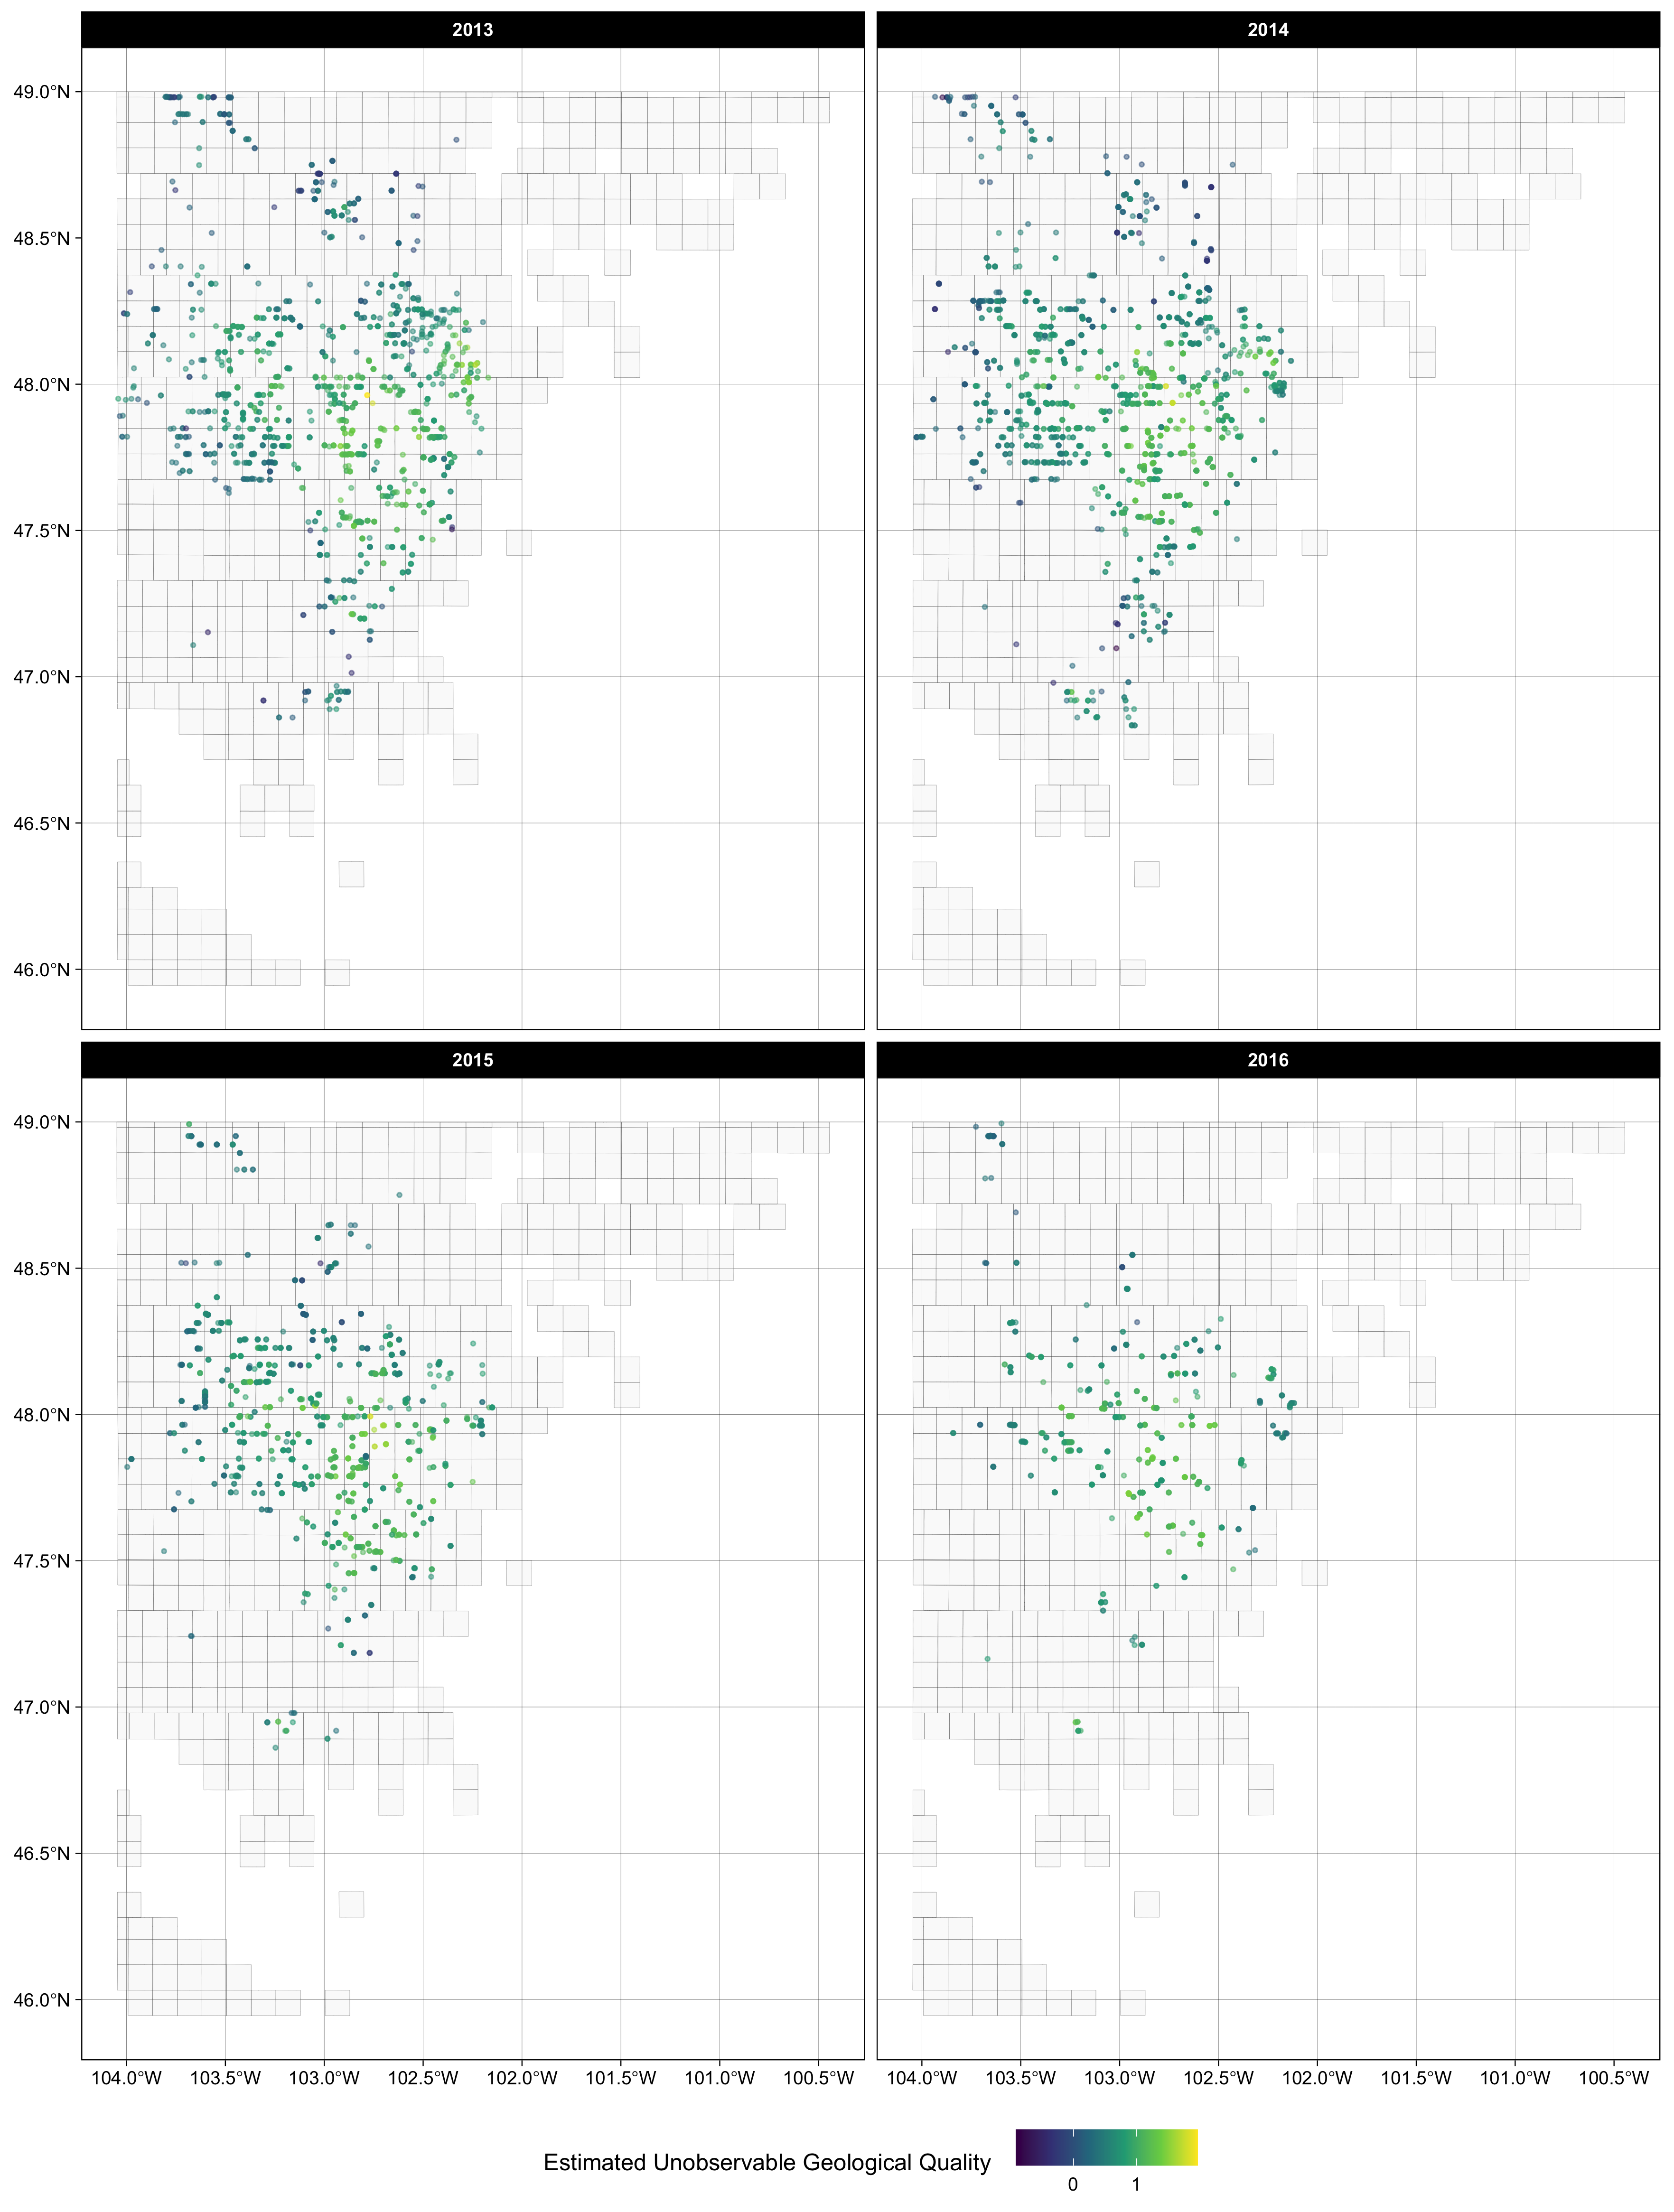
\includegraphics[scale = 0.105]{04_Chapter-3/00A_Figures/Figure_Cross-Sectional-Approach_Estimates-from-Robinson-Estimator_Spatial-Distribution-of-Unobservable-Geological-Quality.png}
        \caption{Spatial Distribution of the Estimated Geological Characteristic by Year}
        \caption*{
        	{\small
            \textit{Note}: 
            This figure illustrates the estimated geologic feature for each horizontal well completed between 2013 and 2016 by year. In this figure, each square is a section in the Public Land Survey System, whereas each dot indicates an individual well's geological characteristic. It is apparent that the share of drilling of horizontal wells with (relatively) small estimates decreased significantly starting in 2014, corresponding to the beginning of the oil price crash.
        }}
        \label{Figure:Spatial-Distribution-of-the-Estimated-Geological-Characteristic-by-Year}
    \end{figure}
%}

\begin{landscape}
%\afterpage{
    \begin{figure}[t!]
        \centering
        \includegraphics[scale = 0.13]{04_Chapter-3/00A_Figures/Figure_Spatial-Distributions-of-Geological-Characteristics.png}
        \caption{Spatial Distributions of Geological Characteristics}
        \caption*{
        	{\small
            \textit{Note}: 
            This figure depicts the spatial distributions of three geological features---thickness, thermal maturity, and total organic contents, which are available from the NDGS' geological survey data--- for the horizontal wells in our sample. In this figure, each square is a section in the Public Land Survey System, whereas each dot indicates an individual well's geological characteristic.  
        }}
        \label{Figure:Spatial-Distributions-of-Geological-Characteristics}
    \end{figure}
% }
\end{landscape}




% ------- Bibliography -------
\bibliographystyle{05_Bibliography/aea}
\bibliography{05_Bibliography/Bibliography}


\end{document}
